%% Rezolvari Mecanica %%

\section*{1. MECANICĂ}
1.1. Considerăm cele două particule care au masele $m$ şi $M=2 m$. Atunci, avem:

$$
\begin{aligned}
& m v=-m v_{1}^{\prime}+M v_{2}^{\prime} \\
& \frac{m v^{2}}{2}=-\frac{m v_{1}^{\prime 2}}{2}+\frac{M v_{2}^{\prime 2}}{2}
\end{aligned}
$$

Din aceste relații se obține:

$$
v_{1}^{\prime}=\frac{M-m}{M+m} v \text { si } v_{2}^{\prime}=\frac{2 m}{M+m} v .
$$

Energiile cinetice ale celor două particule sunt:

$$
E_{c_{1}}=\frac{m}{2}\left(\frac{M-m}{M+m}\right)^{2} v^{2}=\frac{1}{18} m v^{2}
$$

şi

$$
E_{c_{2}}=\frac{M}{2}\left(\frac{2 m}{M+m}\right)^{2} v^{2}=\frac{4}{9} m v^{2}
$$

1.2. $12960 \mathrm{~km} / \mathrm{h}^{2}=12960 \frac{1000}{3600^{2}}=1 \mathrm{~m} / \mathrm{s}^{2}$.\\
1.3. $\quad\left(m_{1}+m_{2}\right) v=m_{1} v_{1}$

$$
v=\frac{m_{1}}{\left(m_{1}+m_{2}\right)} v_{1}=\frac{200}{200+50} \cdot 5=4 \mathrm{~m} / \mathrm{s}
$$

1.4. $L=m(g+a) h=300(10+2) \cdot 5=18000 \mathrm{~J}=18 \mathrm{~kJ}$.\\
1.5. $\quad M v=m_{1} v_{1}+\left(M-m_{1}\right) v_{2} \Rightarrow$

$$
v_{2}=\frac{M v-m_{1} v_{1}}{M-m_{1}}=\frac{70 \cdot 320-30 \cdot 520}{70-30}=170 \mathrm{~m} / \mathrm{s}
$$

$$
\begin{aligned}
E_{c} & =\frac{m_{1} v_{1}^{2}}{2}+\frac{m_{2} v_{2}^{2}}{2}-\frac{M v^{2}}{2}=\frac{m_{1} v_{1}^{2}}{2}+\frac{1}{2}\left(M-m_{1}\right)\left(\frac{M v-m_{1} v_{1}}{M-m_{1}}\right)^{2}-\frac{M v^{2}}{2}= \\
& =\frac{1}{2} \frac{M \cdot m_{1}}{M-m_{1}}\left(v_{1}-v\right)^{2}=\frac{1}{2} \frac{70 \cdot 30}{70-30}(520-320)^{2}=1,05 \mathrm{MJ}
\end{aligned}
$$

1.6.

$$
\begin{aligned}
\Delta p & =m v \\
F_{m} & =\frac{\Delta p}{\Delta t}=\frac{2 m v}{\Delta t}=240 \mathrm{~N} .
\end{aligned}
$$

1.7. $\frac{s}{v}=\frac{d}{v_{1}+v_{2}}$

$$
s=\frac{d \cdot v}{v_{1}+v_{2}}=\frac{60 \cdot 88}{60+50}=48 \mathrm{~km}
$$

1.8. Răspuns corect: D)\\
1.9.

$$
\begin{aligned}
& m a=F_{2}-F_{1} \\
& a=\frac{F_{2}-F_{1}}{m}=\frac{7-3}{0,8}=5 \mathrm{~m} / \mathrm{s}^{2} .
\end{aligned}
$$

1.10.

$$
\left.\begin{array}{l}
\frac{m v_{\mathrm{P}}^{2}}{2}+E_{p_{\mathrm{P}}}=\frac{m v_{\mathrm{Q}}^{2}}{2}+E_{p_{\mathrm{Q}}} \\
E_{p_{\mathrm{P}}}=E_{p_{\mathrm{Q}}}+m g R \\
v_{\mathrm{P}}=0
\end{array}\right\} v_{\mathrm{Q}}=\sqrt{2 g R}=\sqrt{2 \cdot 10 \cdot 5}=10 \mathrm{~m} / \mathrm{s}
$$

1.11.

$$
\begin{aligned}
& v=v_{0}-g t \\
& E_{c}=\frac{m v^{2}}{2}=\frac{m}{2}\left(v_{0}-g t\right)^{2}=\frac{60 \cdot 10^{-3}}{2}(40-10 \cdot 1)^{2}=27 \mathrm{~J}
\end{aligned}
$$

1.12. $L=F_{m} \cdot d=\frac{F(x)+F\left(x_{0}\right)}{2}\left(x-x_{0}\right)=1,08 \mathrm{~kJ}$.\\
1.13. $\frac{m v^{2}}{2}=F x$

$$
F=\frac{m v^{2}}{2 x}=\frac{25 \cdot 10^{3} \cdot 0,3^{2}}{2 \cdot 3 \cdot 10^{-2}}=37,5 \mathrm{kN} .
$$

1.14. Răspuns corect: C)\\
1.15.

$$
m_{1} v_{1}+m_{2} v_{2}=\left(m_{1}+m_{2}\right) \cdot v
$$

$$
\begin{aligned}
Q & =E_{c}=m_{1} \frac{v_{1}^{2}}{2}+m_{2} \frac{v_{2}^{2}}{2}-\frac{1}{2}\left(m_{1}+m_{2}\right) \cdot v^{2}= \\
& =\frac{1}{2} \cdot \frac{m_{1} m_{2}}{m_{1}+m_{2}}\left(v_{1}-v_{2}\right)^{2}=\frac{1}{2} \cdot \frac{3 \cdot 2}{3+2}(2+3)^{2}=15 \mathrm{~J}
\end{aligned}
$$

1.16. Mişcarea este uniform accelerată ( $F=$ const.):

$$
\begin{aligned}
& v=a t \Rightarrow a=\frac{v}{t}=\frac{108000}{3600 \cdot 10}=3 \mathrm{~m} / \mathrm{s}^{2} \\
& S=\frac{a t^{2}}{2}=\frac{3 \cdot 100}{2}=150 \mathrm{~m}
\end{aligned}
$$

1.17. Componenta orizontală a forței resortului trebuie sǎ fie cel puțin egală cu forța de frecare (Fig. prob. 17):


\begin{align*}
& F_{0}=\mu\left(m g-F_{v}\right)  \tag{1}\\
& F_{0}=F \cos \alpha ; \quad F_{v}=F \sin \alpha ; \quad F=k \Delta x \tag{2}
\end{align*}


Ecuația (1) devine

$$
\begin{gathered}
k \Delta x \cos \alpha=\mu(m g-k \Delta x \sin \alpha) \\
\Delta x=\frac{\mu m g}{k(\cos \alpha+\mu \sin \alpha)} \\
E_{p}=\frac{k \Delta x^{2}}{2}=8,59 \mathrm{~J} .
\end{gathered}
$$

\begin{center}
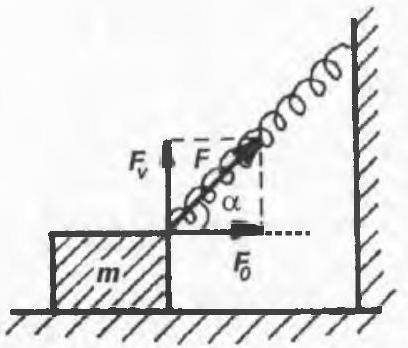
\includegraphics[max width=\textwidth]{2025_07_01_5b3ff9fa0d508c8e9f17g-201}
\end{center}

Fig. prob. 1.17\\
1.18. Conform conservării energiei:


\begin{equation*}
\frac{m v^{2}}{2}+m g h=\frac{m v_{0}^{2}}{2} \tag{1}
\end{equation*}


Dar $\frac{m v^{2}}{2}=\frac{1}{4} m g h$, ecuaţia (1) devine:

$$
\frac{1}{4} m g h+m g h=\frac{m v_{0}^{2}}{2} \Rightarrow h=\frac{2 v_{0}^{2}}{5 g}
$$

1.19. $L=m g h=G h=8400 \cdot 35=294000 \mathrm{~J}=294 \mathrm{~kJ}$.\\
1.20. $T_{1}=m_{1}(a+g) ; T_{2}=m_{2}(g-a)$

$$
\begin{gathered}
T_{1}=T_{2} \Rightarrow m_{1}(g+a)=m_{2}(g-a) \Rightarrow g\left(m_{2}-m_{1}\right)=a\left(m_{1}+m_{2}\right) \\
a=\frac{g\left(m_{2}-m_{1}\right)}{m_{1}+m_{2}}=\frac{10 \cdot 2}{10}=2 \mathrm{~m} / \mathrm{s}^{2} .
\end{gathered}
$$

1.21. $F=m_{1} a_{1}, \quad F=m_{2} a_{2}$

$$
F=\left(m_{1}+m_{2}\right) a \text { sau } F=\left(\frac{F}{a_{1}}+\frac{F}{a_{2}}\right) a
$$

Rezultǎ: $\quad a=\frac{a_{1} a_{2}}{a_{1}+a_{2}}=\frac{192}{32}=6 \mathrm{~m} / \mathrm{s}^{2}$.\\
1.22. $F=\sqrt{F_{1}^{2}+F_{2}^{2}}=5 \mathrm{~N}$

$$
m a=F-\mu m g=5-0,25 \cdot 20=0 ; \quad a=0 .
$$

\begin{center}
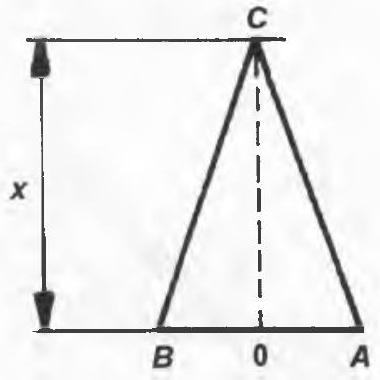
\includegraphics[max width=\textwidth]{2025_07_01_5b3ff9fa0d508c8e9f17g-202}
\end{center}

Fig. prob. 1.23\\
1.23. $A B=v t=26 \cdot 2=52 \mathrm{~m}$

$$
A C=v_{s} \frac{t}{2}=340 \frac{2}{2}=340 \mathrm{~m} .
$$

Conform Fig. prob. 1.23:

$$
x=\sqrt{A C^{2}-A O^{2}}=\sqrt{115600-676}=339 \mathrm{~m} .
$$

1.24. $a=g \sin \alpha$

$$
a \approx g \alpha=10 \cdot \frac{9}{\pi} \cdot \frac{\pi}{180}=\frac{1}{2} \mathrm{~m} / \mathrm{s}^{2}
$$

$$
\begin{aligned}
& v=v_{0}-a t \\
& \quad t=\frac{v_{0}-v}{a}=\frac{20-5}{\frac{1}{2}}=30 \mathrm{~s} .
\end{aligned}
$$

1.25. $h_{m}=\frac{g t_{c}^{2}}{2} \quad t_{c}=t_{u}=\frac{t}{2} ; h_{m}=\frac{g}{2} \frac{t^{2}}{4}=\frac{10 \cdot 16}{8}=20 \mathrm{~m}$.\\
1.26. Spațiul $\Delta S$ parcurs într-un interval $\Delta t=t_{2}-t_{1}$ este

$$
\begin{aligned}
\Delta S & =v_{0} t_{2}-\frac{a}{2} t_{2}^{2}-\left[v_{0} t_{1}-\frac{a}{2} t_{1}^{2}\right]= \\
& =v_{0}\left(t_{2}-t_{1}\right)-\frac{a}{2}\left(t_{2}^{2}-t_{1}^{2}\right)=\left(t_{2}-t_{1}\right)\left[v_{0}-\frac{a}{2}\left(t_{2}+t_{1}\right)\right]
\end{aligned}
$$

Aici $a=\mu g$. În cazul de față $t_{2}=5, t_{1}=4 \mathrm{deci}$

$$
5=20-\frac{\mu \cdot 10}{2} \cdot 9 \Rightarrow \mu=\frac{1}{3}
$$

1.27. Teorema conservării impulsului: $m_{1} v_{1}+m_{2} v_{2}=\left(m_{1}+m_{2}\right) \cdot v$

$$
v=\frac{m_{1} v_{1}+m_{2} v_{2}}{\left(m_{1}+m_{2}\right)}=\frac{21 \cdot 10^{3} \cdot 6+49 \cdot 10^{3} \cdot 3}{(21+49) 10^{3}}=3,9 \mathrm{~m} / \mathrm{s}
$$

1.28. Condiția pentru efectuarea buclei este ca în punctul cel mai de sus al buclei, forţa centrifugă să fie cel puțin egală cu greutatea

$$
\frac{m v^{2}}{r} \geq m g \Rightarrow r_{\max }=\frac{v^{2}}{g}=\frac{10^{4}}{10}=10^{3} \mathrm{~m}
$$

1.29. Forța centrifugă trebuie să fie cel mult egală cu greutatea:

$$
\frac{m v^{2}}{r} \leq m g \Rightarrow v_{\max }=\sqrt{r g}=15 \mathrm{~m} / \mathrm{s}
$$

1.30. Conservarea impulsului $m_{1} v_{1}-m_{2} v_{1}=m_{2} v$. Conservarea energiei cinetice $\frac{m_{1} v_{1}^{2}}{2}+\frac{m_{2} v_{1}^{2}}{2}=\frac{m_{2} v^{2}}{2}$. Din prima ecuație $v_{1}=\frac{m_{2} v}{m_{1}-m_{2}}$. Din cea de-a doua ecuație $v_{1}=\sqrt{\frac{m_{2} v^{2}}{m_{1}+m_{2}}}$. Egalându-le rezultă $\frac{m_{2}}{m_{1}}=3$.\\
1.31. În punctul cel mai de sus al traiectoriei $F_{1}=F_{c}-G=G$.

Conform legii lui Hooke $\Delta l_{1}=\frac{m g}{S E} l_{0}=\frac{10}{0,5 \cdot 10^{-6} \cdot 10^{11}}=2 \cdot 10^{-4} \mathrm{~m}$.

$$
l_{\min }=l_{0}+\Delta l_{1}=100,02 \mathrm{~cm}
$$

În punctul cel mai de jos al traiectoriei $F_{2}=F_{c}+G=3 G \Rightarrow$

$$
\begin{gathered}
\Delta l_{2}=\frac{3 m g}{S E} l_{0}=3 \Delta l_{1}=0,06 \mathrm{~cm} \\
l_{\max }=l_{0}+\Delta l_{2}=100,06 \mathrm{~cm}
\end{gathered}
$$

1.32. Pentru corpul $m_{1}$ :

$$
F-T-\mu m_{1} g=m_{1} a
$$

Pentru corpul $m_{2}$ :

$$
T-\mu m_{2} g=m_{2} a
$$

\begin{center}
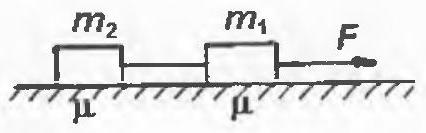
\includegraphics[max width=\textwidth]{2025_07_01_5b3ff9fa0d508c8e9f17g-203}
\end{center}

Fig. prob. 1.32

Multiplicând prima ecuaţie cu $m_{2}$ şi a doua cu $m_{1}$ rezultă $T=\frac{F m_{2}}{m_{1}+m_{2}}$\\
1.33. Acceleraţia de urcare $a_{u}=g(\sin \alpha+\mu \cos \alpha)$. Accelerația de coborâre $a_{c}=g(\sin \alpha-\mu \cos \alpha)$. Spațiul parcurs la urcare este acelaşi ca la coborâre:

$$
v_{0} t_{u}-\frac{a_{u} t_{u}^{2}}{2}=\frac{a_{c} t_{c}^{2}}{2}
$$

În punctul cel mai înalt $v=0$ deci $v_{0}=a_{u} t_{u}$.

Ecuaţia anterioară devine: $\frac{a_{u} t_{u}^{2}}{2}=\frac{a_{c} t_{c}^{2}}{2}$ Înlocuind $t_{u}=4 t_{c}$ rezultă $15 \sin \alpha=17 \mu \cos \alpha$ sau $\mu=\frac{15}{17} \operatorname{tg} \alpha=\frac{15}{17} \frac{\sqrt{3}}{3}=5 \frac{\sqrt{3}}{17}$.\\
1.34. Forma generală a ecuației unei mişcări uniform variate este $x=x_{0}+v_{0} t+\frac{a t^{2}}{2}$, deci rezultă $x_{0}=8 \mathrm{~m}, v_{0}=20 \mathrm{~m} / \mathrm{s} ; a=-4 \mathrm{~m} / \mathrm{s}^{2}$. Viteza în mişcarea uniform variată:

$$
v=v_{0}+a t=20-4 \cdot 2,3=10,8 \mathrm{~m} / \mathrm{s} .
$$

1.35. Ecuația vitezei în mişcarea uniform variată $v=v_{0}+a t$ deci $v_{0}=12 \mathrm{~m} / \mathrm{s}$; $a=-1 \mathrm{~m} / \mathrm{s}^{2}$. Ecuația coordonatei în mişcarea uniform variată:

$$
x=x_{0}+v_{0} t+\frac{a t^{2}}{2}=10+12 \cdot 8-\frac{1}{2} 64=74 \mathrm{~m} .
$$

1.36. $L=F_{f} l=\mu m g \cos \alpha l=m g l \sin \alpha=m g h=4,2 \cdot 10 \cdot 2,5=105 \mathrm{~J}$.\\
1.37. Viteza la un moment dat este rezultanta dintre viteza pe orizontală $v_{0}$ şi viteza pe verticală $v_{v}=g t$, adică $v=\sqrt{v_{0}^{2}+(g t)^{2}}$.

Creşterea este continuă, iar graficul nu este o dreaptă; deci comportarea este cea arătată de graficul C ).\\
1.38. Mişcarea este uniform variată fără viteză inițială. Conform ecuației lui Galilei

$$
v=\sqrt{2 a S}=\sqrt{2 \frac{F}{m}} l=\sqrt{2 \frac{p \cdot A}{m} l}=\sqrt{2 \frac{2 \cdot 10^{8} \cdot 80 \cdot 10^{-6}}{50 \cdot 10^{-3}} 0,25}=400 \mathrm{~m} / \mathrm{s} .
$$

1.39. $F=m a \Rightarrow a=\frac{F}{m}$

$$
\begin{aligned}
& a_{1}=\frac{F_{1}}{m}=\frac{9}{3}=3 \mathrm{~m} / \mathrm{s}^{2} ; a_{2}=\frac{F_{2}}{m}=\frac{4,5}{3}=1,5 \mathrm{~m} / \mathrm{s}^{2} \\
& v_{3}=a_{1} t_{1}=3 \cdot 3=9 \mathrm{~m} / \mathrm{s}
\end{aligned}
$$

În următoarele 2 s mişcarea este uniform accelerată cu $v_{3}$ ca viteză inițială şi accelerația $a_{2}$ :

$$
v_{5}=v_{3}+a_{2} t_{2}=9+1,5 \cdot 2=12 \mathrm{~m} / \mathrm{s}
$$

1.40. $G_{1}$ este egală cu tensiunea din fir. Descompunând $G$ după directia celor două fire:

$$
\frac{G}{2}=T \sin \alpha \text { deci } G_{1}=\frac{G}{2 \sin \alpha}
$$

Când $\alpha$ creşte, $\sin \alpha$ creşte, deci $G_{1}$ scade, dar nu sub formă de linie dreaptă, iar când $\alpha \rightarrow 0, G_{1}$ devine infinit; dependența este cea arătată de graficul C ).\\
1.41. Accelerația de frânare se obține din ecuația Galilei:

$$
v_{0}^{2}=2 a S \Rightarrow a=\frac{v_{0}^{2}}{2 S}=\frac{100}{2 \cdot 10}=5 \mathrm{~m} / \mathrm{s}^{2}
$$

Viteza de ciocnire se obține tot din ecuația Galilei:

$$
v=\sqrt{v_{0}^{2}-2 a d}=\sqrt{100-2 \cdot 5 \cdot 6,4}=6 \mathrm{~m} / \mathrm{s} .
$$

Impulsul $H=m v=800 \cdot 6=4800 \mathrm{kgm} / \mathrm{s}$.\\
1.42. Considerând sensul pozitiv al axei verticale în sus, viteza inițială este pozitivă. În timpul urcării viteza variază conform ecuației $v=v_{0}-g t$.

Când corpul ajunge la înălţimea maximă viteza este nulă. În timpul căderii $v=-g t$ deci este negativă şi creşte liniar în valoare absolută până ciocneşte placa. În acest moment își schimbă instantaneu sensul fără a-şi modifica mǎrimea. Ciclul se repetă nelimitat; deci comportarea este cea reprezentată de graficul B).\\
1.43. Considerăm momentul inițial $t=0$, momentul în care începe să cadă primul corp. Scriem legea vitezei pentru fiecare corp:

$$
\left\{\begin{array}{l}
v_{1}=g t_{1} \\
v_{2}=g t_{2}
\end{array}\right.
$$

unde $t_{2}=t_{1}-\tau$, obținem:

$$
\begin{aligned}
& v_{1}=g t_{1} \\
& v_{2}=g\left(t_{1}-\tau\right)=g t_{1}-g \tau=v_{1}-g \tau
\end{aligned}
$$

viteza relativă a primului corp față de al doilea este:

$$
v_{r}=v_{1}-v_{2}=v_{1}-\left(v_{1}-g \tau\right)=g \tau=\text { const. }
$$

Deci primul corp se mişcă cu viteza relativă constantă, față de al doilea.\\
Mişcarea lui este deci uniformă, în raport cu al doilea corp.\\
1.44. Scriind legea spațiului pentru cele două mobile (Fig. prob. 1.44):

$$
\begin{aligned}
& x=v_{1} t \\
& d+x=v_{2} t-\frac{a t^{2}}{2}
\end{aligned}
$$

Rezultă ecuația $a t^{2}-2\left(v_{2}-v_{1}\right) t+2 d=0$.

Soluțiile ecuației sunt: $t_{1,2}=\frac{\left(v_{2}-v_{1}\right) \pm \sqrt{\left(v_{2}-v_{1}\right)^{2}-2 a d}}{d}$.\\
Pentru a se întâlni o singură dată, trebuie ca rădǎcinile ecuației să fie confundate: $t_{1}=t_{2} \Rightarrow d=\frac{\left(v_{2}-v_{1}\right)^{2}}{2 a}$, timpul până la întâlnire este:

$$
t=\frac{v_{2}-v_{1}}{a}=\frac{5}{0,1}=50 \mathrm{~s} .
$$

Spațiul parcurs de primul mobil până la întâlnire este $x=v_{1} t=5 \cdot 50=250 \mathrm{~m}$.\\
(1)\\
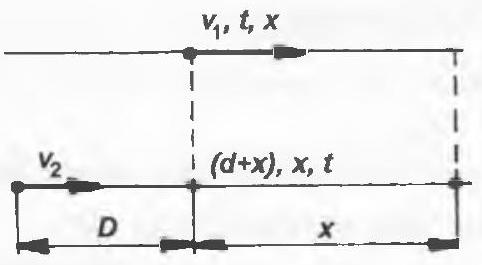
\includegraphics[max width=\textwidth, center]{2025_07_01_5b3ff9fa0d508c8e9f17g-206(1)}\\
(2)

Fig. prob. 1.44\\
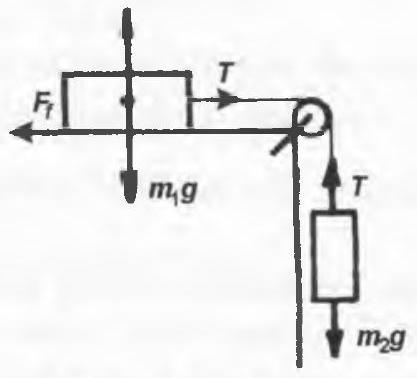
\includegraphics[max width=\textwidth, center]{2025_07_01_5b3ff9fa0d508c8e9f17g-206}

Fig. prob. 1.45\\
1.45. Scriem legea a 2-a a dinamicii pentru fiecare corp (Fig. prob. 1.45):

$$
\begin{aligned}
& T-\mu m_{1} g=m_{1} a_{1} \\
& m_{2} g-T=m_{2} a_{1}
\end{aligned}
$$

Rezolvând sistemul obținem $a_{1}=\frac{m_{2}-\mu m_{1}}{m_{1}+m_{2}} g$.\\
Inversând corpurile şi scriind din nou legea a doua a dinamicii obținem:

$$
a_{2}=\frac{m_{1}-\mu m_{2}}{m_{1}+m_{2}} g \Rightarrow \frac{a_{1}}{a_{2}}=\frac{m_{2}-\mu m_{1}}{m_{1}-\mu m_{2}}=\frac{3 m_{1}-0,15 m_{1}}{m_{1}-0,15 m_{1}}=5,18 .
$$

1.46. Vezi Fig. prob. 1.46.

$$
\begin{aligned}
& C A-C B=d \\
& C B=t_{1} v_{1} \\
& C A=t_{2} v_{2} \\
& t_{2} v_{2}-t_{1} v_{1}=d
\end{aligned}
$$

Primul biciclist parcurge distanta AC în timpul $t_{1}=\frac{A C}{v_{1}}=\frac{v_{2} t_{2}}{v_{1}}$.\\
Al doilea parcurge distanta BC în timpul $t_{2}=\frac{v_{1} t_{1}}{v_{2}}$.

Deoarece $t_{1}=t_{2}$, avem $\frac{v_{1}}{v_{2}}=\frac{\sqrt{t_{2}}}{\sqrt{t_{1}}} \Rightarrow$

$$
\begin{aligned}
& v_{1}=\frac{d \sqrt{t_{2}}}{t_{2} \sqrt{t_{1}}-t_{1} \sqrt{t_{2}}}=2 \mathrm{~m} / \mathrm{s} \\
& v_{2}=\frac{d \sqrt{t_{1}}}{t_{2} \sqrt{t_{1}}-t_{1} \sqrt{t_{2}}}=1,42 \mathrm{~m} / \mathrm{s}
\end{aligned}
$$

1.47. Din Fig. prob. 1.47 a:\\
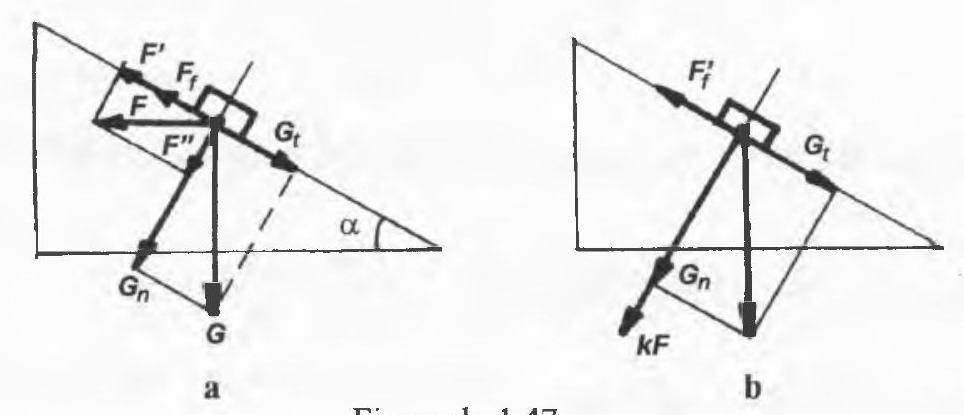
\includegraphics[max width=\textwidth, center]{2025_07_01_5b3ff9fa0d508c8e9f17g-207}

Fig. prob. 1.47

$$
\begin{aligned}
& F^{\prime}+F_{f}=G_{t} \\
& G_{t}=m g \sin \alpha \\
& F^{\prime}=F \cos \alpha \\
& F_{f}=\mu\left(G_{n}+F^{n}\right)=\mu(m g \cos \alpha+F \sin \alpha)
\end{aligned}
$$

Din Fig. prob. $1.47 \mathrm{~b}: G_{t}=F_{f}^{\prime}$.

$$
\begin{aligned}
& F_{f}=\mu\left(G_{n}+k F\right) \\
& F_{f}^{\prime}=\mu(m g \cos \alpha+k F)
\end{aligned} \Rightarrow \quad k \mu=\cos \alpha+\mu \sin \alpha \Rightarrow \mu=\frac{\cos \alpha}{k-\sin \alpha}
$$

1.48. Dacă $v_{0}$ este viteza inițială a corpului:

$$
\begin{aligned}
a_{u} & =g(\sin \alpha+\mu \cos \alpha) \\
a_{c} & =g(\sin \alpha-\mu \cos \alpha) \\
t_{u} & =\frac{v_{0}}{a_{u}} ; s_{o p}=\frac{v_{0}^{2}}{2 a_{u}} \\
t_{c} & =\sqrt{\frac{2 s_{o p}}{a_{c}}}=\sqrt{\frac{v_{0}^{2}}{g^{2}\left(\sin ^{2} \alpha-\mu^{2} \cos ^{2} \alpha\right)}}
\end{aligned}
$$

\begin{center}
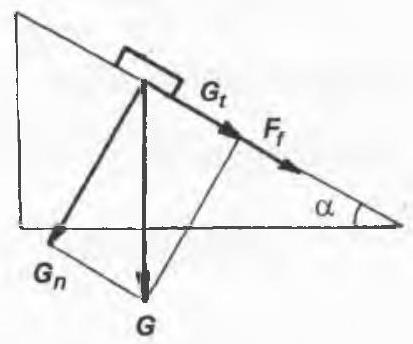
\includegraphics[max width=\textwidth]{2025_07_01_5b3ff9fa0d508c8e9f17g-207(1)}
\end{center}

Fig. 1.48

Condiția impusă în enunţ este $t_{c}=k t_{u}: \quad k^{2} \sin \alpha-k^{2} \mu \cos \alpha=\sin \alpha+\mu \cos \alpha$

$$
\mu=\frac{k^{2}-1}{k^{2}+1} \operatorname{tg} \alpha=0,055 .
$$

1.49. Din enunt: $E_{c}=E_{p}$,

$$
\begin{gathered}
\frac{m v^{2}}{2}=m g h \quad \frac{m v^{2}}{2}=m g\left(v_{0} t-g \frac{t^{2}}{2}\right) \\
\left(v_{0} t-g t\right)^{2}=2 g v_{0} t-g^{2} t^{2} \quad 2 g^{2} t^{2}-4 v_{0} g t+v_{0}^{2}=0 \\
t_{1,2}=\frac{v_{0}(2 \pm \sqrt{2})}{2 g} .
\end{gathered}
$$

1.50. a) Dacă notǎm cu $T_{0}$, perioada orarului și cu $T_{m}$, perioada numitorului avem:

$$
\begin{aligned}
& \alpha_{m}-\alpha_{0}=\frac{\pi}{2}, \quad\left(\omega_{m}-\omega_{0}\right) t=\frac{\pi}{2}, \quad\left(\frac{2 \pi}{T_{m}}-\frac{2 \pi}{T_{0}}\right) t=\frac{\pi}{2} \\
& \Rightarrow t=\frac{T_{0} \cdot T_{m}}{4\left(T_{0}-T_{m}\right)}=16,36 \mathrm{~min} .
\end{aligned}
$$

b) $\alpha_{m}-\alpha_{0}=2 \pi$

$$
\Rightarrow t=\frac{T_{0} \cdot T_{m}}{T_{0}-T_{m}}=65,45 \mathrm{~min}=1,09 \mathrm{~h}
$$

unde

$$
\begin{aligned}
& T_{0}=12 \mathrm{~h}=12 \cdot 3600=43.200 \mathrm{~s} \\
& T_{m}=1 \mathrm{~h}=3600 \mathrm{~s}
\end{aligned}
$$

1.51. Se cere: $h_{\max }=\frac{v_{0}^{2}}{2 g}$.

Pentru primul corp: $\quad h=\frac{g t_{1}^{2}}{2} \Rightarrow t_{1}=\sqrt{2 h / g}$\\
Pentru al doilea corp: $\quad t_{2}=t_{u_{2}}+t_{c_{2}}=2 t_{u_{2}}=2 \frac{v_{0}}{g}$.\\
Din condiția ca $t_{1}=t_{2}$ rezultă:

$$
\sqrt{2 h / g}=2 \frac{v_{0}}{g} \Rightarrow \frac{2 h}{g}=4 \frac{v_{0}^{2}}{g^{2}} \Rightarrow v_{0}^{2}=\frac{h g}{2} \Rightarrow h_{\max }=\frac{h}{4} .
$$

1.52. Se cunoaşte: $h_{\text {max }_{1}}=\frac{v_{01}^{2}}{2 g}$, unde $v_{01}$ este viteza inițială după ciocnire.

Pe de altă parte, energia la coborâre este egală cu energia la pornire și deoarece se pierde jumătate rezultă:

$$
\frac{1}{2}\left(\frac{m v_{0}^{2}}{2}\right)=\frac{1}{2}\left(\frac{m v_{01}^{2}}{2}\right) \Rightarrow v_{01}=\frac{v_{0}}{\sqrt{2}}=\frac{v_{0} \sqrt{2}}{2} .
$$

Prin urmare:

$$
h_{\max _{1}}=\frac{v_{01}^{2}}{2 g}=\frac{1600}{40}=40 \mathrm{~m}
$$

1.53. Pentru primul corp:

$$
h_{0}=\frac{g t_{1}^{2}}{2} \Rightarrow t_{1}=\sqrt{2 h_{0} / g}=\sqrt{\frac{490}{10}}=7 \mathrm{~s}
$$

Pentru al doilea corp:

$$
h_{0}^{\prime}=\frac{g\left(t_{1}-2\right)^{2}}{2}=\frac{10 \cdot 5^{2}}{2}=125 \mathrm{~m}
$$

Rezultă:

$$
\Delta h=h_{0}-h_{0}^{\prime}=245-125=120 \mathrm{~m} .
$$

1.54. Datorită legii conservării energiei:

$$
\begin{gathered}
m g l\left(1-\cos \alpha_{i}\right)=\frac{m v_{i}^{2}}{2} \Rightarrow v_{i}=\sqrt{2 g l\left(1-\cos \alpha_{i}\right)} \\
\Rightarrow \frac{v_{1}}{v_{2}}=\sqrt{\frac{1-\cos \alpha_{1}}{1-\cos \alpha_{2}}} \cong 1,478
\end{gathered}
$$

1.55. Conform teoremei variației energiei cinetice, pentru prima scândură se poate scrie:

$$
0-\frac{m v_{0}^{2}}{2}=F_{r} d \cos 180^{\circ} \Rightarrow F_{r}=\frac{m v_{0}^{2}}{2 d}
$$

Pentru a doua scândură:

$$
\begin{aligned}
& \frac{m v^{2}}{2}-\frac{m v_{0}^{2}}{2}=F_{r} \frac{d}{2} \cos 180^{\circ} \Rightarrow \frac{m v^{2}}{2}=\frac{m v_{0}^{2}}{4} \Rightarrow \\
& v=v_{0} / \sqrt{2}=v_{0} \sqrt{2} / 2=\frac{1,41}{2} \cdot 200=141 \mathrm{~m} / \mathrm{s}
\end{aligned}
$$

1.56. $P=L / t=\frac{F_{t r} \cdot S}{t}=F_{t r} \cdot v$

În primul caz, $F_{t r}=m a+\mu m g \Rightarrow$

$$
a=\frac{P}{m v}-\mu g=\frac{400 \cdot 10^{3}}{200 \cdot 10^{3} \cdot 2}-0,01 \cdot 10=0,9 \mathrm{~m} / \mathrm{s}^{2}
$$

În cazul al doilea, $F_{t r}=F_{f r}=\mu m g$

$$
P=\mu m g v_{\max } \Rightarrow v_{\max }=\frac{P}{\mu m g}=\frac{400 \cdot 10^{3}}{0,01 \cdot 200 \cdot 10^{3} \cdot 10}=20 \mathrm{~m} / \mathrm{s} .
$$

\begin{center}
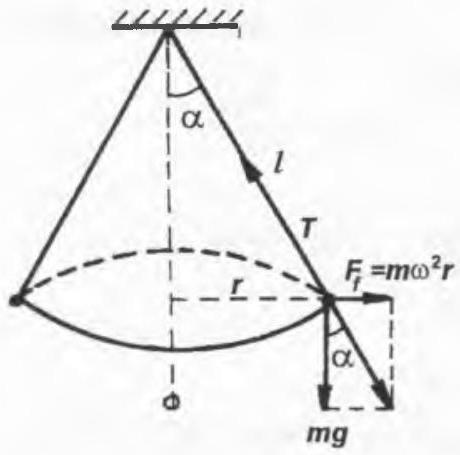
\includegraphics[max width=\textwidth]{2025_07_01_5b3ff9fa0d508c8e9f17g-210}
\end{center}

Fig. prob. 1.57\\
1.57. Vezi Fig. prob. 1.57.

$$
\begin{aligned}
\operatorname{tg} \alpha=\frac{m \omega^{2} r}{m g} & =\frac{\omega^{2} r}{g} \\
& \frac{\sin \alpha}{\cos \alpha}=\frac{\omega^{2}}{g} l \sin \alpha \\
\omega & =\sqrt{g / l \cos \alpha} \Rightarrow \\
T & =\frac{2 \pi}{\omega}=2 \pi \sqrt{\frac{l \cos \alpha}{g}}
\end{aligned}
$$

1.58. $s_{1}=\frac{a t_{1}^{2}}{2} \Rightarrow a=\frac{2 s_{1}}{t_{1}^{2}}=\frac{2 \cdot 0,5}{1}=1 \mathrm{~m} / \mathrm{s}^{2} ; t_{1}=1 \mathrm{~s} ; v_{2}=a t_{2}=1 \cdot 2=2 \mathrm{~m} / \mathrm{s}$; $t_{2}=2 \mathrm{~s} ; E_{c}=\frac{m v_{2}^{2}}{2}=\frac{1 \cdot 2^{2}}{2}=2 \mathrm{~J}$.\\
1.59. $s_{1}=v_{0} t_{1}+\frac{a t_{1}^{2}}{2} \Rightarrow v_{0}=\frac{s_{1}-\frac{a t_{1}^{2}}{2}}{t_{1}} ; s_{2}=v_{0} t_{2}+\frac{a t_{2}^{2}}{2}=\left(v_{0}+a t_{1}\right) t_{2}+\frac{a t_{2}^{2}}{2}$ $s_{2}=\left(\frac{s_{1}-a t_{1}^{2} / 2}{t_{1}}+a t_{1}\right) t_{2}+\frac{a t_{2}^{2}}{2} ; \quad s_{2} t_{1}=s_{1} t_{2}-\frac{a t_{1}^{2} t_{2}}{2}+a t_{1}^{2} t_{2}+\frac{a t_{2}^{2} t_{1}}{2} ;$\\
$a=\frac{2\left(s_{2} t_{1}-s_{1} t_{2}\right)}{t_{1} t_{2}\left(t_{1}+t_{2}\right)}=\frac{2 \cdot 1 \cdot(2-1)}{1 \cdot 1(2)}=1 \mathrm{~m} / \mathrm{s}^{2} ; t_{1}=1 \mathrm{~s}: \mathrm{s}_{1}=1 \mathrm{~m} ; \quad t_{2}=1 \mathrm{~s}: \mathrm{s}_{2}=2 \mathrm{~m}$.\\
1.60. $a=g \frac{m_{2}-m_{1}}{m_{1}+m_{2}}=10 \cdot \frac{0,1}{0,5}=2 \mathrm{~m} / \mathrm{s}^{2} ; t=\sqrt{\frac{s}{a}}=\sqrt{\frac{2}{2}}=1 \mathrm{~s}$.\\
1.61. $h=h_{1}+h_{2}=v_{01} t-\frac{g t^{2}}{2}+v_{02} t+\frac{g t^{2}}{2}=\left(v_{01}+v_{02}\right) t$;

$$
\begin{array}{ll}
t=\frac{h}{v_{01}+v_{02}}=\frac{100}{80+20}=1 \mathrm{~s} ; & v_{1}=v_{01}-g t=80-10=70 \mathrm{~m} / \mathrm{s} ; \\
v_{2}=v_{02}-g t=20+10=30 \mathrm{~m} / \mathrm{s} ; & m_{1} v_{1}-m_{2} v_{2}=\left(m_{1}+m_{2}\right) v ;
\end{array}
$$

$$
\begin{aligned}
& v=\frac{m_{1} v_{1}-m_{2} v_{2}}{m_{1}+m_{2}}=\frac{70 \cdot 1-30 \cdot 1}{2}=20 \mathrm{~m} / \mathrm{s} ; \\
& E_{c}=\frac{\left(m_{1}+m_{2}\right) v^{2}}{2}=\frac{2 \cdot 400}{2}=400 \mathrm{~J} .
\end{aligned}
$$

1.62. $L=P \cdot t=P \cdot \frac{v_{2}-v_{1}}{a}=P \cdot \frac{v_{2}-v_{1}}{v_{2}^{2}-v_{1}^{2}} \cdot 2 d=\frac{2 P d}{v_{2}+v_{1}}$;\\
$v_{2}^{2}=v_{1}^{2}+2 a d \Rightarrow a=\frac{v_{2}^{2}-v_{1}^{2}}{2 d} ; d=\frac{L\left(v_{2}+v_{1}\right)}{2 P}=\frac{3 \cdot 10^{5} \cdot 25}{2 \cdot 3 \cdot 10^{4}}=\frac{250}{2}=125 \mathrm{~m}$.\\
1.63. $F_{f}+G \sin \alpha=F \cos \alpha ; \quad \mu(G \cos \alpha+F \sin \alpha)=F \cos \alpha-G \sin \alpha ;$ (Fig. prob. 1.63).

$$
\mu=\frac{a \cos \alpha-g \sin \alpha}{g \cos \alpha+a \sin \alpha}=\frac{a-g \operatorname{tg} \alpha}{g+a \operatorname{tg} \alpha}=\frac{15-10}{10+15}=\frac{5}{25}=0,2 .
$$

\begin{center}
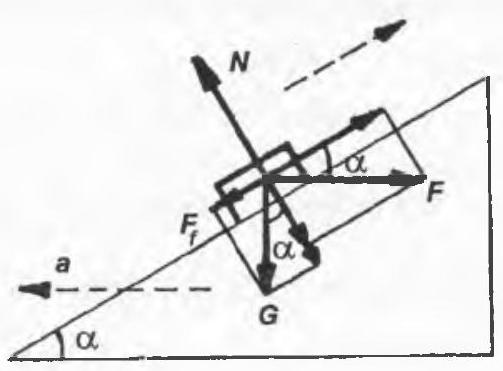
\includegraphics[max width=\textwidth]{2025_07_01_5b3ff9fa0d508c8e9f17g-211}
\end{center}

Fig. prob. 1.63\\
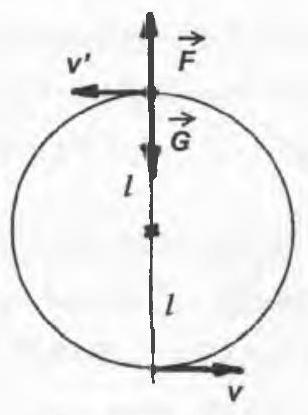
\includegraphics[max width=\textwidth, center]{2025_07_01_5b3ff9fa0d508c8e9f17g-211(1)}

Fig. prob. 1.65\\
1.64. $F_{t}=m a+F_{f}=m \frac{v}{t}+\mu m g ; \frac{m v}{t}=F_{t}-\mu m g \Rightarrow t=\frac{m v}{F_{t}-\mu m g}=$

$$
=\frac{10^{6} \cdot 20}{5 \cdot 10^{5}-0,05 \cdot 10 \cdot 10^{6}}=\frac{2 \cdot 10^{7}}{2 \cdot 10^{5}}=100 \mathrm{~s}
$$

1.65. Fig. prob. 1.65.

$$
\begin{aligned}
& m v_{0}=(M+m) v \Rightarrow v=\frac{m v_{0}}{M+m} ; \\
& \frac{(M+m) v^{2}}{2}=(M+m) g \cdot 2 l+\frac{(M+m) v^{\prime 2}}{2} ; v^{2}=4 g l+v^{\prime 2}=5 g l ; \\
& \frac{(M+m) v^{\prime 2}}{l}=(M+m) g ; \quad v^{\prime 2}=g l ;
\end{aligned}
$$

$$
\left(\frac{m}{M+m}\right)^{2} v_{0}^{2}=5 g l \Rightarrow v_{0}=\frac{M+m}{m} \sqrt{5 g l}=1000 \mathrm{~m} / \mathrm{s} .
$$

1.66. $F\left(x_{1}\right)=k x_{1} \Rightarrow k=\frac{F\left(x_{1}\right)}{x_{1}}=10 \frac{\mathrm{~N}}{\mathrm{~m}}$;

$$
L=\frac{F\left(x_{1}\right)+F\left(x_{2}\right)}{2}\left(x_{2}-x_{1}\right)==\frac{10+20}{2} \cdot 1=15 \mathrm{~J} .
$$

1.67. $T-m g=0 \Rightarrow T=m g$\\
$T_{1} \sin \alpha_{1}+T_{2} \sin \alpha_{2}-T=0 \Rightarrow T_{1}=\left(m g \cos \alpha_{2}\right) / \sin \left(\alpha_{1}+\alpha_{2}\right)$\\
$-T_{1} \cos \alpha_{1}+T_{2} \cos \alpha_{2}=0 \Rightarrow T_{2}=\left(m g \cos \alpha_{1}\right) / \sin \left(\alpha_{1}+\alpha_{2}\right)$\\
$T=2 \cdot 9,8 \mathrm{~N}=19,6 \mathrm{~N} ; \quad T_{1}=2 \cdot 9,8\left(\sin 30^{\circ}\right) \mathrm{N}=9,8 \mathrm{~N}$; $T_{2}=2 \cdot 9,8\left(\cos 30^{\circ}\right) \mathrm{N}=9,8 \sqrt{3} \mathrm{~N}$.\\
1.68. $\mu N+m_{1} g \sin \alpha-T=m_{1} a_{1} ; \quad N-\mu m_{1} g \cos \alpha=0$;\\
$m_{2} g-T=m_{2} a_{2} ; \quad x_{1}+x_{2}=$ const., $\quad a_{1}+a_{2}=0 \Rightarrow$\\
$\mu m_{1} g \cos \alpha+m_{1} g \sin \alpha-T=m_{1} a_{1} ; m_{2} g-T=m_{2} a_{2}$;

$$
x_{1}+x_{2}=\text { const. } ; \quad a_{1}+a_{2}=0
$$

1.69. $T-m_{1} g \sin \alpha_{1}=m_{1} a$;\\
$m_{2} g \sin \alpha_{2}-T=m_{2} a$;\\
$a=g\left(m_{2} \sin \alpha_{2}-m_{1} \sin \alpha_{1}\right) /\left(m_{1}+m_{2}\right)$;\\
$\sin \alpha_{1}=1 / 2, \sin \alpha_{2}=\sqrt{2} / 2$;

$$
a=(2 \cdot \sqrt{2} / 2-1 / 2) \cdot 9,8 / 3 \mathrm{~m} / \mathrm{s}^{2}=2,97 \mathrm{~m} / \mathrm{s}^{2} .
$$

1.70. $v_{1}=v_{0}-g t, \quad v_{2}=g(t-\Delta t) \Rightarrow$

$$
v_{r}=v_{2}-\left(-v_{1}\right)=v_{2}-v_{1}=v_{0}-g t+g t-g \Delta t=v_{0}-g \Delta t .
$$

1.71. $G_{t}=G \sin \alpha=m g \sin \alpha ; G_{n}=G \cos \alpha=m g \cos \alpha$;\\
$F_{r}=\mu G_{n}=\mu m g \cos \alpha ; G_{t}>F_{f} \Rightarrow m g \sin \alpha>\mu m g \cos \alpha \Rightarrow \operatorname{tg} \alpha>\mu$.\\
1.72. $x=2 \pi R / 4=\pi R / 2 \Rightarrow R=2 x / \pi=2 \cdot 314 / \pi=200 \mathrm{~m}$.\\
1.73. $L=F \cdot h=m(g+a) h=1 \cdot(9,8+0,19) \cdot 10=100 \mathrm{~J}$.\\
1.74. $a=0, F_{r}=m g \Rightarrow m=F_{r} / g=(98,1 / 9,81) \mathrm{kg}=10 \mathrm{~kg}$.\\
1.75. $v_{m}=x / t=x /\left(t_{1}+t_{2}\right)=x /\left(x /\left(2 v_{1}\right)+x /\left(2 v_{2}\right)\right)=1 /\left(1 /\left(2 v_{1}\right)+1 /\left(2 v_{2}\right)\right)=$ $=2 v_{1} v_{2} /\left(v_{1}+v_{2}\right)=2 \cdot 6 \cdot 4 /(6+4) \mathrm{km} / \mathrm{h}=4,8 \mathrm{~km} / \mathrm{h}$.\\
1.76. $F=\left(m_{1}+m_{2}\right) a \Rightarrow a=F /\left(m_{1}+m_{2}\right)=6 /(2+1) \mathrm{m} / \mathrm{s}^{2}=2 \mathrm{~m} / \mathrm{s}^{2}$.\\
1.77. $m_{2} v_{0}=\left(m_{1}+m_{2}\right) v \Rightarrow v=m_{2} v_{0} /\left(m_{1}+m_{2}\right)=2 \cdot 30 /(10+2)=5 \mathrm{~m} / \mathrm{s}$.\\
1.78. Se poate utiliza teorema variaţiei energiei cinetice (Fig. prob. 1.78):

$$
0-\frac{m v^{2}}{2}=-m g \sin \alpha l-\mu m g \cos \alpha l
$$

adicǎ $E=L_{1}+L_{2}(1)$, unde $L_{1}=m g \sin \alpha l$ este lucrul mecanic al greutațiii tangențiale, iar\\
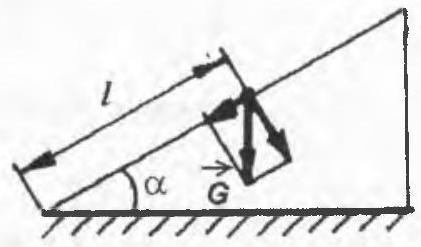
\includegraphics[max width=\textwidth, center]{2025_07_01_5b3ff9fa0d508c8e9f17g-213}

Fig. prob. 1.78 $L_{2}=\mu m g \cos \alpha l$ este lucrul mecanic al forței de frecare. Se vede că $\frac{L_{2}}{L_{1}}=\mu \operatorname{ctg} \alpha$ (2). Din (1) şi (2): $L_{2}=\frac{\mu E}{\mu+\operatorname{ctg} \alpha}=\frac{0,2 \cdot 24}{0,2+1}=4 \mathrm{~J}$.\\
1.79. Accelerația de cădere este $a=\frac{2 h}{t^{2}}$. Pe de altă parte: $m a=m g-R$, deci $R=m(g-a)=m\left(g-\frac{2 h}{t^{2}}\right)=1,88 \mathrm{~N}$.\\
1.80. Din legea conservării energiei, rezultă: $m g h+\frac{m v^{2}}{2}=m g h^{\prime}$, de unde $v=\sqrt{2 g\left(h^{\prime}-h\right)}=2 \mathrm{~m} / \mathrm{s}$.\\
1.81. Fig. prob. 1.81: $R=M g-m g \sin \alpha ; R=607,6 \mathrm{~N}$.\\
1.82. $P=\frac{L}{t}=\frac{m g h}{t}=\frac{75 \cdot 10 \cdot 18}{3 \cdot 60}=75 \mathrm{~W}$.\\
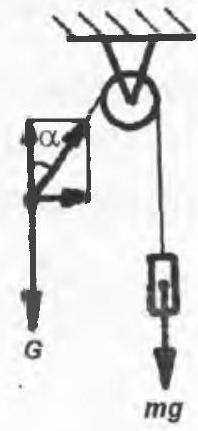
\includegraphics[max width=\textwidth, center]{2025_07_01_5b3ff9fa0d508c8e9f17g-213(2)}

Fig. prob. 1.81\\
1.83. Timpii de urcare $\left(t_{1}\right)$ şi de coborâre $\left(t_{2}\right)$ sunt egali, $t_{1}=2 \mathrm{~s} \Rightarrow$ $h=\frac{g t_{1}^{2}}{2}=20 \mathrm{~m}$.\\
1.84. Firul se orientează după rezultanta dintre forţa de greutate ( $m g$ ) şi forţa de inerție ( $m a$ ) (Fig. prob. 1.84): $\operatorname{tg} \alpha=\frac{m a}{m g}=\frac{a}{g}, a=g \operatorname{tg} \alpha=5,66 \mathrm{~m} / \mathrm{s}$.\\
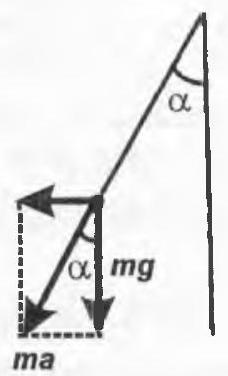
\includegraphics[max width=\textwidth, center]{2025_07_01_5b3ff9fa0d508c8e9f17g-213(1)}

Fig. prob. 1.84\\
1.85. Din legea impulsului: $m_{A} v=\left(m_{A}+m_{B}\right) v^{\prime}$ cu $v^{\prime}=\sqrt{2 a l}=\sqrt{2 \mu g l}$, rezultǎ $v=\frac{m_{A}+m_{B}}{m_{A}} \sqrt{2 \mu g l}=1 \mathrm{~m} / \mathrm{s}$.\\
1.86. Fie un sistem de coordonate ataşat sistemului ca în Fig. prob. 1.86. Coordonatele celor 2 mobile, A respectiv B la un moment $t$ vor fi:

$$
\begin{aligned}
& x_{A}=0 ; y_{A}=v t-\frac{g t^{2}}{2} \\
& x_{B}=v t \cos \alpha ; y_{B}=h+v t \sin \alpha-\frac{g t^{2}}{2}
\end{aligned}
$$

\begin{center}
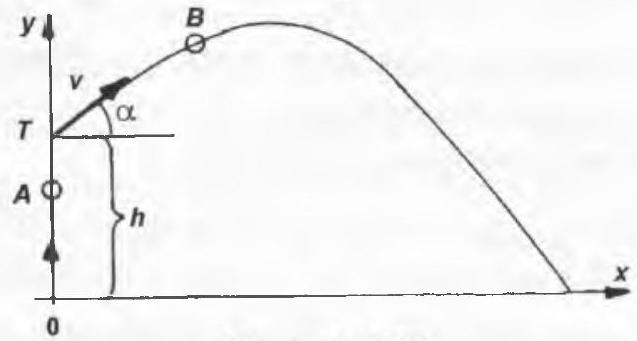
\includegraphics[max width=\textwidth]{2025_07_01_5b3ff9fa0d508c8e9f17g-214(1)}
\end{center}

Fig. prob. 1.86\\
Corespunzător, distanta dintre cele două mobile va fi:

$$
d=\sqrt{\left(x_{B}-x_{A}\right)^{2}+\left(y_{B}-y_{A}\right)^{2}}=\sqrt{(v t \cos \alpha)^{2}+[h+v t(\sin \alpha-1)]^{2}}
$$

Minimul distanţei este dat de ecuația $d^{\prime}(t)=0$; obținem timpul la care distanța este minimă şi această distanță:

$$
t=\frac{h}{2 \cdot v}=1 \mathrm{~s} ; d_{\text {minim }}=h \cdot \sqrt{\frac{1+\sin (\alpha)}{2}}=20 \cdot \sqrt{3} \mathrm{~m}
$$

1.87. Planul înclinat împreună cu corpul se\\
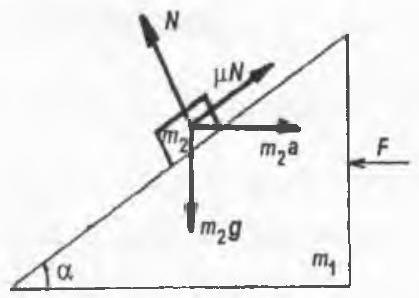
\includegraphics[max width=\textwidth, center]{2025_07_01_5b3ff9fa0d508c8e9f17g-214}

Fig. prob. 1.87. deplasează sub acțiunea forței $F$ (fig. prob. 1.87) cu acceleraţia $a=\frac{F}{m_{1}+m_{2}}=1,875 \mathrm{~m} / \mathrm{s}^{2}$. Observăm că\\
$m_{2} g \cos \alpha=0,1875 \mathrm{~N}<m_{2} g \sin \alpha=1,697 \mathrm{~N}$.\\
Astfel, corpul de masă $m_{2}$ coboară pe planul înclinat cu accelerația

$$
a^{\prime}=g(\sin \alpha-\mu \cos \alpha)-a(\cos \alpha+\mu \sin \alpha)=5,575 \mathrm{~m} / \mathrm{s}^{2}
$$

1.88. Fie $d_{1}, d_{2}$, şi $d_{3}$ alungirile absolute ale firului pendulului în poziția de elongație maximă $\alpha$, în poziția verticală unde viteza este maximă $v_{\text {max }}$, respectiv\\
în poziția căutată în problemă. În acest caz, principiul echilibrului forțelor respectiv cel al conservării energiei mecanice, oferă ecuațiile:

$$
\begin{aligned}
& k\left(L+d_{1}\right)=m g \cos \alpha \\
& k\left(L+d_{2}\right)=m g+\frac{m v_{\max }^{2}}{L+d_{2}} \\
& \frac{k d_{1}^{2}}{2}+m g\left(L+d_{2}-\left(L+d_{1}\right) \cos \alpha\right)=\frac{k d_{2}^{2}}{2}+\frac{m v_{\max }^{2}}{2} \\
& k\left(L+d_{3}\right)=m g \cos \beta+\frac{m\left(\frac{v_{\max }}{2}\right)^{2}}{L+d_{3}} \\
& \frac{k d_{1}^{2}}{2}+m g\left[L+d_{2}-\left(L+d_{1}\right) \cos \alpha\right]= \\
& =\frac{k d_{3}^{2}}{2}+\frac{m\left(\frac{v_{\max }}{2}\right)^{2}}{2}+m g\left[L+d_{2}-\left(L+d_{3}\right) \cos \beta\right]
\end{aligned}
$$

Rezolvând sistemul în necunoscutele $d_{1}, d_{2}, d_{3}, v_{\text {max }}$ şi $\cos \beta$, obținem răspunsul căutat, $\cos \beta=0,707$.\\
1.89. Într-un sistem de coordonate cu axa $O x$ dirijată de-a lungul vitezei $v$, conservarea impulsului ne permite să scriem ecuațiile:

$$
\begin{aligned}
& m_{1} v=m_{1} v_{1} \cos \alpha+m_{2} v_{2} \cos \beta \\
& m_{1} v_{1} \sin \alpha=m_{2} v_{2} \sin \beta
\end{aligned}
$$

Folosind ultima ecuație, găsim:

$$
\frac{E_{c 1}}{E_{c 2}}=\frac{\frac{m_{1} v_{1}^{2}}{2}}{\frac{m_{2} v_{2}^{2}}{2}}=\frac{m_{1}}{m_{2}}\left(\frac{m_{2} \sin \beta}{m_{1} \sin \alpha}\right)^{2}=\frac{m_{2} \sin ^{2} \beta}{m_{1} \sin ^{2} \alpha}
$$

1.90. Între puterea $P$ a motorului, viteză şi forța de tracțiune există relația $P=F v$; particularizând relația în cele 3 cazuri din problemă, avem:

$$
\begin{aligned}
& P=m g v_{1}(\sin \alpha+\mu \cos \alpha) \\
& P=m g v_{2}(-\sin \alpha+\mu \cos \alpha) \\
& 2 P=m g v \mu .
\end{aligned}
$$

Tinând cont de aproximațiile menționate în problemă şi rezolvând sistemul de mai sus în necunoscutele $P, \alpha$ şi $v$, rezultă:

$$
v=\frac{4 v_{1} v_{2}}{v_{1}+v_{2}}
$$

1.91. Forța de restabilire este $F_{r}=m g \sin \alpha$.\\
1.92. Corpul se mișcă uniform încetinit cu accelerația:

$$
a=\mu g=0,98 \mathrm{~m} / \mathrm{s}^{2}
$$

Spațiul parcurs de corp până la oprire este:

$$
s=\frac{v_{0}^{2}}{2 a}=32,65 \mathrm{~m} .
$$

1.93. Spațiul parcurs de corp este:

$$
s=a+b t^{2}=0,36 \mathrm{~m}
$$

Viteza corpului este:

$$
v=\frac{\mathrm{d} s}{\mathrm{~d} t}=2 b t=0,16 \mathrm{~m} / \mathrm{s} .
$$

1.94. Ecuația de mişcare este de forma:

$$
h=\frac{1}{2} g t^{2} \Rightarrow t=\sqrt{\frac{2 h}{g}}
$$

Timpul până la coborâre este:

$$
t_{c}=\sqrt{\frac{2 h}{g}}=20 \mathrm{~s} .
$$

Timpul necesar pentru a parcurge $h_{1}=h-60 \mathrm{~m}=1900 \mathrm{~m}$ este:

$$
t_{1}=\sqrt{\frac{2 h_{1}}{g}}=19,69 \mathrm{~s}
$$

Deci, timpul pentru a parcurge ultimii 60 m este:

$$
t_{c}-t_{1}=0,31 \mathrm{~s} .
$$

1.95. Componentele inițiale ale vitezei sunt:

$$
v_{0 x}=v_{0}=5 \mathrm{~m} / \mathrm{s} \text { şi } v_{0 y}=0 \mathrm{~m} / \mathrm{s} .
$$

După timpul $t=0,5 \mathrm{~s}$ componentele vitezei sunt:

$$
v_{x}=v_{0}=5 \mathrm{~m} / \mathrm{s}
$$

deoarece după axa $O x$ mingea se deplasează uniform, iar:

$$
v_{y}=g t=5 \mathrm{~m} / \mathrm{s}
$$

deoarece după axa $O y$ mingea se deplasează uniform accelerat cu accelerația $g$.\\
Viteza mingii va fi:

$$
v=\sqrt{v_{x}^{2}+v_{y}^{2}}=5 \sqrt{2} \mathrm{~m} / \mathrm{s} .
$$

Spațiul parcurs după axa $O x$ este $x=v_{x} t=2,5 \mathrm{~m}$, iar spațiul parcurs după axa Oy este $y=\frac{1}{2} g t=1,25 \mathrm{~m}$.\\
1.96. Mișcarea fiind uniformă, timpul de deplasare din B în A va fi $t_{1}=\frac{\mathrm{AB}}{v_{1}}$, ıar la întoarcere timpul este $t_{2}=\frac{\mathrm{AB}}{v_{2}}$. Viteza medie a biciclistului este:

$$
v_{m}=\frac{2 \mathrm{AB}}{t_{1}+t_{2}}=\frac{\mathrm{AB}}{\frac{\mathrm{AB}}{v_{1}}+\frac{\mathrm{AB}}{v_{2}}}=\frac{2}{\frac{1}{v_{1}}+\frac{1}{v_{2}}}=\frac{2 v_{1} v_{2}}{v_{1}+v_{2}}=9,6 \mathrm{~km} / \mathrm{h}
$$

1.97. Conform principiului fundamental al dinamicii, legile de mişcare ale celor două corpuri (Fig. prob. 1.97) sunt:


\begin{equation*}
F-m_{1} g-T=m_{1} a(1) ; \quad T-m_{2} g=m_{2} a \tag{2}
\end{equation*}


Adunând relațiile (1) şi (2) obținem:

$$
F-g\left(m_{1}+m_{2}\right)=\left(m_{1}+m_{2}\right) \cdot a
$$

de unde rezultă:\\
$a=\frac{F}{m_{1}+m_{2}}-g=\frac{8}{0,2+0,6}-9,8=(10-9,8) \mathrm{m} / \mathrm{s}^{2}=0,2 \mathrm{~m} / \mathrm{s}^{2}$\\
Din relația (2) obținem:

$$
T=m_{2}(g+a)=0,6 \cdot(9,8+0,2) \mathrm{N}=6 \mathrm{~N}
$$

1.98. Spațiul şi viteza primului corp, la un moment dat, vor fi:

$$
h_{1}=v_{01} t-\frac{g t^{2}}{2} ; \quad v=v_{01}-g t
$$

Din conditia $v=0$, obținem $t_{u}=\frac{v_{01}}{g}$, care este timpul\\
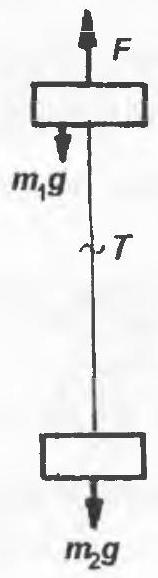
\includegraphics[max width=\textwidth, center]{2025_07_01_5b3ff9fa0d508c8e9f17g-217}

Fig. prob. 1.97 de urcare al primului corp. Înălțimea maximă la care ajunge primul corp este:

$$
h_{1 m}=h_{1}\left(t=t_{u}\right)=\frac{v_{01}^{2}}{2 g}=\frac{400}{20} \mathrm{~m}=20 \mathrm{~m}
$$

Din momentul în care primul corp a ajuns la înălțimea $h_{1 u}$, spațiile parcurse de cele două corpuri vor fi $h_{1}^{\prime}=\frac{g t^{2}}{2} ; h_{2}=v_{02} t-\frac{g t^{2}}{2}$. Timpul după care se\\
întâlnesc corpurile este dat de condiția: $h_{1}^{\prime}+h_{2}=h_{1 m}$ sau $\frac{g t^{2}}{2}+v_{02} t-\frac{g t^{2}}{2}=h_{1 m}$, de unde rezultă: $t=\frac{h_{1 m}}{v_{02}}=\frac{20}{10} \mathrm{~s}=2 \mathrm{~s}$.\\
1.99. Descompunem forța $F$ pe direcția\\
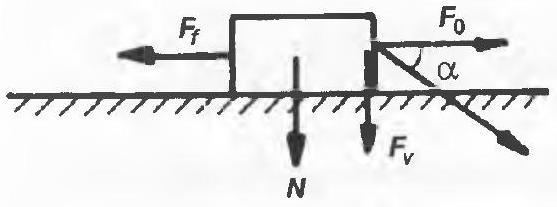
\includegraphics[max width=\textwidth, center]{2025_07_01_5b3ff9fa0d508c8e9f17g-218}

Fig. prob. 1.99 orizontală şi verticală (Fig. prob. 1.99): $F_{0}=F \cos \alpha ; F_{v}=F \sin \alpha$. Forța de apăsare normală pe planul orizontal este: $N=m g+F_{v}=m g+F \sin \alpha$, iar forța de frecare cu planul orizontal va fi:

$$
F_{f}=\mu N=\mu(m g+F \sin \alpha) .
$$

Pentru ca mişcarea să fie uniformă trebuie îndeplinită condiția: $F_{0}-F_{f}=0$; $F_{0}=F_{f} ; F_{\cos \alpha}=\mu(m g+F \sin \alpha)$, de unde rezultă: $\mu=\frac{F \cos \alpha}{m g+F \sin \alpha}$.\\
1.100. Conform enunțului, în cazul general forța de frecare poate fi scrisă sub forma: $F_{f}=b M^{\prime} g$ (1), unde $b$ este constanta de proportionalitate. La început mişcarea fiind uniformă, forța de tracțiune a trenului este $F_{t}=b M g$ (2), iar viteza trenului și a vagonului este $v_{0}$. După desprinderea de tren, vagonul merge uniform încetinit. Din $v=v_{0}-a_{1} t=0$, aflăm timpul de oprire $t_{0}=\frac{v_{0}}{a_{1}}$, iar din $m a_{1}=b m g$ rezultă $a_{1}=b g$ şi $t_{0}=\frac{\nu_{0}}{b g}(3)$. Spațiul parcurs de vagon până la oprire va fi: $d=v_{0} t_{0}-\frac{a_{1} t_{0}^{2}}{2}=\frac{v_{0}^{2}}{2 b g}$ (4). Accelerația trenului după desprinderea vagonului se află în felul următor:

$$
F_{t}-b(M-m) g=(M-m) a_{2} ; \quad \quad b M g-b M g+b m g=(M-m) a .
$$

Deci $a_{2}=\frac{b m g}{M-m}(5)$. Spațiul parcurs de tren până la oprirea vagonului este:

$$
D=v_{0} t_{0}+\frac{a_{2} t_{0}^{2}}{2}=v_{0} \cdot \frac{v_{0}}{2 b g}+\frac{1}{2} \cdot \frac{b m g}{M-m} \frac{v_{0}^{2}}{b^{2} g^{2}}=\frac{v_{0}^{2}}{2 b g} \cdot \frac{(2 M-2 m+m)}{(M-m)} .
$$

Deci: $D=d \frac{(2 M-m)}{M-m}$. Distanța dintre tren şi vagonul oprit va fi:

$$
x=D-d=\frac{2 M d-m d}{M-m}-d=\frac{2 M d-M d+m d}{M-m}
$$

Deci: $x=\frac{M}{M-m} d=11 \mathrm{~km}$.\\
1.101. Notăm cu $F_{c f}$ forța centrifugă şi cu $G$ greutatea aviatorului.\\
$v=720 \mathrm{~km} / \mathrm{h}=\frac{720 \cdot 10^{3}}{3600} \mathrm{~m} / \mathrm{s}=\frac{72}{36} \cdot 10^{2} \mathrm{~m} / \mathrm{s}=200 \mathrm{~m} / \mathrm{s}$.\\
Conform Fig. prob. 1.101, forța din enunțul problemei va ī in punctul inferior al cercului. Deci:\\
$F=F_{c f}+G=\frac{m v^{2}}{R}+m g=m\left(\frac{v^{2}}{R}+g\right)=70\left(\frac{4 \cdot 10^{4}}{8 \cdot 10^{2}}+10\right) \mathrm{N}=$ $=70\left(\frac{400}{8}+10\right) \mathrm{N}=4200 \mathrm{~N}$.\\
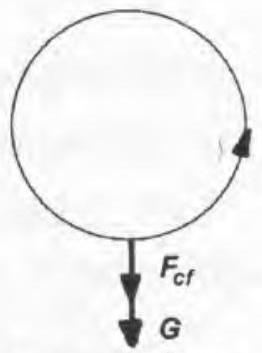
\includegraphics[max width=\textwidth, center]{2025_07_01_5b3ff9fa0d508c8e9f17g-219}

Fig. prob. 1.101\\
1.102. Aplicând legea conservării impulsului, viteza $v_{2}$ a corpului format se află în felul următor:

$$
m v_{1}=(m+M) \cdot v_{2} ; \quad v_{2}=\frac{m v_{1}}{m+M}=6 \mathrm{~m} / \mathrm{s}
$$

Energia cinetică a corpului format este:

$$
E=\frac{m+M}{2} v_{2}^{2}=9 \mathrm{~J}
$$

1.103. Conform Fig. prob. 1.103, greutatea $G$ a corpului se descompune în două componente: una paralelă cu planul $G_{p}$ şi alta normală pe plan $G_{n}$.

$$
\begin{aligned}
& G_{p}=G \sin \alpha=m g \sin \alpha ; \\
& G_{n}=G \cos \alpha=m g \cos \alpha
\end{aligned}
$$

Deoarece nu există frecare, componenta $G_{n}$ nu are nici o influență asupra mişcării. Din legea fundamentală a dinamicii: $-m g \sin \alpha=m a$, rezultă accelerația $a=-g \sin \alpha$ (1). Deci corpul va efectua de-a lungul planului o mişcare uniform încetinită. Conform formulei lui Galilei, viteza\\
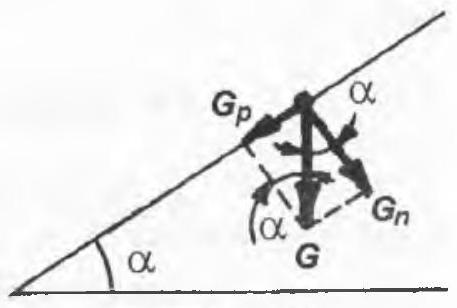
\includegraphics[max width=\textwidth, center]{2025_07_01_5b3ff9fa0d508c8e9f17g-219(1)}

Fig. prob. 1.103 corpului după ce parcurge o distanță $d$ va fi: $v=\sqrt{v_{0}^{2}-2 a d}$. În cazul nostru, când ajunge in punctul superior al planului viteza va fi: $\sqrt{v_{0}^{2}-2 g l \sin \alpha}=0$.

Deci: $v_{0}^{2}-2 g l \sin \alpha=0$ şi $v=\sqrt{2 g l \sin \alpha}=\sqrt{2 \cdot 10 \cdot 10 \cdot \frac{1}{2}}=10 \mathrm{~m} / \mathrm{s}$.\\
1.104. Scriem legea conservǎrii impulsului, înainte şi după ciocnirea plastică:\\
$m_{1} v_{1}=\left(m_{1}+m_{2}\right) \cdot u \Rightarrow u=\frac{m_{1} v_{1}}{m_{1}+m_{2}}=\frac{1000 \cdot 15}{2300}=6,52 \mathrm{~m} / \mathrm{s} ; \Delta E_{c}=E_{c f}-E_{c i}=$\\
$=\frac{\left(m_{1}+m_{2}\right) \cdot u^{2}}{2}-\frac{m_{1} v_{1}^{2}}{2}=\frac{1}{2} \frac{m_{1} m_{2}}{m_{1}+m_{2}} v_{1}^{2}=\frac{1}{2} \cdot \frac{1000 \cdot 1300}{2300} \cdot 15^{2}=63587 \mathrm{~J}$.\\
1.105. Răspuns corect $F$ ).\\
1.106. Răspuns corect $F$ ).\\
1.107. Pentru corpul $m_{1}: T-\mu m_{1} g=m_{1} a$; pentru $m_{2}: m_{2} g-T=m_{2} a$; adunăm relațiile: $m_{2} g-\mu m_{1} g=a\left(m_{1}+m_{2}\right)$, din care:

$$
\mu=\frac{m_{2}(g-a)-m_{1} a}{m_{1} g}=0,25 ; T=m_{2}(g-a)=15 \mathrm{~N} ; F_{S}=T \sqrt{2}=21 \mathrm{~N} .
$$

1.108. La ridicarea accelerată: $T-m g=m a$, din care:

$$
\begin{aligned}
& T=m(a+g)=65 \mathrm{~N} ; F_{\text {rupere }}=1,4 \mathrm{~T} ; F_{\text {rupere }}=m_{\max } g \text { (ridicare uniformă); } \\
& \Rightarrow m_{\max }=\frac{1,4 T}{g}=9,1 \mathrm{~kg}
\end{aligned}
$$

1.109. Forţa de atracție universală este forță centripetã $\frac{k m M}{r^{2}}=\frac{m v^{2}}{r}$, unde $r=R+h$ rezultă $\quad v=\sqrt{\frac{k M}{R+h}}$ dar $m g_{0}=\frac{k m M}{R^{2}}$ (la suprafața Pământului), deci:

$$
\begin{aligned}
& k M=g_{0} R^{2} \quad \text { şi } \quad v=R \sqrt{\frac{g_{0}}{R+h}}=\frac{R}{4} \sqrt{\frac{g_{0}}{R}}=2 \mathrm{~km} / \mathrm{s} \\
& T=\frac{2 \pi(R+h)}{v}=\frac{2 \pi \cdot 16 R \cdot 4}{\sqrt{g_{0} R}}=128 \pi \sqrt{\frac{R}{g_{0}}} \cong 90,3 \text { ore }
\end{aligned}
$$

1.110. Pentru a determina tendința de mişcare comparăm $G_{2}$ cu $G_{1 t}$; $G_{2}=m_{2} g=9 \mathrm{~N} ; G_{1 t}=m_{1} g \sin \alpha=3 \mathrm{~N} ; G_{2}>G_{1 t}$ deci $m_{1}$ urcă; $F_{\text {frecare }}$ în jos; $F_{f}=\mu m g \cos \alpha=1,5 \mathrm{~N} ; G_{2}>G_{1 t}+F_{f}$, deci mişcarea este accelerată:

$$
a=\frac{G_{2}-G_{1 t}-F_{f}}{m_{1}+m_{2}}=\frac{g\left(m_{2}-m_{1} \sin \alpha-\mu m_{1} \cos \alpha\right)}{m_{1}+m_{2}}=3 \mathrm{~m} / \mathrm{s}^{2} .
$$

Pentru corpul $m_{2}: m_{2} g-T=m_{2} a$ din care:

$$
T=m_{2}(g-a)=6,3 \mathrm{~N}
$$

1.111. $L_{\text {frecare }}=E_{c, f}-E_{c, i}=\frac{m v^{2}}{2}-\frac{m v_{0}^{2}}{2}=-0,64 \frac{m v_{0}^{2}}{2} \cong-4 \mathrm{~J}$.\\
1.112. Din Fig. prob. 1.112:

$$
\operatorname{tg} \alpha=\frac{F_{c f}}{G}=\frac{m \omega^{2} r}{m g}=\frac{\omega^{2} r}{g}
$$

unde $r=l \sin \alpha$ este raza cercului descris de corp; rezultă:

$$
\cos \alpha=\frac{g}{\omega^{2} l}=\frac{1}{2} ; \quad \alpha=60^{\circ} .
$$

1.113. Din legea conservării impulsului sistemului:\\
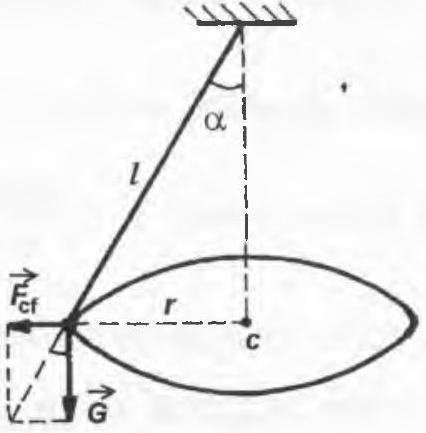
\includegraphics[max width=\textwidth, center]{2025_07_01_5b3ff9fa0d508c8e9f17g-221}

Fig. prob. 1.112\\
rezultă:

$$
m_{1} \vec{v}_{1}+m_{2} \vec{v}_{2}=\left(m_{1}+m_{2}\right) \vec{v}^{\prime}
$$

$$
v^{\prime}=\frac{m_{1} v_{1}-m_{2} v_{2}}{m_{1}+m_{2}}=-0,8 \mathrm{~m} / \mathrm{s}, \text { deci } \vec{v}^{\prime} \text { este orientată în sensul }
$$

vitezei $\vec{v}_{2}$;

$$
Q=\frac{1}{2} \cdot \frac{m_{1} m_{2}}{m_{1}+m_{2}}\left(v_{1}-v_{2}\right)^{2}=5,78 \mathrm{~J} .
$$

1.114. Componenta normală (la perete) pentru viteza mingii este: $v_{n}=v \sin \alpha$; în urma ciocnirii perfect elastice: $v_{n}^{\prime}=-v_{n}$, iar variaţia impulsului:

$$
\Delta p=m v_{n}^{\prime}-m v_{n}=-2 m v_{n}=-2 m v \sin \alpha ;
$$

forţa medie asupra mingii:

$$
F_{m}=\frac{|\Delta p|}{\Delta t}=\frac{2 m v \sin \alpha}{\Delta t}=5 \sqrt{3} \cdot 10^{-21} \mathrm{~N}=8,65 \cdot 10^{-21} \mathrm{~N} .
$$

1.115. Legea conservării impulsului sistemului: $m_{1} v=\left(m_{1}+m_{2}\right) v^{\prime}$; pentru mişcarea ce urmează ciocnirii aplicăm teorema variației energiei:

$$
\Delta E=L_{\text {neconservativ }} \Rightarrow E_{\text {final }}-E_{\text {initial }}=L_{\text {frecare }}
$$

dar

$$
E_{\text {final }}=\frac{k d^{2}}{2} ; E_{\text {initial }}=\frac{\left(m_{1}+m_{2}\right) v^{\prime 2}}{2} ; L_{\text {frecare }}=-\mu\left(m_{1}+m_{2}\right) g d ;
$$

obținem:

$$
v^{\prime 2}=\frac{k d^{2}}{m_{1}+m_{2}}+2 \mu g d ; v^{\prime}=0,7 \mathrm{~m} / \mathrm{s}
$$

apoi:

$$
v=\frac{\left(m_{1}+m_{2}\right) v^{\prime}}{m_{1}}=2,8 \mathrm{~m} / \mathrm{s} .
$$

1.116. Timpul de cădere este: $t_{c}=\sqrt{\frac{2 h}{g}}$; în acest timp discul trebuie să se rotească, la minim, cu $\alpha=6 \cdot \frac{2 \pi}{8}=\frac{3 \pi}{2}$ (unghiul dintre razele vectoare ale orificiile 1 şi 4); dar: $\alpha=\omega t_{c}$ şi $v=\frac{\omega}{2 \pi}$; in final $v_{\min }=\frac{3}{4} \sqrt{\frac{g}{2 h}}=\frac{\sqrt{3}}{4} \mathrm{rot} / \mathrm{s}$.\\
1.117. Ecuațiile de mişcare ale celor două corpuri sunt:

$$
y_{1}=v_{0} t-\frac{g t^{2}}{2} \quad \text { şi } \quad y_{2}=H-\frac{g t^{2}}{2} \text { (axa Oy orientată în sus); }
$$

condiția de întâlnire $y_{1}=y_{2} \Rightarrow t=\frac{H}{v_{0}}=5 \mathrm{~s}$ şi $y_{1}=y_{2}=h=75 \mathrm{~m}$.\\
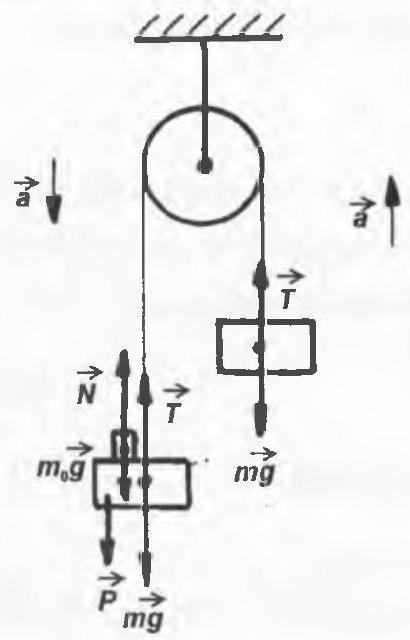
\includegraphics[max width=\textwidth, center]{2025_07_01_5b3ff9fa0d508c8e9f17g-222}

Fig. prob. 1.118\\
1.118. Asupra greutății din dreapta acționează forțele: $m \vec{g}, \vec{T}$-tensiunea în fir. Asupra sistemului din stânga acționează forțele: $m \vec{g}, \vec{T}$ şi $\vec{P}$-greutatea corpului $m_{0}$ (Fig. prob. 1.118).

Asupra corpului $m_{0}$ acţionează $m_{0} \vec{g}$ şi $\vec{N}$, reactiunea din partea lui $m$.

Ecuația de mişcare pentru corpuri proiectate pe direcția accelerației:

$$
\begin{aligned}
& T-m g=m a ; \quad m g+P-T=m a \\
& m_{0} g-N=m_{0} a \\
& P=N
\end{aligned}
$$

(pe baza legii a III-a a lui Newton) $\Rightarrow a=\frac{m_{0} g}{2 m+m_{0}}$.\\
1.119. Fie $v=$ viteza şalupei relativă la apă; $u=$ viteza de curgere a apei; $S=$ distanța dintre A şi B\\
$\Rightarrow S=(v+u) t_{1}-$ spațiul parcurs de şalupă în direcția de curgere a apei în timpul $t_{1}$\\
$S=(v-u) t_{2}-$ spațiul parcurs de şalupă în sens invers curgerii apei, în timpul $t_{2}$\\
$S=u \cdot t$ - spațiul parcurs de şalupă, dacă motorul este oprit.

$$
\begin{array}{ll}
u=\frac{S}{t} ; S=\left(v+\frac{S}{t}\right) \cdot t_{1} \Rightarrow v=\frac{S}{t_{1}}-\frac{S}{t} ; \quad S=\left(v-\frac{S}{t}\right) \cdot t_{2} \\
S=\left(\frac{S}{t_{1}}-\frac{S}{t}-\frac{S}{t}\right) \cdot t_{2} ; \\
t_{1} t=\left(t-2 t_{1}\right) \cdot t_{2} ; \\
t\left(t_{2}-t_{1}\right)=2 t_{1} t_{2} ; & t_{1} t-t t_{2}=-2 t_{1} t_{2} \\
t=\frac{2 t_{1} t_{2}}{t_{2}-t_{1}}
\end{array}
$$

1.120. Fie $t=$ timpul total de mişcare; $S_{1}=v_{1} \frac{t}{4}$ - spațiul parcurs în timpul $\frac{t}{4}$; $S_{2}=v_{2} \frac{3 t}{4}=$ drumul parcurs în restul timpului $\frac{3 t}{4}$.\\
$v_{\text {med }}=\frac{\operatorname{def}}{t}=\frac{S_{1}+S_{2}}{t}=\frac{v_{1} \frac{t}{4}+v_{2} \frac{3 t}{4}}{t}=\frac{v_{1}+3 v_{2}}{4}=\frac{7+3 \cdot 4}{4}=\frac{19}{4}=4,75 \mathrm{~km} / \mathrm{h}$.\\
$S_{1}=\frac{S}{4}-$ drumul parcurs cu viteza $v_{1}$;\\
$S_{2}=\frac{3 S}{4}-$ drumul parcurs cu viteza $v_{2} \Rightarrow t_{1}=\frac{S_{1}}{v_{1}}=\frac{S}{4 v_{1}} ; \quad t_{2}=\frac{S_{2}}{v_{2}}=\frac{3 S}{4 v_{2}} ;$\\
$v_{\text {med }}=\frac{S_{1}+S_{2}}{t_{1}+t_{2}}=\frac{S}{\frac{S}{4 v_{1}}+\frac{3 S}{4 v_{2}}}=\frac{4 v_{1} v_{2}}{v_{2}+3 v_{1}}=4,48 \mathrm{~km} / \mathrm{h}$.\\
1.121. $m=0,2 \mathrm{~kg} ; h=1 \mathrm{~m} ; a=8 \mathrm{~m} / \mathrm{s}^{2} ; \Delta p=$ ? (Fig. prob. 1.121)\\
$v_{f}^{2}=2 a h \Rightarrow v_{f}=\sqrt{2 a h}=\sqrt{2 \cdot 8 \cdot 1}=\sqrt{16}=4 \mathrm{~m} / \mathrm{s}$.\\
$\Delta p=p_{f}-p_{i}=m v_{f}-m v_{i}=m v_{f}=0,2 \cdot 4=0,8 \mathrm{~kg} \mathrm{~m} / \mathrm{s}$, deoarece $m v_{i}=0$.\\
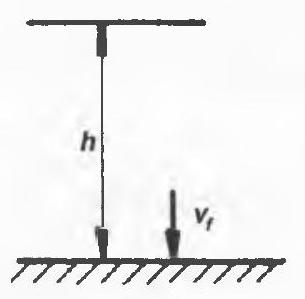
\includegraphics[max width=\textwidth, center]{2025_07_01_5b3ff9fa0d508c8e9f17g-223}

Fig. prob. 1.121\\
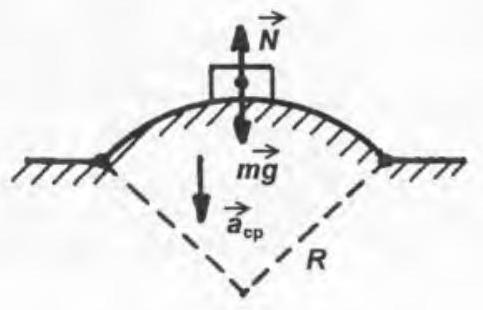
\includegraphics[max width=\textwidth, center]{2025_07_01_5b3ff9fa0d508c8e9f17g-223(1)}

Fig. prob. 1.122\\
1.122. Ecuația de mişcare în punctul superior al podețului este (Fig. prob. 1.122):

$$
m g-N=m a_{c p}=\frac{m v^{2}}{R} ; \quad N=\frac{m g}{2}(\text { condiția problemei })
$$

Rezultă: $R=\frac{2 v^{2}}{g}=\frac{2}{10} \cdot 20^{2}=\frac{400}{5}=80 \mathrm{~m}$.\\
1.123. Se aplică teorema de variație a energiei mecanice $E_{2}-E_{1}=L$ (lucrul mecanic al forțelor neconservative) (Fig. prob. 1.123). $E_{2}=\frac{m v_{f}^{2}}{2}$ şi $E_{1}=\frac{m v_{0}^{2}}{2}+m g h$. Rezultă $\frac{m v_{f}^{2}}{2}-\left(\frac{m v_{0}^{2}}{2}+m g h\right)=L$.\\
$L=-220 \mathrm{~J}$.\\
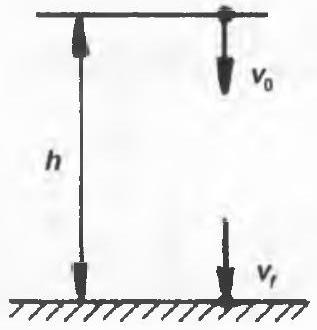
\includegraphics[max width=\textwidth, center]{2025_07_01_5b3ff9fa0d508c8e9f17g-224}

Fig. prob. 1.123\\
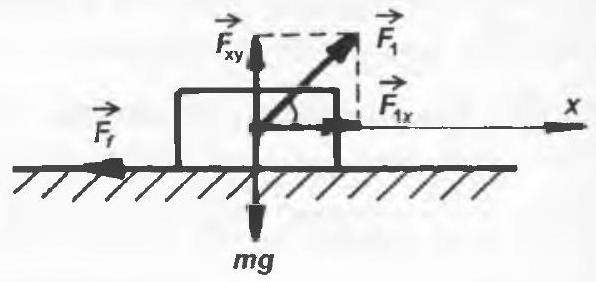
\includegraphics[max width=\textwidth, center]{2025_07_01_5b3ff9fa0d508c8e9f17g-224(1)}

Fig. prob. 1.124\\
1.124. (Fig. prob. 1.124) Ox: $F_{1} \cos \alpha-F_{f}=0 ; \quad(v=$ const. $) \quad(a=0)$

$$
\begin{aligned}
& F_{f}=\mu N=\mu\left(m g-F_{1} \sin \alpha_{1}\right) \\
& F_{1} \cos \alpha_{1}=\mu\left(m g-F_{1} \sin \alpha_{1}\right)
\end{aligned}
$$

analog: $\quad F_{2} \cos \alpha_{2}=\mu\left(m g-F_{2} \sin \alpha_{2}\right)$\\
Rezultă: $\quad \frac{F_{1}}{F_{2}} \frac{\cos \alpha_{1}}{\cos \alpha_{2}}=\frac{m g-F_{1} \sin \alpha_{1}}{m g-F_{2} \sin \alpha_{2}}$\\
$\Rightarrow m=\frac{1}{g} \frac{F_{1} F_{2}\left(\sin \alpha_{2} \cos \alpha_{1}-\cos \alpha_{2} \sin \alpha_{1}\right)}{F_{1} \cos \alpha_{1}-F_{2} \cos \alpha_{2}} \Rightarrow m=20 \sqrt{3} \mathrm{~kg}$.\\
1.125. a) $\frac{m v_{f}^{2}}{2}+Q=\frac{m v_{0}^{2}}{2} \Rightarrow m v_{f}^{2}+2 Q=m v_{0}^{2} \Rightarrow$

$$
v_{f}=\sqrt{\frac{m v_{0}^{2}-2 Q}{m}}=\sqrt{v_{0}^{2}-\frac{2}{m} Q}=100 \mathrm{~m} / \mathrm{s}
$$

b) $v_{f}^{2}=v_{0}^{2}+2 a l \Rightarrow a=-4 \mathrm{~m} / \mathrm{s}^{2}$\\
c) $v_{f}=v_{0}+a t \Rightarrow t=\frac{v_{f}-v_{0}}{a}=50 \mathrm{~s}$.\\
1.126. Pentru bătaie, avem relația (Fig. prob. 1.126):\\
$d=v_{0} \sqrt{\frac{2 h}{g}}$\\
Avem: $h=l \sin \alpha ; d=l \cos \alpha$\\
Obținem:\\
$v_{0}=\cos \alpha \sqrt{\frac{g l}{2 \sin \alpha}}$\\
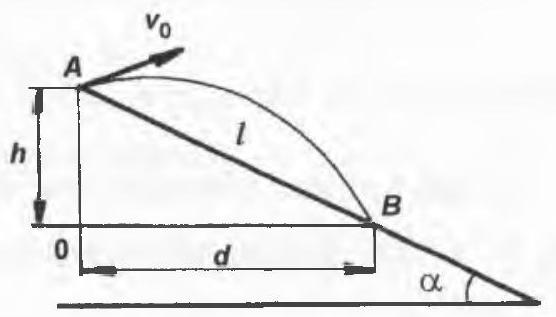
\includegraphics[max width=\textwidth, center]{2025_07_01_5b3ff9fa0d508c8e9f17g-225(1)}

Fig. prob. 1.126\\
și înlocuind numeric $v_{0}=15 \mathrm{~ms}^{-1}$.\\
1.127. Procedăm la izolarea sistemului de legături (vezi Fig. prob. 127.a):

Caz 1.\\
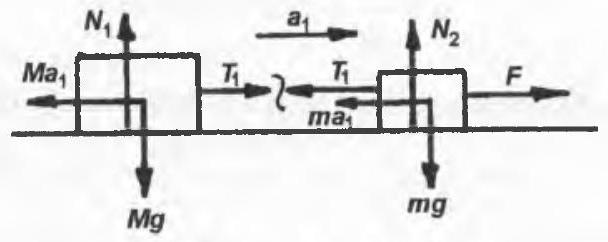
\includegraphics[max width=\textwidth, center]{2025_07_01_5b3ff9fa0d508c8e9f17g-225}

Fig. prob. 127.a\\
Avem: $\left\{\begin{array}{l}F-T_{1}-m a_{1}=0 \\ T_{1}-M a_{1}=0\end{array} \Rightarrow a_{1}=\frac{1}{M+m} F ; \quad T_{1}=\frac{M}{M+m} F\right.$.\\
Caz 2. (vezi Fig. prob. 127.b)\\
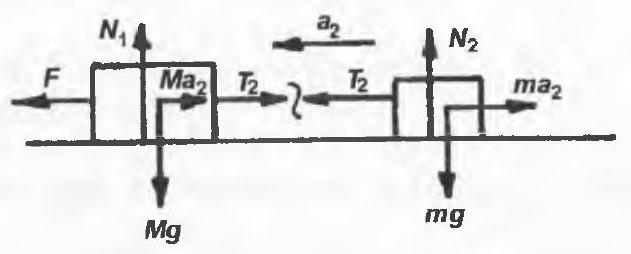
\includegraphics[max width=\textwidth, center]{2025_07_01_5b3ff9fa0d508c8e9f17g-225(2)}

Fig. prob. 127.b\\
$\left\{\begin{array}{l}T_{2}-m a_{2}=0 \\ F-T_{2}-M a_{2}=0\end{array} \Rightarrow a_{2}=\frac{1}{M+m} F ; \quad T_{2}=\frac{m}{M+m} F\right.$

Cum $M>m$, rezultă $a_{1}=a_{2}$ şi $T_{1}>T_{2}$.\\
1.128. Notând cu $x_{1}$ şi $x_{2}$ alungirile resorturilor legate în serie, avem:\\
$E_{1}=\frac{k_{1} x_{1}^{2}}{2}=\frac{k_{1}^{2} x_{1}^{2}}{2 k_{1}}=\frac{\left(k_{1} x_{1}\right)^{2}}{2 k_{1}}=\frac{F_{1}^{2}}{2 k_{1}}$ şi analog $E_{2}=\frac{F_{2}^{2}}{2 k_{2}}$.\\
În cazul legării în serie forțele ce acționează asupra resorturilor sunt egale:

$$
F_{1}=F_{2}=F \Rightarrow \frac{E_{1}}{E_{2}}=\frac{k_{2}}{k_{1}}
$$

1.129. Aplicăm sistemului conservarea impulsului

$$
m \cdot 0=M \cdot 0=m u+M v \Rightarrow v=\frac{m}{M} u
$$

Spațiul până la oprire $\Rightarrow S=\frac{V^{2}}{2 \mu g}=\frac{m^{2} u^{2}}{2 M^{2} \mu g}=50 \mathrm{~m}$.\\
1.130. Viteza corpul este de forma $v=m+n t^{2}=0,18 \mathrm{~m} / \mathrm{s}$.

Acceleraţia corpului este de forma:

$$
a=\frac{\mathrm{d} v}{\mathrm{~d} t}=2 n t=0,08 \mathrm{~m} / \mathrm{s}^{2}
$$

1.131. În primele 5 s mişcarea este uniform accelerată, deci:

$$
s=\frac{1}{2} a t^{2} \Rightarrow a=\frac{2 s}{t^{2}}=6 \mathrm{~m} / \mathrm{s}^{2}
$$

Viteza după primele 5 s este $v=a t=30 \mathrm{~m} / \mathrm{s}$. În următoarele 5 s mişcarea este uniformă, $F=0$, deci $s=v t=150 \mathrm{~m}$.\\
1.132. Electronul se mişcă uniform accelerat fără viteză inițială, $v_{0}=0$, adică $v^{2}=2 a s \Rightarrow a=\frac{v^{2}}{2 s}$. Forța de accelerație este:

$$
F=m a=m \frac{v^{2}}{2 s}=1,62 \cdot 10^{-15} \mathrm{~N}
$$

1.133. În primele 2 s corpul se deplasează cu accelerația $a=2 \mathrm{~m} / \mathrm{s}^{2}, \operatorname{dec}$ spațiul parcurs în acest timp este $s_{1}=\frac{a t^{2}}{2}=4 \mathrm{~m}$. După $t=2 \mathrm{~s}$ avem:

$$
T=m\left(g+a^{\prime}\right) \Rightarrow a^{\prime}=\frac{T-m g}{m}=0 \mathrm{~m} / \mathrm{s}^{2}
$$

deci corpul se deplasează uniform, cu viteză constantă egală cu $\nu=a t=4 \mathrm{~m} / \mathrm{s}$.\\
Spațiul parcurs în timpul $t_{2}=5 \mathrm{~s}-2 \mathrm{~s}=3 \mathrm{~s}$ este $s_{2}=v t_{2}==12 \mathrm{~m}$.\\
Spațiul total parcurs de corp va fi $s=s_{1}+s_{2}=16 \mathrm{~m}$.\\
1.134. Timpul de coborâre a obiectului este $t_{c}=\sqrt{\frac{2 y}{g}}=19,49 \mathrm{~s}$.

Componentele vitezei vor fi $v_{x}=v=90 \mathrm{~m} / \mathrm{s}$, componenta după axa $\mathrm{O} x$, iar $v_{y}=g t_{c}=194,9 \mathrm{~m} / \mathrm{s}$, componenta după axa $\mathrm{O} y$.\\
1.135. Energia mecanică a corpului este $E=E_{c}+E_{p}$ unde $E_{c}$ este energie cinetică a corpului, iar $E_{p}$ este energia potentială a corpului.

Energia cinetică este $E_{c}=\frac{m v^{2}}{2}$ unde $v$ este viteza la înălțimea de 10 m , adică $v=\sqrt{2 g\left(h-h_{1}\right)}=20 \sqrt{2} \mathrm{~m} / \mathrm{s}$.

Înlocuind se obține $E_{c}=800 \mathrm{~J}$. Energie potențială este $E_{p}=m g h_{1}=200 \mathrm{~J}$.\\
Energia totală va fỉ $E=1000 \mathrm{~J}$.\\
1.136. Conform Fig. prob. 1.136 :

$$
F=m(g+a)=2(9,8+1,2)=22 \mathrm{~N} .
$$

1.137. $F=\left(m_{1}+m_{2}\right) a ; f=m_{2} a$.

$$
f=\frac{m_{2}}{m_{1}+m_{2}}=50 \frac{2}{8+2}=10 \mathrm{~N}
$$

\begin{center}
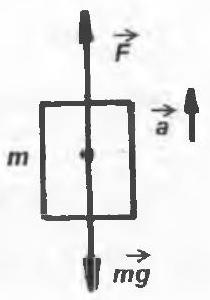
\includegraphics[max width=\textwidth]{2025_07_01_5b3ff9fa0d508c8e9f17g-227(1)}
\end{center}

Fig. prob. 1.136\\
1.138. $d_{1}=v_{01} t_{1}+\frac{a t_{1}^{2}}{2}$; $d_{2}=v_{02} t_{2}+\frac{a t_{2}^{2}}{2} ; v_{02}=v_{01}+a t_{1} \quad ; \quad d_{1}=d_{2}=\frac{d}{2} ; a=d \frac{t_{1}-t_{2}}{t_{1} t_{2}\left(t_{1}+t_{2}\right)}=0,25 \mathrm{~m} / \mathrm{s}^{2}$.\\
1.139. $t_{u}=t_{c}=t / 2 ; h=\frac{g t^{2}}{8}=4,9 \mathrm{~m}$.\\
1.140. Vezi Fig. prob. 1.140.\\
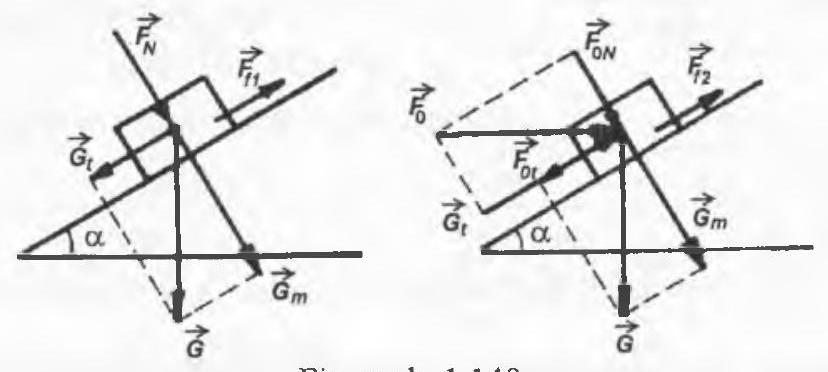
\includegraphics[max width=\textwidth, center]{2025_07_01_5b3ff9fa0d508c8e9f17g-227}

Fig. prob. 1.140

$$
\begin{aligned}
& F_{f_{1}}=\mu\left(F_{N}+G \cos \alpha\right) ; \quad G_{t}=G \sin \alpha \\
& F_{f_{2}}=\mu\left(F_{0} \sin \alpha+G \cos \alpha\right) ; \quad F_{t}=G \sin \alpha-F_{0} \cos \alpha \\
& \left\{\begin{array}{l}
\mu\left(F_{N}+G \cos \alpha\right)=G \sin \alpha \\
\mu\left(F_{0} \sin \alpha+G \cos \alpha\right)=G \sin \alpha-F_{0} \cos \alpha
\end{array}\right. \\
& n=\frac{F_{N}}{F_{0}} \\
& \mu=\frac{\cos \alpha}{n-\sin \alpha}=\frac{1}{2 \sqrt{2}-1} .
\end{aligned}
$$

1.141. $\mu m g=\frac{m v^{2}}{R} \Rightarrow \mu=\frac{v^{2}}{R g}=\frac{10^{2}}{50 \cdot 9,8}=0,2$.\\
1.142. $P=F \cdot v=m g \frac{h}{t} \Rightarrow t=\frac{m g h}{P}=\frac{500 \cdot 9,8 \cdot 18}{9,8 \cdot 10^{3}}=0,9 \mathrm{~s}$.\\
1.143. $-F=m a=m \frac{\nu}{t} \Rightarrow|F|=\frac{4009 \cdot 10^{3} \cdot 10}{20}=200 \mathrm{kN}$.\\
1.144. Viteza instantanee a mobilului este $v=v_{0}+a t ; v_{0}=3 \mathrm{~m} / \mathrm{s}$, $a=8 \mathrm{~m} / \mathrm{s}, v=8 t+3$. La $t=3 \mathrm{~s} \Rightarrow v(3)=8 \cdot 3+3=27 \mathrm{~m} / \mathrm{s}$.\\
1.145. Din formula lui Galilei pe planul înclinat, respectiv orizontal, avem:

$$
\begin{aligned}
& 0=v_{0}^{2}-2 a_{u} l, \\
& 0=v_{0}^{2}-2 a_{0} l,
\end{aligned}
$$

unde $a_{u}$ este accelerația la urcarea pe plan și $a_{0}$ accelerația pe planul orizontal.\\
Rezultã $a_{u}=a_{0} \Rightarrow g(\sin \alpha+\mu \cos \alpha)=g \mu$

$$
\mu(1-\cos \alpha)=\sin \alpha .
$$

Ținând cont de definiția unghiului de frecare, avem:

$$
\mu=\operatorname{tg} \varphi=\frac{\sin \alpha}{1-\cos \alpha}=\frac{2 \sin \frac{\alpha}{2} \cos \frac{\alpha}{2}}{2 \sin ^{2} \frac{\alpha}{2}} \Rightarrow \operatorname{tg} \varphi=\frac{\cos \frac{\alpha}{2}}{\sin \frac{\alpha}{2}}=\operatorname{ctg} \frac{\alpha}{2}=\operatorname{tg}\left(\frac{\pi}{2}-\frac{\alpha}{2}\right) .
$$

Rezultă $\varphi=\frac{\pi-\alpha}{2}$.\\
1.146. $\frac{m v_{1}^{2}}{2}=\frac{1}{n} \frac{m v_{0}^{2}}{2} \Rightarrow v_{1}=\frac{v_{0}}{\sqrt{n}}$.

Pe directia $O x$ mişcarea este uniformă, componenta vitezei pe această axă fiind tot timpul constantă (Fig. prob. 1.146).

$$
v_{0} \cos \alpha=v_{1} \cos \beta \Rightarrow \cos \beta=\sqrt{n} \cos \alpha
$$

\begin{center}
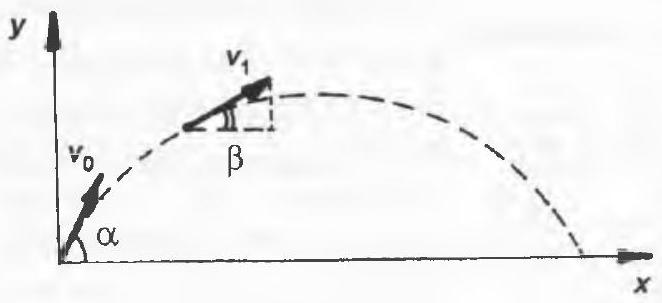
\includegraphics[max width=\textwidth]{2025_07_01_5b3ff9fa0d508c8e9f17g-229}
\end{center}

Fig. prob. 1.146\\
1.147. Fie $v_{0}=0, v_{1}, v_{2}$ şi $v_{3}$ vitezele corpului în punctele de abscise $x=0, x_{1}=2 \mathrm{~m}, x_{2}=6 \mathrm{~m}$, respectiv $x_{3}=8 \mathrm{~m}$.

Conform teoremei variației energiei cinetice avem (Fig. prob. 1.147):

$$
\left.\begin{array}{l}
\frac{m v_{1}^{2}}{2}=L_{1} \\
\frac{m v_{2}^{2}}{2}-\frac{m v_{1}^{2}}{2}=L_{2} \\
\frac{m v_{3}^{2}}{2}-\frac{m v_{2}^{2}}{2}=L_{3}
\end{array}\right\} \Rightarrow \frac{m v_{3}^{2}}{2}=L_{1}+L_{2}+L_{3}
$$

unde $L_{1}=\frac{2 \cdot 27}{2} \mathrm{~J}=27 \mathrm{~J}$;\\
$L_{2}=(6-2) \cdot 27 \mathrm{~J}=108 \mathrm{~J}$ şi $L_{3}=\frac{(8-6) \cdot 27}{2} \mathrm{~J}=27 \mathrm{~J}$.\\
Rezultă $v_{3}=\sqrt{\frac{2\left(L_{1}+L_{2}+L_{3}\right)}{m}}=\sqrt{\frac{2 \cdot 162}{1}}=18 \mathrm{~m} / \mathrm{s}$.\\
1.148. Conform Fig. prob. 1.148 , vitezele cu care corpurile ajung în punctul cel mai de jos al suprafeței cilindrice sunt $v_{1}=v_{2}=v=\sqrt{2 g R}$.

Energia potențială inițială este

$$
E_{p}=\left(m_{1}+m_{2}\right) g R=(n+1) m_{1} R g .
$$

\begin{center}
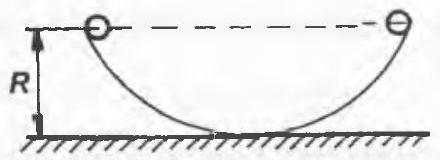
\includegraphics[max width=\textwidth]{2025_07_01_5b3ff9fa0d508c8e9f17g-229(1)}
\end{center}

Fig. prob. 1.148

Căldura degajată în urma ciocnirii plastice este:

$$
Q=\frac{1}{2} \cdot m_{r} \cdot v_{r}^{2}=\frac{1}{2} \cdot \frac{m_{1} m_{2}}{m_{1}+m_{2}} \cdot(2 v)^{2}=\frac{1}{2} \cdot \frac{n m_{1}^{2}}{(n+1) m_{1}} \cdot 4 \cdot 2 \cdot R g=\frac{4 n m_{1} R g}{(n+1)} .
$$

Ea reprezintă fracțiunea $f$ din energia potențială inițială:

$$
f=\frac{Q}{E_{p}}=\frac{4 n m_{1} R g}{(n+1)} \cdot \frac{1}{(n+1) m_{1} R g}=\frac{4 n}{(n+1)^{2}}
$$

1.149. Viteza cu care corpul de masă $m$ va ciocni plastic corpul atâmat\\
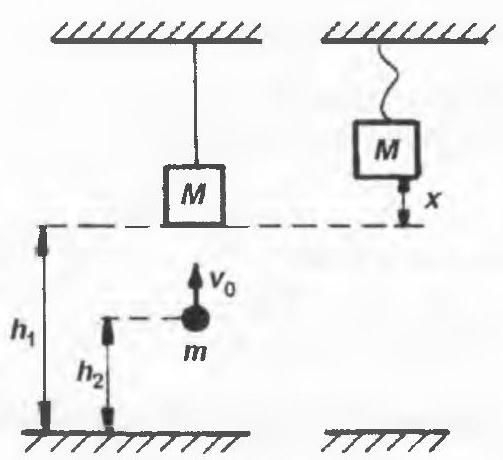
\includegraphics[max width=\textwidth, center]{2025_07_01_5b3ff9fa0d508c8e9f17g-230}

Fig. prob. 1.149 (Fig. prob. 1.149) este:


\begin{equation*}
v^{2}=v_{0}^{2}-2 g\left(h_{1}-h_{2}\right) . \tag{1}
\end{equation*}


Din conservarea impulsului în ciocnirea plastică, rezultă:


\begin{equation*}
m v=(m+M) \cdot V \Rightarrow V=\frac{m}{m+M} \cdot v \tag{2}
\end{equation*}


Distanța pe care se ridică cele două corpuri se găseşte din ecuația lui Galilei:

$$
0=V^{2}-2 g x \Rightarrow x=\frac{V^{2}}{2 g}
$$

Folosind relația (2) se obține:

$$
x=\left(\frac{m}{m+M}\right)^{2}\left(\frac{v_{0}^{2}}{2 g}-h_{1}+h_{2}\right) .
$$

1.150. Caracteristicile mişcării primei castane în momentul aruncării cele de-a doua castane:

$$
\begin{aligned}
& x_{10}=\frac{1}{2} g t^{2}=\frac{1}{2} \cdot 9,8 \cdot 1^{2}=4,9 \mathrm{~m} \\
& v_{10}=g t=9,8 \cdot 1=9,8 \mathrm{~m} / \mathrm{s} .
\end{aligned}
$$

Ecuațiile de mişcare pentru cele două castane sunt:

$$
\begin{aligned}
& x_{1}=x_{10}+v_{10} t+\frac{1}{2} g t^{2} \\
& x_{2}=v_{20} t+\frac{1}{2} g t^{2} .
\end{aligned}
$$

Condiția de întâlnire a celor două castane este:

$$
x_{1}=x_{2} \Rightarrow x_{10}+v_{10}+\frac{1}{2} g t^{2}=v_{20}+\frac{1}{2} g t^{2} .
$$

Rezolvând în raport cu timpul $t$ rezultă:

$$
t=\frac{x_{10}}{v_{20}-v_{10}}=\frac{4,9}{15-9,8}=0,94 \mathrm{~s} .
$$

Distanța parcursă se obţine înlocuind valoarea timpului în una din ecuațiile de mişcare:

$$
x_{1}=4,9+9,8 \cdot 0,94+\frac{1}{2} \cdot 9,8 \cdot 0,94^{2}=18,4 \mathrm{~m} .
$$

1.151. Diagrama forțelor care acționează asupra corpului este reprezentată în Fig. prob. 1.151. Descompunem forțele care acționează asupra corpului de-a lungul planului (axa $\mathrm{O} x$ ) şi pe direcţie perpendiculară (axa $\mathrm{O} y$ ). Conform principiului fundamental al mecanicii, accelerația este determinatã de rezultanta forțelor care acționează asupra corpului. Deoarece corpul urcă de-a lungul planului, accelerația este îndreptată pe direcția $\mathrm{O} x$.

$$
\begin{array}{ll}
\mathrm{O} x: & F \cos \theta-G \sin \theta-f=m a \\
\mathrm{O} y: & N-G \cos \theta-F \sin \theta=0 .
\end{array}
$$

\begin{center}
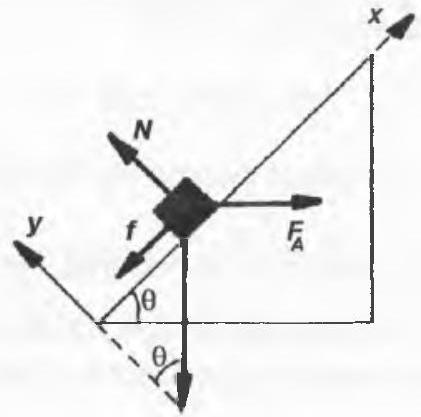
\includegraphics[max width=\textwidth]{2025_07_01_5b3ff9fa0d508c8e9f17g-231}
\end{center}

Fig. prob. 1.151

Forța de frecare este:

$$
f=\mu \cdot N .
$$

Rezolvând sistemul celor trei ecuații se obține:

$$
F \cos \theta-G \sin \theta-\mu(G \cos \theta+F \sin \theta)=m a
$$

adică $F=m \cdot \frac{a+g(\sin \theta+\mu \cos \theta)}{\cos \theta-\mu \sin \theta}$.\\
Înlocuind valorile numerice se obține valoarea acestei forțe:

$$
F=10 \cdot \frac{\frac{\sqrt{2}}{2}+10 \cdot\left(\frac{\sqrt{2}}{2}+0,2 \cdot \frac{\sqrt{2}}{2}\right)}{\frac{\sqrt{2}}{2}-0,2 \cdot \frac{\sqrt{2}}{2}}=162,5 \mathrm{~N} .
$$

1.152. Conform principiului fundamental al mecanicii:


\begin{align*}
& F=m_{1} a_{1}  \tag{1}\\
& F=m_{2} a_{2} . \tag{2}
\end{align*}


Deoarece $a_{2}=2 a_{1}$, se obține:


\begin{equation*}
m_{1} a_{1}=2 m_{2} a_{1} \Rightarrow m_{1}=2 m_{2} . \tag{3}
\end{equation*}


Dacă se lipesc cele două mase, forța $F$ va produce accelerația $a$ determinată din ecuația:


\begin{equation*}
F=\left(m_{1}+m_{2}\right) a . \tag{4}
\end{equation*}


Adunând relațiile (1), (2) şi folosind (4) rezultă:

$$
2\left(m_{1}+m_{2}\right) a=m_{1} a_{1}+m_{2} a_{2}
$$

de unde, cu ajutorul relației (3) se obține: $a=\frac{2 m_{2} a_{1}+m_{2} 2 a_{1}}{2\left(2 m_{2}+m_{2}\right)}=\frac{2}{3} a_{1}$.\\
1.153. Din legea de conservare a impulsului în ciocnirea plastică dintre cele două vehicule, rezultă:

$$
M v=(M+m) V \Rightarrow V=\frac{M}{M+m} v=12 \mathrm{~m} / \mathrm{s}
$$

Folosind ecuația lui Galilei:


\begin{equation*}
0=V^{2}-2 a x \Rightarrow x=\frac{V^{2}}{2 a} \tag{1}
\end{equation*}


Accelerația se determină din principiul fundamental al mecanicii, singura forță care determină accelerația fiind forța de frecare:

$$
\mu m g=m a \Rightarrow a=\mu g=0,2 \cdot 10=2 \mathrm{~m} / \mathrm{s}^{2} .
$$

Înlocuind (1) în (2) se obține:

$$
x=\frac{V^{2}}{2 \mu g}=36 \mathrm{~m}
$$

1.154. Scriem conservarea impulsului şi a energiei cinetice pentru sistemul format din cele două particule:

$$
\begin{aligned}
& 4 v M-m v=m v_{1} \\
& \frac{M(4 v)^{2}}{2}+\frac{m v^{2}}{2}=\frac{m v_{1}^{2}}{2} .
\end{aligned}
$$

Ridicăm la pătrat prima ecuație, o împărţim la cea de-a doua şi obținem:

$$
M / m=1,5 .
$$

1.155. Scriem conservarea impulsului pentru cea de-a doua barcă, la care se adaugă masa $m$ :

$$
m_{2} v-m v=\left(m_{2}+m\right) v_{2},
$$

de unde se obține

$$
m_{2}=m \frac{v+v_{2}}{v-v_{2}}=100 \mathrm{~kg} .
$$

1.156. Descompunând mişcarea după direcţia verticală şi orizontală, se obține:

$$
h=\frac{g t_{\mathrm{c}}^{2}}{2} \text { şi } k h=v \cdot t_{\mathrm{c}} \text {, de unde } v=k \sqrt{\frac{g h}{2}} \text {. }
$$

1.157. Ţinând cont de faptul că la baza planului înclinat corpul suferă o ciocnire perfect elastică și că forta de frecare conduce la disiparea energiei mecanice, scriem că variația energiei mecanice este egală cu lucrul mecanic al forței de frecare:

$$
m g h_{1}-m g h=-\mu m g \cos \alpha\left(l_{1}+l_{2}\right) .
$$

Dar $l_{1}=\frac{h}{\sin \alpha}$ şi $l_{2}=\frac{h_{1}}{\sin \alpha}$, de unde, înlocuind în ecuația de mai sus, se obține:

$$
h_{1}=h \frac{1-\mu \operatorname{ctg} \alpha}{1+\mu \operatorname{ctg} \alpha}=8 \mathrm{~m} .
$$

1.158. Variația impulsului mingii este egal cu impulsul forței de impact, deci $2 m v \cos \alpha=F \cdot \Delta t$, de unde $F=\frac{2 m v \cos \alpha}{\Delta t}=2500 \mathrm{~N}$.\\
1.159. Scriind condiția de stabilitate a Pământului pe traiectoria sa presupusă circulară, adică forța de atracție gravitațională este egală cu forța centrifugă, $k \frac{m M}{R^{2}}=\frac{m v^{2}}{R}$, se obţine $M=\frac{v^{2} R}{k} \cong 2 \cdot 10^{32} \mathrm{~kg}$.\\
1.160. Răspuns corect: $C$ ).\\
1.161. Răspuns corect: C ).\\
1.162. Viteza pe care o are primul corp, cel care cade liber, înaintea procesului de ciocnire este $v_{1}=g t_{1}=40 \mathrm{~m} / \mathrm{s}$, iar înălțimea la care de petrece această ciocnire este $h_{1}=\frac{g}{2} t_{1}^{2}=80 \mathrm{~m}$.

După ciocnire, corpul nou format va avea o viteză orizontală şi una verticală, obținute din conservarea impulsului,

$$
\begin{aligned}
& m_{1} v_{1}=\left(m_{1}+m_{2}\right) v_{\text {vert }} \\
& m_{2} v_{2}=\left(m_{1}+m_{2}\right) v_{\text {oriz. }}
\end{aligned}
$$

Dar $m_{1}=m_{2}$, de unde $v_{\text {vert. }}=20 \mathrm{~m} / \mathrm{s}$ şi $v_{\text {oriz. }}=10 \mathrm{~m} / \mathrm{s}$. Timpul în care corpul ajunge pe pământ este obținut din ecuația $h-h_{1}=v_{\text {vert }} t+\frac{g}{2} t^{2}$, care are soluția $t=2(\sqrt{2}-1)$, de unde spațiul parcurs pe orizontală este

$$
d=v_{\text {oriz. }} t=8,2 \mathrm{~m}
$$

1.163. Dacă notănt cu $r$ raza cercului pe care se mişcă motocicliştii, cu $\omega_{1}$ şi $\omega_{2}$ vitezele lor unghiulare, spațiile $s_{1}$ şi $s_{2}$ parcurse in timpul $T$ sunt date de relațiile:

$$
s_{1}=r \omega_{1} T ; s_{2}=r \omega_{2} T
$$

Pentru ca primul motociclist să-l prindă pe al doilea din urmă, trebuie ca

$$
s_{1}=s_{2}+2 \pi r
$$

Se obține imediat că $T=\frac{2 \pi}{\omega_{1}-\omega_{2}}$, numărul de rotații efectuat de primul motociclist şi de cel de-al doilea fiind

$$
\begin{aligned}
& n_{1}=\frac{r \omega_{1} T}{2 \pi r}=\frac{\omega_{1}}{\omega_{1}-\omega_{2}}=\frac{v_{1}}{v_{1}-v_{2}}=5 \text { şi } \\
& n_{2}=\frac{r \omega_{2} T}{2 \pi r}=\frac{\omega_{2}}{\omega_{1}-\omega_{2}}=\frac{v_{2}}{v_{1}-v_{2}}=4 .
\end{aligned}
$$

1.164. Ciocnirea bilei cu planul este însoțită de o disipare a energiei sale cinetice $\frac{m v_{1}^{2}}{2}<\frac{m v_{0}^{2}}{2} \Rightarrow e<1$.

Fie $v_{n-1}$ şi $v_{n}$ vitezele bilei înainte şi imediat după cea de-a $n$-a ciocnire. Ele sunt legate prin relația din enunțul problemei $v_{n}=e v_{n-1}, e$ se numeşte coeficient de restituire. Energia cinetică $\frac{m v_{n}^{2}}{2}$ produce ridicarea bilei până la o înălțime $h_{n}$, astfel încât

$$
\begin{aligned}
& m g h_{n}=\frac{m v_{n}^{2}}{2}, \text { de unde rezultă } \\
& \frac{h_{n}}{h_{n-1}}=\frac{v_{n}^{2}}{v_{n-1}^{2}}=e^{2}, \Rightarrow h_{n}=h_{n-1} e^{2}
\end{aligned}
$$

Deci înălțimile maxime succesive atinse de bilă sunt:

$$
h_{0}, h_{1}=h_{0} e^{2}, h_{2}=h_{0} e^{4}, \ldots \ldots, h_{n}=h_{0} e^{2 n}, \ldots
$$

Atunci când bila se intoarce în sus cu viteza $v_{n}$ viteza ei scade după legea $v=v_{n}-g t$ şi se anulează pentru $t=\frac{v_{n}}{g}$. Deci durata celei de-a $n$-a ridicări şi coborâri este $\theta_{n}=2 \frac{v_{n}}{g}$ şi deoarece $v_{n}=\sqrt{2 g h_{n}}=\sqrt{2 g h_{0}} e^{n}, \theta_{n}=2 \sqrt{\frac{2 h_{0}}{g}} e^{n}$, durata totală a mişcării bilei este

$$
\begin{gathered}
\tau=\tau_{0}+2 \sqrt{\frac{2 h_{0}}{g}} \sum_{n=1}^{\infty} e^{n}=\sqrt{\frac{2 h_{0}}{g}}\left[2 e\left(1+e+e^{2}+\ldots \ldots+e^{n}+\ldots\right)+1\right]=\sqrt{\frac{2 h_{0}}{g}\left(\frac{2 e}{1-e}+1\right)}= \\
=\sqrt{\frac{2 h_{0}}{g}} \cdot \frac{1+e}{1-e}
\end{gathered}
$$

unde $\tau_{0}=\sqrt{\frac{2 h_{0}}{g}}$ este durata primei căderi.

Pe măsură ce $n$ creşte, $\theta_{n}$ scade, înălțimile la care urcă bila devin din ce în ce mai mici şi durata totală a mişcării este finită.\\
1.165. Forța totală de frânare $F_{t}$ este determinată de produsul dintre masa şi accelerația de frânare (decelerația), deci $F_{t}=m v / t=1,2 \cdot 10^{6} \mathrm{~N}$ ( $v$ fiind egală cu $72 \mathrm{~km} / \mathrm{h}$, ceea ce în SI corespunde la $20 \mathrm{~m} / \mathrm{s}$, iar timpul de frânare $t=20 \mathrm{~s}$ ). Forța de frecare $F_{f}=\mu m g=0,6 \cdot 10^{6} \mathrm{~N}$, rezultând forța suplimentară de frânare $F_{f r}$ ce trebuie aplicată ca fiind egală cu $F_{t}-F_{f}=0,6 \cdot 10^{6} \mathrm{~N}$.\\
1.166. Conform legii conservării impulsului $m v=\left(m+m^{\prime}\right) v^{\prime}$ de unde $m+m^{\prime}=3 m$ astfel că $m^{\prime}=2 m=60 \mathrm{~kg}$.\\
1.167. Este necesar ca cele două viteze să fie egale în modul şi de semn contrar, astfel încât tractorul să se afle numai în mişcare de rotație, iar centrul tractorului să rămână pe loc.\\
1.168. $P=F_{f} v=\mu m g v$, unde $F_{f}$ reprezintă forţa de frecare dintre automobil şi sol, determinată de produsul dintre $G=m g$ şi $\mu$. Viteza $v$ de 108 $\mathrm{km} / \mathrm{h}$ corespunde unei viteze de $30 \mathrm{~m} / \mathrm{s}$, rezultând $\mu=P / m g v=0,2$.\\
1.169. Din compunerea forțelor rezultă ca suma vectorială a forței centrifuge și a greutății trebuie să fie orientată perpendicular pe suprafața drumului, şi astfel trebuie să fie îndeplinită condiția $\operatorname{tg} \alpha=v^{2} / g R$; intrucât $\operatorname{tg} \alpha=0,1, g=10 \mathrm{~m} / \mathrm{s}^{2}$ şi $R=49 \mathrm{~m}$, rezultă $v^{2}=g R \operatorname{tg} \alpha=49 \mathrm{~m}^{2} / \mathrm{s}^{2}$, rezultând $v=7 \mathrm{~m} / \mathrm{s}$.\\
1.170. Viteza unghiulară a secundarului este $\omega_{s}=2 \pi / 60 \mathrm{rad} / \mathrm{s}$, iar viteza unghiulară a minutarului este $\omega_{m}=2 \pi / 3600 \mathrm{rad} / \mathrm{s}$ (fiind 3600 secunde într-o oră, timpul în care minutarul face o rotație completă). Cele două indicatoare se suprapun din nou, pentru prima oară, când diferența dintre unghiurile parcurse este $2 \pi$, deci când $\omega_{s} t=\omega_{m} t+2 \pi$. De aici rezultă intervalul $t=2 \pi /\left(\omega_{s}-\omega_{m}\right)$, iar unghiul $\alpha$ la care se suprapun cele două indicatoare din nou va fi egal cu $\omega_{m} t=\omega_{m}\left[2 \pi /\left(\omega_{s}-\omega_{m}\right)\right]=2 \pi / 59 \mathrm{rad}$.\\
1.171. Timpul în care corpul se află în deplasare este egal cu dublul timpului de urcare, fiind deci egal cu $2 v \sin \alpha / g$. Astfel distanţa parcursă pe orizontală va fì egală cu $2 v^{2} \sin \alpha \cos \alpha / g=\left(v^{2} / g\right) \sin 2 \alpha=5 \sqrt{3} \mathrm{~m}$. Întrucât $v=10 \mathrm{~m} / \mathrm{s}$, $g=10 \mathrm{~m} / \mathrm{s}^{2}$, rezultă $\sin 2 \alpha=\sqrt{3} / 2$, rezultă $\alpha=\pi / 6$.\\
1.172. Timpul în care corpul revine pe sol este egal cu dublul timpului în care respectivul corp se află în urcare, fiind astfel egal cu $2 v \sin \alpha / g$. Rezultă că distanța parcursă în acest timp va fỉ egală cu produsul dintre proiecția pe axa $\mathrm{O} x$ a vitezei şi acest interval de timp, respectiv $d=2 v^{2} \sin \alpha \cos \alpha / g=v^{2} \sin 2 \alpha / g$. Mărimile $\nu$ şi $g$ fiind constante, rezultă că distanţa $d$ (în modul) este maximă atunci când $\sin (2 \alpha)$ este maxim; rezultă $2 \alpha=\pi / 2$ sau $3 \pi / 2$, rezultă $\alpha=\pi / 4$ sau $3 \pi / 4$.\\
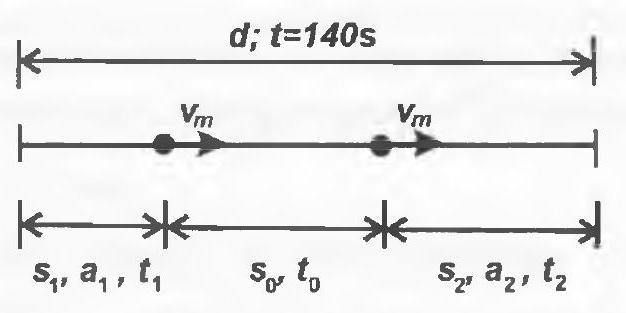
\includegraphics[max width=\textwidth, center]{2025_07_01_5b3ff9fa0d508c8e9f17g-236}

Fig. prob. 1.173\\
1.173. Deplasarea metroului între cele două staţii poate fi descompusă într-o mişcare cu viteză uniform accelerată, $a=1 \mathrm{~m} / \mathrm{s}^{2}$, urmată de 0 mişcare cu viteză constantă $v_{m}$ şi o mişcare frânată cu $a=-1 \mathrm{~m} / \mathrm{s}^{2}$, conform Fig. prob. 1.173, în care $s_{1}=s_{2}=s ;\left|a_{1}\right|=\left|a_{2}\right|=|a| ; t_{1}=t_{2}=t^{\prime}$.\\
Ecuațiile ce descriu mişcarea metroului sunt:

$$
s=\frac{a t^{\prime 2}}{2} ; v_{m}=a t^{\prime} ; s_{0}=v_{m} t_{0}
$$

iar condițiile impuse de problemă sunt:

$$
d=2 s+s_{0} ; t=2 t^{\prime}+t_{0}
$$

şi obținem un sistem de cinci ecuații cu cinci necunoscute: $s ; d ; t^{\prime} ; s_{0} ; t_{0}$. Eliminând necunoscutele $s ; t^{\prime} ; s_{0}$ şi $t_{0}$ obţinem:

$$
d=v_{m} t-\frac{v_{m}^{2}}{a}
$$

Înlocuind valorile numerice se determină $d=2750 \mathrm{~m}=2,75 \mathrm{~km}$.\\
1.174. $h_{\max }=\frac{v_{0}^{2}}{2 g}=\frac{100}{2 \cdot 10}=5 \mathrm{~m}$, deci piatra nu va atinge înălțimea $h=10 \mathrm{~m}$.\\
1.175. Considerăm mişcarea glontelui uniform frânată în scândură, iar ecuațiile ce descriu mişcarea sa sunt: $l=v_{0} t-\frac{a t^{2}}{2} ; 0=v_{0}-a t$ şi $0=v_{0}^{2}-2 a l$.\\
Din ultima relație putem afla accelerația de frânare în scândură:

$$
a=\frac{v_{0}^{2}}{2 l}=\frac{25 \cdot 10^{4}}{2 \cdot 5 \cdot 10^{-2}}=2,5 \cdot 10^{6} \mathrm{~m} / \mathrm{s}^{2}
$$

Dacă glontele întâlneşte scândura de grosime $d=2 \mathrm{~cm}$ atunci va avea o mişcare frânată cu accelerația $a=2,5 \cdot 10^{6} \mathrm{~m} / \mathrm{s}^{2}$, iar ecuațiile ce descriu mişcarea sa în scândură sunt: $d=v_{0} t-\frac{a t^{2}}{2} ; v=v_{0}-a t$ şi $v^{2}=v_{0}^{2}-2 a d$.

Din ultima relație putem afla viteza de ieşire din scândură a glontelui: $\quad v=\sqrt{v_{0}^{2}-2 a d}=100 \sqrt{15} \quad \mathrm{~m} / \mathrm{s}$. Impulsul primit de scândură este:

$$
p=m\left(v_{0}-v\right)=25 \cdot 10^{-3}(500-100 \sqrt{15})=2,8 \mathrm{~N}
$$

1.176. Mişcarea celor două corpuri este descrisă de Fig. prob. 1.176:

$$
\begin{array}{ll} 
& m_{2} a=m_{2} g-T \\
\text { şi } & m_{1} a=T-m_{1} g
\end{array}
$$

din care determinăm accelerația sistemului:

$$
a=\frac{m_{2}-m_{1}}{m_{1}+m_{2}} \cdot g
$$

\begin{center}
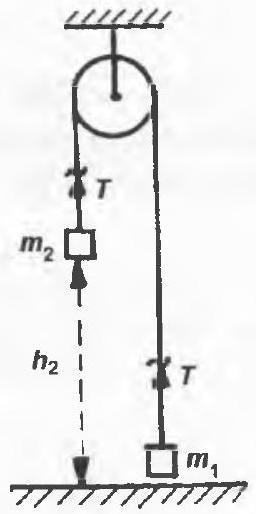
\includegraphics[max width=\textwidth]{2025_07_01_5b3ff9fa0d508c8e9f17g-237}
\end{center}

Fig. prob. 1.176

Mişcarea corpului $m_{1}$ pe distanța $h_{2}$ este dată de:

$$
h_{2}=\frac{a t^{2}}{2} ; v=a t \text { şi } v^{2}=2 a h_{2} .
$$

Din ultima relație determinăm:

$$
v=\sqrt{2 a h}=\sqrt{2 \cdot \frac{m_{2}-m_{1}}{m_{1}+m_{2}} \cdot g h_{2}}=\frac{2 \sqrt{15}}{3} \mathrm{~m} / \mathrm{s} .
$$

În continuare, corpul $m_{1}$ îşi continuă mişcarea pe verticală cu viteza inițială $v$, până la înălțimea maximă $h_{m}$ :

$$
h_{m}=\frac{v^{2}}{2 g}=\frac{4 \cdot 15}{9 \cdot 10}=\frac{2}{3} \mathrm{~m}
$$

Înălțimea atinsă de corp este:

$$
H=h_{2}+h_{m}=\frac{1}{2}+\frac{2}{3}=\frac{5}{6} \mathrm{~m}
$$

1.177. Spațiul parcurs la urcare în timpul $t_{u}$, cu viteza inițială $v_{0}$ şi accelerația de urcare $a_{u}=-g(\sin \alpha+\mu \cos \alpha)$ este egal cu spțiul parcurs la coborâre în timpul $t_{c}$, cu accelerația de coborâre $a_{c}=g(\sin \alpha-\mu \cos \alpha)$ :\\
sau

$$
S=v_{0} t_{u}-\frac{a_{u} t_{u}^{2}}{2}=\frac{a_{c} t_{c}^{2}}{2}
$$

sau $\quad g t_{u}^{2}(\sin \alpha+\mu \cos \alpha)-\frac{g(\sin \alpha+\mu \cos \alpha) t_{u}^{2}}{2}=\frac{g(\sin \alpha-\mu \cos \alpha)\left(3 t_{u}\right)^{2}}{2}$ sau $\mu=0,8$.

$$
\text { Înălțimea la care urcă corpul este } h=S \sin \alpha=\frac{v_{0}^{2}}{2 a_{u}} \sin \alpha=1 \mathrm{~m} \text {. }
$$

1.178. Corpul va merge pe traiectoria circulară până când forța centrifugǎ şi greutatea corpului au rezultantă nulă şi ținem cont că energia totală este constantă (Fig. prob. 1.178):\\
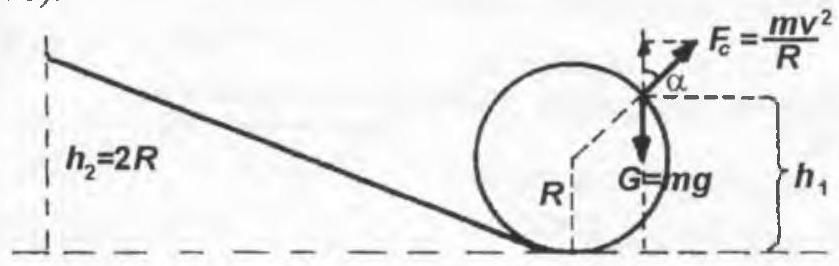
\includegraphics[max width=\textwidth, center]{2025_07_01_5b3ff9fa0d508c8e9f17g-238}

Fig. prob. 1.178

$$
G=F_{c} \cos \alpha \Rightarrow m g=\frac{m v^{2} \cos \alpha}{R} \Rightarrow v=\sqrt{g R \cos \alpha} ; \cos \alpha=\frac{2}{3}
$$

dar

$$
m g h=\frac{m v^{2}}{2}+m g R(1+\cos \alpha) \text { sau } 2 m g R=\frac{m g R \cos \alpha}{2}+m g h_{1} \Rightarrow h_{1}=1,67 \mathrm{~m} .
$$

1.179. $m g h+\frac{m v_{0}^{2}}{2}=\frac{m v^{2}}{2} \Rightarrow v=40 \mathrm{~m} / \mathrm{s}$.\\
1.180. $t_{1}=1 \mathrm{~s} ; t_{2}=2 \mathrm{~s}$ (Fig. prob. 1.180).

$$
s=v_{0} t_{1}-\frac{a t_{1}^{2}}{2} \quad \frac{v_{0}}{a}=t_{1}+\frac{t_{2}-t_{1}}{2}=\frac{t_{1}+t_{2}}{2} \Rightarrow v_{0}=0,45 \mathrm{~m} / \mathrm{s}
$$

\begin{center}
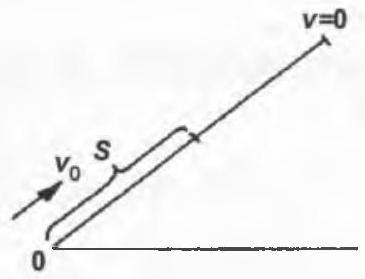
\includegraphics[max width=\textwidth]{2025_07_01_5b3ff9fa0d508c8e9f17g-239}
\end{center}

Fig. prob. 1.180\\
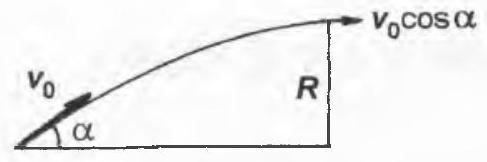
\includegraphics[max width=\textwidth, center]{2025_07_01_5b3ff9fa0d508c8e9f17g-239(1)}

Fig. prob. 1.181\\
1.181. (Fig. prob. 1.181)

$$
\frac{m v_{0}^{2} \cos ^{2} \alpha}{R}=m g \Rightarrow R=\frac{v_{0}^{2} \cos ^{2} \alpha}{g}=10 \mathrm{~m}
$$

1.182. $P=F \cdot v=2 m g \sin \alpha \cdot v=15000 \mathrm{~W}$.\\
1.183. $t_{u}=\frac{v_{0} \sin \alpha}{g} \quad t=2 t_{u} \quad s=t v_{0} \cos \alpha \quad W=\frac{m v_{0}^{2}}{2}=5 \mathrm{~J}$.\\
1.184. (Fig. prob. 1.184)

$$
\frac{m \omega^{2} R}{m g}=\frac{R}{1,5} \quad v=\frac{1}{2 \pi} \sqrt{\frac{g}{1,5}}=0,41 \mathrm{~s} .
$$

1.185. Din legea a $\amalg$-a a dinamicii:\\
$m=\frac{F_{1}}{a_{1}}=\frac{9}{3}=3 \mathrm{~kg} ; a_{2}=\frac{F_{2}}{m}=\frac{6}{3}=2 \mathrm{~m} / \mathrm{s}^{2}$\\
1.186. Din teorema variației impulsului:

$$
F=m \frac{\Delta v}{\Delta t}=0,2 \cdot \frac{15}{10^{-2}}=300 \mathrm{~N}
$$

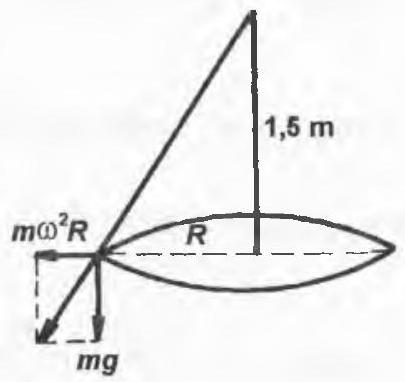
\includegraphics[max width=\textwidth, center]{2025_07_01_5b3ff9fa0d508c8e9f17g-239(2)}\\
1.187. Legea a doua a dinamicii se scrie: $m a=F_{t}-F_{f}$, deci\\
1.188. Din legea spațiului în mişcarea rectilinie uniform variată $l=\frac{a t^{2}}{2}$ rezultă $a=\frac{2 l}{t^{2}}$, încât $v=a t=\frac{2 l}{t^{2}} \cdot t=\frac{2 l}{t}=\frac{100}{10}=10 \mathrm{~m} / \mathrm{s}$.\\
1.189. Din legea vitezei în mişcarea rectilinie uniform variată $0=v_{0}-g \frac{\tau}{2}$, din care $v_{0}=10 \cdot \frac{10}{2}=50 \mathrm{~m} / \mathrm{s}$.\\
1.190. Forţa rezultantă va fi: $F=m g-\frac{m v^{2}}{R}=10^{3} \cdot 10-\frac{10^{3} \cdot 10^{2}}{10^{2}}=9 \mathrm{kN}$.\\
1.191. Se ştie că: $|F|=k x ; E_{p}=k \frac{x^{2}}{2}$, încât:

$$
E_{p}=k \frac{x^{2}}{2}=\frac{F}{x} \cdot \frac{x^{2}}{2}=F \frac{x}{2}=25 \cdot \frac{4 \cdot 10^{-2}}{2}=0,5 \mathrm{~J} .
$$

1.192. Din teorema conservării impulsului, $m_{1} \vec{v}_{1}+m_{2} \vec{v}_{2}=0$, încât

$$
p_{2}=\left|m_{2} \vec{v}_{2}\right|=\left|m_{1} \vec{v}_{1}\right|=0,5 \cdot 10=5 \mathrm{~N} \cdot \mathrm{~s}
$$

1.193. Se ştie că: $E_{c}=\frac{p^{2}}{2 m}$, încât $m=\frac{p^{2}}{2 E_{c}}=\frac{100}{20}=5 \mathrm{~kg}$.\\
1.194. $a_{1}=g \sin \alpha ; \quad s_{1}=\frac{h}{\sin \alpha}=\frac{1}{2} g \sin \alpha t_{1}^{2} \Rightarrow t_{1}=\frac{1}{\sin \alpha} \sqrt{\frac{2 h}{g}}=2 \mathrm{~s}$;\\
$F_{f}=m a_{2} ; F_{f}=\mu m g ; a_{2}=\mu g=2 \mathrm{~m} / \mathrm{s}^{2} ; E_{i}=E_{f} \Rightarrow E_{p f}=E_{c} \Rightarrow m g h=\frac{m v^{2}}{2}$\\
$\Rightarrow v=\sqrt{2 g h}=10 \mathrm{~m} / \mathrm{s} ; 0=v-\mu g t_{2} ; t_{2}=\frac{v}{\mu g}=5 \mathrm{~s} ; t=t_{1}+t_{2}=7 \mathrm{~s}$.\\
1.195. $a_{u}=\left(-G_{t}-F_{f}\right) / m=-g(\sin \alpha+\mu \cos \alpha) ; 0=\sqrt{v_{0}^{2}-2\left|a_{u}\right| l}$;

$$
\begin{aligned}
& l=\frac{v_{0}^{2}}{2\left|a_{u}\right|} ; \quad a_{c}=\frac{G_{t}-F_{f}}{m}=g(\sin \alpha-\mu \cos \alpha) ; 1=a_{c} t_{c}^{2} / 2 ; \\
& t_{c}=\sqrt{\frac{2 l}{a_{c}}}=\sqrt{\frac{2}{a_{c}} \cdot \frac{v_{0}^{2}}{2\left|a_{u}\right|}} ; \quad t_{u}=\frac{v_{0}}{\left|a_{u}\right|} ; \\
& \frac{t_{c}}{t_{u}}=\sqrt{\frac{\left|a_{u}\right|}{a_{c}}}=\sqrt{\frac{g(\sin \alpha+\mu \cos \alpha)}{g(\sin \alpha-\mu \cos \alpha)}}=\sqrt{\frac{1+\mu \operatorname{ctg} \alpha}{1-\mu \operatorname{ctg} \alpha}}=1,22 .
\end{aligned}
$$

1.196. $h=\frac{g t_{c}^{2}}{2} \Rightarrow t_{c}=\sqrt{\frac{2 h}{g}}=\sqrt{\frac{2 \cdot 400}{9,8}}=10 \mathrm{~s}$

$$
\Delta h=h-\frac{g\left(t_{c}-1\right)^{2}}{2}=490-\frac{9,8 \cdot 81}{2}=93,1 \mathrm{~m}
$$

1.197. $\quad v=\sqrt{v_{0}^{2}+2 a S} ; \quad a=\frac{v^{2}}{2 S}=\frac{900}{2 \cdot 500}=0,9 \mathrm{~m} / \mathrm{s}^{2} ; \quad F_{s}-F_{f}=m a$; $F_{s}=F_{f}+m a=1100 \mathrm{~N}$.\\
1.198. $L=\vec{F} \cdot \vec{d}=F \cdot d \cdot \cos \alpha, \vec{F}_{c p} \perp \vec{R} \Rightarrow \cos \alpha=0 \Rightarrow L=0$.\\
1.199. $\frac{m v^{2}}{L}=2 m g(\cos \beta-\cos \alpha) ; \quad T=F_{c f}+m g \cos \beta=\frac{m v^{2}}{L}+m g \cos \beta ;$ $T=m g(3 \cos \beta-2 \cos \alpha)=31,9 \mathrm{~N}$.\\
1.200. $F_{1}=G_{t}+F_{f}=m g(\sin \alpha+\mu \cos \alpha)$

$$
\begin{aligned}
& F_{2}=G_{t}-F_{f}=m g(\sin \alpha-\mu \cos \alpha) \\
& \frac{F_{1}}{F_{2}}=\frac{\sin \alpha+\mu \cos \alpha}{\sin \alpha-\mu \cos \alpha} \Rightarrow \mu=\frac{F_{1}-F_{2}}{F_{1}+F_{2}} \cdot \operatorname{tg} \alpha=1 / 3
\end{aligned}
$$

1.201. $L=\frac{1}{2} k A^{2}, F=k A \Rightarrow L=\frac{1}{2} F A \Rightarrow A=\frac{2 L}{F}=0,4 \mathrm{~m}$.\\
1.202. $\left.\begin{aligned} x & =x_{0}+v_{0} t+a \frac{t^{2}}{2} \\ x & =2+6 t-t^{2}\end{aligned} \right\rvert\, \Rightarrow x=2 \mathrm{~m} ; v_{0}=6 \mathrm{~m} / \mathrm{s} ; a=-2 \mathrm{~m} / \mathrm{s}^{2}$ (mişcarea uniform încetinită)

$$
\begin{aligned}
& v=v_{0}+a t \\
& \frac{v_{0}}{3}=v_{0}-2 t \Rightarrow t=\frac{v_{0}}{3}=\frac{6}{3}=2 \mathrm{~s}
\end{aligned}
$$

1.203. În prima jumătate $\frac{s}{2}=v_{0} t_{1}+\frac{a t_{1}^{2}}{2}$, viteza după prima jumătate $v=v_{0}+a t_{1}$, în a doua jumătate $\frac{s}{2}=v t_{2}+\frac{a t_{2}^{2}}{2}$.\\
$48=v_{0} \cdot 8+\frac{a}{2} \cdot 64$\\
$6=v_{0}+4 a$\\
$v=v_{0}+8 a$\\
$6=v_{0}+4 a$\\
$12=v_{0}+10 a$

$$
\begin{aligned}
& 48=\left(v_{0}+8 a\right) \cdot 4+\frac{a}{2} \cdot 16 \\
& 12=v_{0}+10 a \\
& v=v_{0}+8 a
\end{aligned}
$$

1.204. $G=m g=4 \cdot 10=40 \mathrm{~m} / \mathrm{s}^{2}<F$ (Fig. prob. 1.204)

$$
m a=F-G \Rightarrow a=\frac{F-G}{m}=5 \mathrm{~m} / \mathrm{s}^{2}, \text { în sus. }
$$

\begin{center}
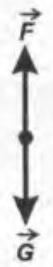
\includegraphics[max width=\textwidth]{2025_07_01_5b3ff9fa0d508c8e9f17g-242}
\end{center}

Fig. prob. 1.204\\
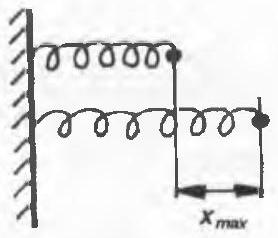
\includegraphics[max width=\textwidth, center]{2025_07_01_5b3ff9fa0d508c8e9f17g-242(1)}

Fig. prob. 1.205\\
1.205. (Fig. prob. 1.205)

$$
\frac{m v_{0}^{2}}{2}=\frac{K \cdot x_{\max }^{2}}{2} \Rightarrow x_{\max }=v_{0} \sqrt{\frac{m}{K}} .
$$

1.206. $\quad v_{1}=l_{1} \omega_{1}=l_{1} \frac{2 \pi}{T_{1}}$

$$
\begin{aligned}
& v_{2}=l_{2} \omega_{2}=l_{2} \frac{2 \pi}{T_{2}} \\
& \frac{v_{1}}{v_{2}}=\frac{1}{18} .
\end{aligned}
$$

1.207. Inițial $v_{0}=0 \quad p_{i}=0$\\
final $\left\{\begin{array}{l}v=v_{0}+g t \\ p_{f}=m v=1 \cdot 150=150 \mathrm{~kg} \cdot \mathrm{~m} / \mathrm{s}\end{array}\right.$

$$
G=m g \Rightarrow m=\frac{G}{g}=1 \mathrm{~kg}
$$

1.208. $H=\frac{g_{a} t^{2}}{2}$ spațiul parcurs în timpul $t$ de cădere. În timpul $t-1$ va parcurge o distanță $H^{\prime}=\frac{g_{a}(t-1)^{2}}{2}$. În ultima secundă parcurg distanța

$$
h=H-H^{\prime}=\frac{g_{a} t^{2}}{2}-\frac{g_{a}(t-1)^{2}}{2}=g_{a} t-\frac{g_{a}}{2} \Rightarrow t=\frac{2 h+g_{a}}{2 g_{a}} .
$$

După înlocuirea lui $t$ din ultima relație în prima expresie a lui $H$ obținem:

$$
H=\frac{g_{a}}{2} \frac{\left(2 h+g_{a}\right)^{2}}{4 g_{a}}=\frac{\left(2 h+g_{a}\right)^{2}}{8 g_{a}}=\frac{8^{2}}{8 \cdot 4}=4 \mathrm{~m} .
$$

1.209. Din Fig. prob. 1.209 în care $S$ reprezintă poziția de echilibru a sferei în timpul mişcării accelerate a cilindrului rezultă:

$$
\operatorname{tg} \theta=\frac{m a}{m g}=\frac{a}{g}=\frac{g}{g}=1 \Rightarrow \theta=45^{\circ} .
$$

\begin{center}
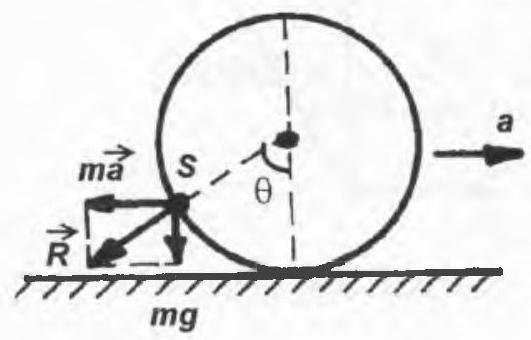
\includegraphics[max width=\textwidth]{2025_07_01_5b3ff9fa0d508c8e9f17g-243}
\end{center}

Fig. prob. 1.209\\
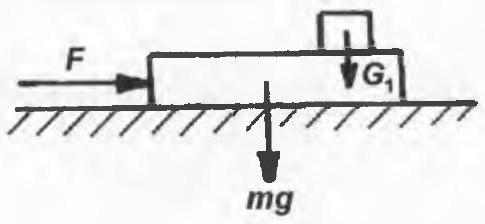
\includegraphics[max width=\textwidth, center]{2025_07_01_5b3ff9fa0d508c8e9f17g-243(1)}

Fig. prob. 1.210\\
1.210. Legea de mişcare a scândurii este (Fig. prob. 1.210):


\begin{equation*}
m a=F-F_{f_{1}}-F_{f_{2}} \tag{1}
\end{equation*}


unde $F_{f_{1}}=\frac{G_{1}}{g} \cdot a=\mu_{1} G_{1}$,\\
$\operatorname{iar} \quad F_{f_{2}}=\left(m g+G_{1}\right) \cdot \mu_{2}$.\\
Din egalitatea (2) rezultă


\begin{equation*}
a=\mu_{1} g . \tag{4}
\end{equation*}


Introducem (2), (3) şi (4) în ecuația (1) şi obținem:\\
sau

$$
m \mu_{1} g=F-G_{1} \cdot \mu_{1}-\left(m g+G_{1}\right) \cdot \mu_{2}
$$


\begin{equation*}
F=m \mu_{1} g+G_{1} \cdot \mu_{1}+\left(m g+G_{1}\right) \cdot \mu_{2} \tag{5}
\end{equation*}


Numeric din (5) obținem: $\quad F=22,5 \mathrm{~N}$.\\
1.211. Din Fig. prob. 1.211 rezultă că:


\begin{equation*}
\vec{F}_{f}+\vec{G}+\vec{F}+\vec{N}=0 \tag{1}
\end{equation*}


în cazul mișcării cu viteză constantă. Forța de frecare are mărimea:


\begin{equation*}
F_{f}=\mu(G+F \cos \theta) . \tag{2}
\end{equation*}


\begin{center}
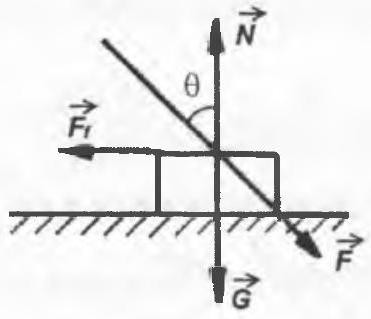
\includegraphics[max width=\textwidth]{2025_07_01_5b3ff9fa0d508c8e9f17g-244}
\end{center}

Fig. prob. 1.211\\
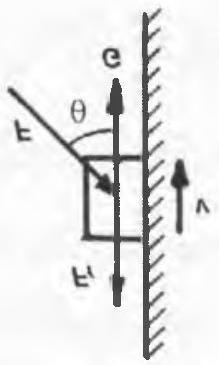
\includegraphics[max width=\textwidth, center]{2025_07_01_5b3ff9fa0d508c8e9f17g-244(1)}

Fig. prob, 1.212

Proiecția relației (1) pe direcția orizontală este:


\begin{equation*}
F \sin \theta=\mu \cdot F_{f} . \tag{3}
\end{equation*}


Din (2) şi (3) rezultă:

$$
F=\frac{\mu \cdot G}{\sin \theta-\mu \cos \theta}=\frac{0,1 \cdot 5 \cdot 10}{\sin 30^{\circ}-0,1 \cos 30^{\circ}}=12,09 \mathrm{~N} .
$$

1.212. Din Fig. prob. 1.212 rezultă:


\begin{equation*}
F \cos \theta+F_{f}=G . \tag{1}
\end{equation*}


Din definiția forței de frecare


\begin{equation*}
F_{f}=\mu \cdot F_{n}=\mu \cdot F \sin \theta . \tag{2}
\end{equation*}


Din relațiile (1) şi (2) rezultă:

$$
F=\frac{m g}{\cos \theta+\mu \sin \theta}=\frac{5 \cdot 10}{\frac{\sqrt{2}}{2}+0,3 \cdot \frac{\sqrt{2}}{2}}=176,25 \mathrm{~N} .
$$

1.213. Variația de greutate $\Delta G=G_{p}-G_{e}$, unde $G_{p}=m g$ $G_{e}=m g-m \omega^{2} R$. Deci

$$
\Delta G=m \omega^{2} R=m \frac{4 \pi^{2}}{T^{2}} R=100 \frac{4 \pi^{2}}{(24)^{2}(3600)^{2}}=64 \cdot 10^{5} \mathrm{~N}=3,37 \mathrm{~N} .
$$

1.214. $F_{1}=7 x_{1}+3, \quad F_{2}=7 x_{2}+3$

$$
\begin{aligned}
& F_{m}=\frac{F_{1}+F_{2}}{2}=\frac{7\left(x_{1}+x_{2}\right)+6}{2} \\
& L=F_{m} d=F_{m}\left(x_{2}-x_{1}\right)=\frac{7\left(x_{1}+x_{2}\right)+6}{2}\left(x_{2}-x_{1}\right) \\
& L=\frac{7 \cdot 8+6}{2} \cdot 2=62 \mathrm{~J}
\end{aligned}
$$

1.215. Vezi Fig. prob. 1.215.

$$
\begin{aligned}
& \bar{v}_{2}=\bar{v}_{1}+\bar{v}_{v a n t} ; \quad V_{1}=234 \mathrm{~km} / \mathrm{h}=65 \mathrm{~m} / \mathrm{s} \\
& v_{2}=\sqrt{65^{2}-25^{2}}=60 \mathrm{~m} / \mathrm{s} \\
& v_{2}=216 \mathrm{~km} / \mathrm{h}
\end{aligned}
$$

$$
\alpha=\operatorname{arctg} \frac{v_{v a n t}}{v_{2}}=\operatorname{arctg} \frac{25}{60}=\operatorname{arctg} \frac{5}{12} .
$$

\begin{center}
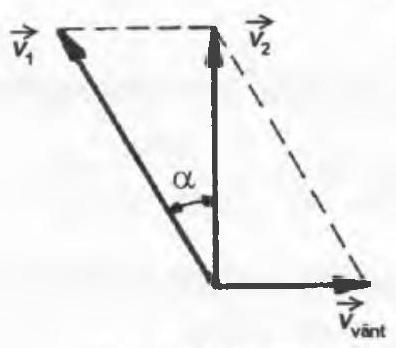
\includegraphics[max width=\textwidth]{2025_07_01_5b3ff9fa0d508c8e9f17g-245}
\end{center}

Fig. prob. 1.215\\
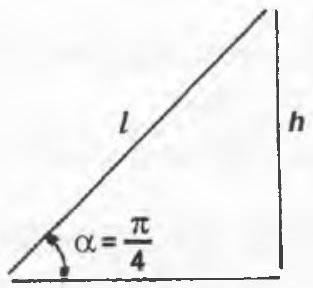
\includegraphics[max width=\textwidth, center]{2025_07_01_5b3ff9fa0d508c8e9f17g-245(1)}

Fig. prob. 1.216\\
1.216. Vezi Fig. prob. $1.216 ; l=\frac{h}{\sin \alpha}=\frac{4,4}{\sqrt{2} / 2}=4,4 \sqrt{2} \mathrm{~m}$\\
$l=v_{0} t-\frac{1}{2} a t^{2}$\\
$a=g(\sin \alpha+\mu \cos \alpha)=10\left(\frac{\sqrt{2}}{2}+0,1 \frac{\sqrt{2}}{2}\right)=5,5 \sqrt{2} \mathrm{~m} / \mathrm{s}^{2}$\\
$t^{2}-\frac{2 v_{0}}{a} t+\frac{2 l}{a}=0$\\
$t=\frac{v_{0}}{a} \pm \sqrt{\frac{v_{0}^{2}}{a}-\frac{2 l}{a}}=\frac{11}{5,5 \sqrt{2}} \pm \sqrt{\left(\frac{11}{5,5 \sqrt{2}}\right)^{2}-\frac{2 \cdot 4,4 \sqrt{2}}{5,5 \sqrt{2}}}=$\\
$=\sqrt{2} \pm \sqrt{(\sqrt{2})^{2}-1,6}=\sqrt{2} \pm \sqrt{0,4}$\\
$t=1,414 \pm 0,633=\left\{\begin{array}{l}2,037 \cong 2 \mathrm{~s} \\ 0,781 \cong 0,78 \mathrm{~s}\end{array}\right.$\\
Convine soluția mai mică: $t=0,78 \mathrm{~s}$.\\
1.217. Conform legii conservării energiei:

$$
m_{2} g h=\frac{\left(m_{1}+m_{2}\right) v^{2}}{2} \Rightarrow v=\sqrt{\frac{2 m_{2} g h}{m_{1}+m_{2}}} .
$$

1.218. Constanta elastică a resortului este: $K=\frac{G}{\Delta l}=\frac{m g}{\Delta l}$. În cazul mişcării pe cerc, forța ce acționează asupra resortului este: $F=\sqrt{\left(\frac{m v^{2}}{R}\right)^{2}+(m g)^{2}}$.

Deci: $\Delta l^{\prime}=\frac{F}{\frac{m g}{\Delta l}}=\Delta l \frac{\sqrt{\frac{v^{4}}{R^{2}}+g^{2}}}{g}$.\\
1.219. În cazul când $m$ alunecă pe suprafața lui $M$, accelerațiile față de sol vor fì: $a_{1}=\frac{F-\mu m g}{M}, a_{2}=\mu g$. Deci: $a=a_{1}-a_{2}=\frac{F-\mu m g}{M}-\mu g$.\\
1.220. Forța care acționează asupra corpului în lungul planului este:\\
$F=m g \sin \alpha+m a \cos \alpha-\mu(m g \cos \alpha-m a \sin \alpha)$.\\
Deci: $a=g \sin \alpha+a \cos \alpha-\mu(g \cos \alpha-a \sin \alpha)$.\\
1.221. $F=m \frac{v}{t}+\mu m g, \operatorname{deci} t=\frac{m v}{F-\mu m g}$.\\
1.222. $h=\frac{g t^{2}}{2} ; \quad h-h^{\prime}=\frac{g(t-\tau)^{2}}{2}$. Deci $\frac{g t^{2}}{2}=h^{\prime}+\frac{g(t-\tau)^{2}}{2}$, unde $h^{\prime}=k h=k \frac{g t^{2}}{2}$. Rezultă: $t=\tau \cdot \frac{1+\sqrt{1-k}}{k}$.\\
1.223. Conform Fig. prob. 1.223 , acceleraţia $a=\frac{F \cos \alpha-\mu(m g-F \sin \alpha)}{m}$.\\
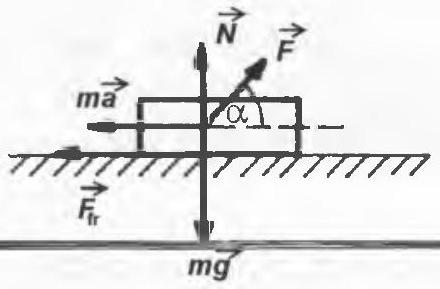
\includegraphics[max width=\textwidth, center]{2025_07_01_5b3ff9fa0d508c8e9f17g-246}

Fig. prob. 1.223

În repaus, $a \leq 0$, astfel că :

$$
F \leq \frac{\mu m g}{\cos \alpha+\mu \sin \alpha}
$$

$\mu m g$\\
1.224. Ecuațiile de mişcare ale celor două bile se scriu: $y_{1}=v_{01} t-\frac{1}{2} g t^{2}$ şi $y_{2}=v_{01}(t-\tau)-\frac{1}{2} g(t-\tau)^{2}$. Din condiția de întâlnire, $y_{1}=y_{2}$, adică

$$
v_{01} t-\frac{1}{2} g t^{2}=v_{02}(t-\tau)-\frac{1}{2} g(t-\tau)^{2}, \Rightarrow t=\frac{v_{02} \tau+\frac{1}{2} g \tau^{2}}{v_{02}-v_{01}+g \tau}=2 \mathrm{~s}
$$

Timpii de urcare şi coborâre ai primei bile sunt $t_{u}=t_{c}=\frac{v_{01}}{g}=1 \mathrm{~s}$, deci $\tau=t_{u}+t_{c}$, adică întâlnirea bilelor are loc pe sol în momentul pornirii celei de a doua bile şi nu depinde de viteza inițială a celei de a doua bile.\\
1.225. Din formula lui Galilei, $0=v_{0}^{2}-2 a d$, rezultă accelerația de frânare, $a=\frac{v_{0}^{2}}{2 d}$ şi forța de frânare $F=m a=\frac{v_{0}^{2}}{2 d}=5 \cdot 10^{5} \mathrm{~N}$.\\
1.226. Conform legii de mişcare pe planul înclinat, la coborâre, $s=\frac{1}{2} a t^{2}=\frac{1}{2} g(\sin \alpha-\mu \cos \alpha)=b t^{2}$, de unde $\mu=\operatorname{tg} \alpha-\frac{2 b}{g \cos \alpha}=0,30$.\\
1.227. Inițial, resortul este alungit cu $x_{0}=\frac{m_{2} g}{k}$, iar după deblocare, cu $x_{1}=\frac{T}{k}=\frac{2 m_{1} m_{2} g}{k\left(m_{1}+m_{2}\right)}$. Alungirea suplimentară este

$$
x_{1}-x_{0}=\frac{m_{2} g}{k} \cdot \frac{m_{1}-m_{2}}{m_{1}+m_{2}}=0,024 \mathrm{~m}
$$

1.228. Conform Fig. prob. 1.228,

$$
F=\mu m_{1} g+k x, \quad \mu m_{2} g=k x
$$

de unde $F=\mu\left(m_{1}+m_{2}\right) g$.\\
1.229. Puterea, $P=\bar{F} \cdot \bar{v}=m(a+\mu g) \frac{v}{2}$ şi puterea la viteză maximă, $P=\mu m g v$, de\\
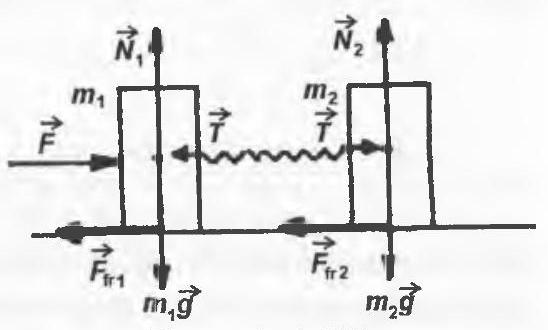
\includegraphics[max width=\textwidth, center]{2025_07_01_5b3ff9fa0d508c8e9f17g-247}

Fig. prob. 1.228 unde $a=\mu g=0,15 \mathrm{~m} / \mathrm{s}^{2}$.\\
1.230. Din conservarea energiei, $\frac{m v^{2}}{2}=\frac{k x^{2}}{2}$, rezultă $v=x \sqrt{\frac{k}{m}}$ şi distanța parcursă pe orizontală este: $d=v t=x \sqrt{\frac{k}{m}} \sqrt{\frac{2 h}{g}}=4 \mathrm{~m}$.\\
1.231. Randamentul este o mărime adimensionalã.\\
1.232. Răspuns corect: B).\\
1.233. Biciclistul merge $t_{1}=\frac{72 \mathrm{~km}}{18 \mathrm{~km} / \mathrm{h}}=4 \mathrm{~h}$ ca şi motociclistul. În aceste 4 h , motociclistul parcurge $D+72 \mathrm{~km}=4 \cdot 72 \mathrm{~km}$, deci $D=216 \mathrm{~km}$.\\
1.234. $v_{m}=\frac{v_{0}+v_{\text {final }}}{2}=\frac{g \cdot t}{2}=\frac{9,8 \cdot 3}{2}=14,7 \mathrm{~m} / \mathrm{s}$.\\
1.235. $s_{1}=\frac{v_{1}^{2}}{2 a}, \quad s_{2}=\frac{v_{2}^{2}}{2 a} \Rightarrow s_{2}=\left(\frac{v_{2}}{v_{1}}\right)^{2} \cdot s_{1}=\left(\frac{108}{18}\right)^{2} \cdot 3=108 \mathrm{~m}$.\\
1.236. Timpul de cădere rezultat din ecuația:

$$
h=v_{0 y} t_{c}+\frac{g t_{c}^{2}}{2}
$$

unde $v_{0 y}=v_{0} \sin \alpha$. Se obține $t_{c}=2 \mathrm{~s}$. Viteza pe sol este:

$$
\begin{aligned}
v & =\sqrt{v_{0 x}^{2}+v_{0 y}^{2}}=\sqrt{v_{0}^{2} \cos ^{2} \alpha+\left(v_{0 y}+g t_{c}\right)^{2}}= \\
& =\sqrt{40^{2} \cdot \frac{3}{4}+(20+10 \cdot 2)^{2}}=20 \sqrt{7} \cong 52,9 \mathrm{~m} / \mathrm{s}
\end{aligned}
$$

1.237. Lucrul mecanic este nul, corpul nu se mişcă.\\
1.238. $E_{c 1}=\frac{m v^{2}}{2}, \quad E_{c 2}=\frac{\frac{m}{2}(2 v)^{2}}{2}=m v^{2}=2 E_{c 1}$.\\
1.239. Răspuns corect: A).\\
1.240. D) este afirmația falsă, deoarece forța centripetă acționează într-adevăr asupra punctului material şi-i determină mişcarea circulară, dar forța centrifugă nu acționează asupra lui, ci asupra mediului, fiind reacțiunea forței centripete. Dacă, prin absurd, aceste două forțe ar acționa asupra punctului material, atunci s-ar anula reciproc, iar mişcarea corpului ar fi rectilinie şi uniformă, conform principiului inerției.\\
1.241. Afirmația falsă este C ), forța centrifugă nu acționează asupra corpului, ci asupra mediului, fiind reacțiunea la forța centripetă. Forța centripetă este cea care acționează asupra punctului material şi-l determină să se mişte pe traiectorie circulară.\\
1.242. Asupra punctului material acționează simultan forța centripetă şi pseudoforța centrifugă de inerție, a căror rezultantă este nulă, iar corpul apare ca fiind în repaus față de sistemul de referință neinerțial solidar cu corpul. Afirmația falsă este D ), deoarece forța centrifugă are puncte de aplicație diferite: este creată de punctul material şi acționează asupra mediului, iar forța centripetă este creată de mediu şi acționează asupra punctului material.\\
1.243. Afirmația adevărată este A ).\\
1.244. Să presupunem că masa corpului este $m$ şi că se mişcă spre perete cu viteza $v$. Forţa medie la ciocnirea elastică este $F_{\text {elastic }}=\frac{\Delta p_{\text {elastic }}}{\Delta t}=\frac{2 m v}{\Delta t}$. Forţa medie la ciocnirea plastică este $F_{\text {plastic }}=\frac{\Delta p_{\text {plastic }}}{\Delta t}=\frac{m v}{\Delta t}$. Raportul corect este $\frac{F_{\text {elastic }}}{F_{\text {plastic }}}=2$.\\
1.245. Folosind conservarea impulsului, obținem că deplasarea bărcii este dată de relaţia $d=\frac{m}{m+M} l$ care nu depinde de timp.\\
1.246. Notăm vitezele celor două bile $\mathrm{cu} \vec{v}_{1}$, respectiv $\vec{v}_{2}$, iar masele lor cu $m_{1}=m_{2}=m$. Folosind conservarea impulsului şi conservarea energiei totale (mecanică plus căldură) obținem relația pentru cantitatea de căldură degajată în urma ciocnirii sub forma $Q=\frac{1}{4} m\left(v_{1}+v_{2}\right)^{2}$. Dacă cele două viteze sunt egale în modul, rezultă $Q=m v^{2}$. Dacă una dintre viteze se triplează, avem $Q^{\prime}=\frac{1}{4} m(v+3 v)^{2}=4 m v^{2}$.\\
1.247. În primul caz, energia potențială elastică este $E=\frac{1}{2} k(\Delta l)^{2}$, unde $k$ este constanta elastică a resortului, iar $\Delta l$ comprimarea acestuia. Aceasta se transformă succesiv în energie cinetică a corpului, apoi în energie potențială gravitațională; înălțimea maximă este $h=\frac{1}{2 m g} k(\Delta l)^{2}$. În lipsa frecărilor, câmpul gravitațional\\
este un câmp conservativ de forțe, înălțimea maximă în cel de-al doilea caz fiind $h^{\prime}=\frac{1}{2 m g} k\left(\frac{1}{2} \Delta l\right)^{2}=\frac{1}{4} h$.\\
1.248. Ca o consecință a conservării energiei și impulsului, prima bilă se opreşte după ciocnire; răspunsul corect este $F$ ).\\
1.249. În punctul B (Fig. prob. 1.249), particula are viteza $v$ şi se desprinde dacă $F_{c}=G \cos \theta$, adică $\frac{m v^{2}}{R}=m g \cos \theta \Rightarrow v=\sqrt{R g \cos \theta}$

Aplicând legea conservării energiei, se obține: $E_{\text {tot }}^{\mathrm{A}}=E_{\text {tot }}^{\mathrm{B}} \Rightarrow$\\
$m g 2 R=m g(R+R \cos \theta)+\frac{m v^{2}}{2} \Rightarrow v=\sqrt{2 R g(1-\cos \theta)}$\\
(2)

Egalând (1) şi (2) se obține pentru unghiul sub care particula se desprinde $\cos \theta=\frac{2}{3}$.\\
\includegraphics[max width=\textwidth, center]{2025_07_01_5b3ff9fa0d508c8e9f17g-250(1)}

Fig. prob. 1.249\\
\includegraphics[max width=\textwidth, center]{2025_07_01_5b3ff9fa0d508c8e9f17g-250}

Fig. prob. 1.250\\
1.250. În punctul B (Fig. prob. 1.250) particula se desprinde și cade oblic, cu viteza inițială $v$ de componente $v_{0 x}=v \cos \theta, v_{0 y}=v \sin \theta$. În punctul B: $\frac{m v^{2}}{R}=m g \cos \theta \Rightarrow v=\sqrt{R g \cos \theta} \Rightarrow v=\sqrt{\frac{2}{3} R g}$.\\
Când atinge pământul componentele vitezei vor fi: $v_{x}=v_{0 x}=v \cos \theta$,


\begin{equation*}
v_{y}=v_{0 y}+g t \Rightarrow t=\frac{v_{y}-v_{0 y}}{g} \tag{1}
\end{equation*}


Din ecuația Galilei: $v_{y}=\sqrt{v^{2} \sin ^{2} \theta+2 \operatorname{Rg}(1+\cos \theta)} \mathrm{cu}$

\[
\left\{\begin{array}{l}
\cos \theta=\frac{2}{3} \Rightarrow v_{y}=\frac{10}{3} \sqrt{\frac{R g}{3}}  \tag{2}\\
v=\sqrt{\frac{2}{3} R g}
\end{array}\right.
\]

Timpul cât durează cǎderea va fi, folosind (1) şi (2): $t=\frac{1}{3} \sqrt{\frac{10 R}{3 g}}(\sqrt{10}-1)$ şi $\mathrm{A}^{\prime} \mathrm{M}=\frac{13 \sqrt{5}}{27} R$.\\
1.251. Pentru o porțiune de lungime $A B$ (Fig. prob. 1.251) şi masă $\Delta m$, rezultanta tensiunilor $\vec{T}_{1}$ şi $\vec{T}_{2}$ care se exercită în punctele $A$, respectiv $B$, are mărimea:

$$
R_{T_{\mathrm{AB}}}=2 T \cos \left(\frac{\pi}{2}-\Delta \theta\right)=2 T_{\mathrm{AB}} \sin (\Delta \theta),
$$

unde $2 \Delta \theta$ este unghiul la centru sub care se vede arcul $\hat{A B}$. La echilibru, această rezultantă este egală cu forța centripetă $R_{T_{\mathrm{AB}}}=\frac{\Delta m v^{2}}{r} \Rightarrow$\\
$\Rightarrow 2 T_{\hat{\mathrm{AB}}} \sin (\Delta \theta)=\frac{\Delta m \cdot v^{2}}{r} \Rightarrow T_{\hat{\mathrm{AB}}}=\frac{\Delta m \cdot v^{2}}{2 r \sin (\Delta \theta)}$.\\
\includegraphics[max width=\textwidth, center]{2025_07_01_5b3ff9fa0d508c8e9f17g-251}

Fig. prob. 1.251

Masa porțiunii considerate este $\Delta m=\rho S r \cdot 2 \Delta \theta$, unde $\rho=$ densitatea materialului, $S=$ secțiunea benzii.\\
1.252. Condiția ca maşina să nu cadă în $A$ (Fig. prob. 1.252) este:

$$
\frac{m v^{2}}{R}=m g \Rightarrow v=\sqrt{R g} .
$$

Dacă intră (în $B$ ) cu viteza $v_{0}$, atunci conform relației Galilei, va avea în $A$ viteza $v^{2}=v_{0}^{2}-2 g h$. Viteza de intrare va fi:\\
$v_{0}=\sqrt{v^{2}+2 g h}=\sqrt{R g+6 R g}=\sqrt{7 R g} \Rightarrow v_{0}=26,1 \mathrm{~m} / \mathrm{s}$.\\
1.253. Dacă maşinile pleacă $\operatorname{din} A$ în repaus, viteza în $B$ va fi:

$$
v^{2}=2 g h \Rightarrow v=\sqrt{2 g h} .
$$

În Fig. prob. 1.253, pasagerii suportă greutatea $G=m g$ şi forța centrifugă $F_{c}=\frac{m v^{2}}{R}$. Forța totală va fi $R=G+F_{c}=m \cdot 8 g \Rightarrow m g+\frac{m \cdot 2 g h}{R}=8 m g \Rightarrow$ $R=\frac{2}{7} h \Rightarrow R=14,3 \mathrm{~m}$.\\
\includegraphics[max width=\textwidth, center]{2025_07_01_5b3ff9fa0d508c8e9f17g-252(1)}

Fig. prob. 1.252\\
\includegraphics[max width=\textwidth, center]{2025_07_01_5b3ff9fa0d508c8e9f17g-252}

Fig. prob. 1.253\\
1.254. Ciocnirea proiectil - pendul este total inelastică. Din conservarea impulsului rezultă


\begin{equation*}
\left(m_{1}+m_{2}\right) v=m_{1} v_{1} \Rightarrow v=\frac{m_{1} v_{1}}{m_{1}+m_{2}} \tag{1}
\end{equation*}

După ciocnire, pendulul şi proiectilul se ridică la înălţimea $h$. Din conservarea energiei rezultă $\left(m_{1}+m_{2}\right) \frac{v^{2}}{2}=\left(m_{1}+m_{2}\right) g h \Rightarrow v=\sqrt{2 g h}$

Egalând (1) şi (2) rezultă: $\frac{m_{1} v_{1}}{m_{1}+m_{2}}=\sqrt{2 g h} \Rightarrow v_{1}=\frac{m_{1}+m_{2}}{m_{1}} \sqrt{2 g h}=798 \mathrm{~m} / \mathrm{s}$\\
1.255. În sistemul de axe indicat pe Fig. prob. 1.255 , ecuaţiile de mişcare ale corpului vor fi (se neglijează rezistența aerului): $x=v_{0} t ; y=h-\frac{1}{2} g t^{2}$. În punctul căderii $y=0 \rightarrow h=\frac{1}{2} g t_{\text {cădere }}^{2}$. Expresiile celor două componente ale vitezei vor fi:

$$
v_{x}=v_{0}, v_{y}=-g t ; \operatorname{tg} \alpha=\frac{v_{y}}{v_{x}} \operatorname{sau} \operatorname{tg} 60^{\circ}=\frac{g t_{\text {cădere }}}{v_{0}}
$$

Dar $\operatorname{tg} \alpha=\frac{\sin \alpha}{\cos \alpha} \Rightarrow \frac{\sqrt{3} / 2}{1 / 2}=\sqrt{3}$ şi rezultă: $\sqrt{3}=\frac{9,8 \frac{\mathrm{~m}}{\mathrm{~s}^{2}} t_{\text {cădere }}}{15 \mathrm{~ms}}$.\\
De aici: $h=\frac{1}{2} g t_{\text {cădere }}^{2}$ sau $h=\frac{1}{2} g\left(\frac{v_{0} \operatorname{tg} 60^{\circ}}{g}\right)^{2}=\frac{v_{0}^{2} \operatorname{tg}^{2} 60^{\circ}}{2 \mathrm{~g}}=34,4 \mathrm{~m}$.\\
\includegraphics[max width=\textwidth, center]{2025_07_01_5b3ff9fa0d508c8e9f17g-253(2)}

Fig. prob. 1.255\\
\includegraphics[max width=\textwidth, center]{2025_07_01_5b3ff9fa0d508c8e9f17g-253(1)}

Fig. prob. 1.256\\
1.256. $F_{\text {apäsare }}=\frac{4}{5} G=G-F_{c f}$ sau $\frac{1}{5} G=F_{c f} \Rightarrow \frac{1}{5} m g=\frac{m v^{2}}{R} \Rightarrow$

$$
v=72 \frac{\mathrm{~km}}{\mathrm{~h}}=20 \frac{\mathrm{~m}}{\mathrm{~s}} . \text { Rezultă: } R=\frac{5 v^{2}}{g}=200 \mathrm{~m}
$$

1.257. În momentul desprinderii (Fig. prob. 1.257):

$$
F_{c f}=G_{N} \Rightarrow \frac{m v^{2}}{R}=G \sin \alpha
$$

unde $\sin \alpha=\frac{h_{2}}{R}$. La conservarea energiei mecanice: $m g h_{1}=\frac{m v^{2}}{2} \Rightarrow v^{2}=2 g h_{1}$ şi

$$
\frac{m \cdot 2 g h_{1}}{R}=m g \frac{R-h_{1}}{R} \Rightarrow 2 h_{1}=R-h_{1} \Rightarrow h_{1}=\frac{R}{3}=1 \mathrm{~m} .
$$

\begin{center}
\includegraphics[max width=\textwidth]{2025_07_01_5b3ff9fa0d508c8e9f17g-253(3)}
\end{center}

Fig. prob. 1.257\\
\includegraphics[max width=\textwidth, center]{2025_07_01_5b3ff9fa0d508c8e9f17g-253}

Fig. prob. 1.258\\
1.258. Cum $v=$ const., rezultǎ $a=0$, deci $\sum F_{i}=m a=0$ şi de aici $F_{\text {frecare }}=F_{\text {orizontal }} \quad$ sau $\quad \mu F_{\text {apăsare }}=F \cos \alpha \quad \Rightarrow \quad \mu(m g-F \sin \alpha)=F_{\text {orizontal }}$ (Fig. prob. 1.258).

Deci $\mu=\frac{F_{\text {orizontal }}}{m_{\text {sanie }} \cdot g-F \sin \alpha} \approx 0,76$.\\
1.259. $v=15 \frac{\mathrm{~m}}{\mathrm{~s}}$;\\
$P=\frac{L}{t}=\frac{F d}{t}=F v=450 \mathrm{~kW}$.\\
1.260. $v=30 \mathrm{~m} / \mathrm{s} ; P=6 \cdot 10^{4} \mathrm{~W} ; P=\frac{L}{t}=\frac{F \cdot d}{t}=F \cdot v \rightarrow F=\frac{P}{v}$.

Dar: $P=\frac{L}{t}=\frac{\eta E}{t} \Rightarrow t=\frac{\eta E}{P}=\frac{V \frac{E s}{V}}{P}$. Spațiul străbătut va fi: $S=v t=4 \mathrm{~km}$.\\
1.261. $L=F \cdot d \Rightarrow d=\frac{L}{F}=100 \mathrm{~m}$

Dar: $d=\frac{a t^{2}}{2} \Rightarrow a=\frac{2 d}{t^{2}}=2 \frac{\mathrm{~m}}{\mathrm{~s}^{2}}$.\\
1.262. $\alpha=30^{\circ} ; m=1 \mathrm{~kg} ; \mu=\frac{F_{\text {frecare }}}{F_{\text {apăsare }}}=0,2 ; g=10 \mathrm{~m} / \mathrm{s}^{2}$.

De-a lungul planului înclinat (Fig. prob. 1.262) forțele trebuie să-şi facă echilibru, adică:\\
$G_{t}-F_{\text {frecare }}-F_{\text {proiectat }}=0$ sau:\\
$m g \sin \alpha-\mu m g \cos \alpha=F \cos \alpha$, de unde $F_{\text {min }}=m g(\operatorname{tg} \alpha-\mu)=3,77 \mathrm{~N}$.\\
\includegraphics[max width=\textwidth, center]{2025_07_01_5b3ff9fa0d508c8e9f17g-254(1)}

Fig. prob. 1.262\\
\includegraphics[max width=\textwidth, center]{2025_07_01_5b3ff9fa0d508c8e9f17g-254}

Fig. prob. 1.263\\
1.263. Vezi Fig. prob. 1.263.\\
$\operatorname{tg} \alpha=\frac{F_{c f}}{G}=\frac{m v^{2}}{R \cdot m g}=\frac{v^{2}}{R g}$ sau $v^{2}=\lg \frac{\sin ^{2} \alpha}{\cos \alpha}=\omega^{2} R^{2}=\omega^{2} l^{2} \sin ^{2} \alpha ;$\\
$\cos \alpha=\frac{g}{\omega^{2} l}=\frac{10 \mathrm{~m} / \mathrm{s}^{2} \cdot \mathrm{~s}^{2}}{49 \cdot 0,4 \mathrm{~m}}=\frac{25}{49} ; \sin ^{2} \alpha=1-\cos ^{2} \alpha=1-\frac{25^{2}}{49^{2}}$;

$$
E_{\text {cinetic }}=\frac{m v^{2}}{2}=\frac{m}{2} \lg \frac{\sin ^{2} \alpha}{\cos \alpha} \approx 5,8 \mathrm{~J}
$$

1.264. În lungul axei $\mathrm{O} x$ mișcarea este uniformă, cu viteza $v_{0 x}$.

$$
v_{0 x}=v_{0} \cos \alpha ; v_{0 y}=v_{0} \sin \alpha . \text { Dar } a_{x}=0 ; a_{y}=-g
$$

Rezultă: $v_{x}=v_{0} \cos \alpha ; v_{y}=v_{0} \sin \alpha-g t$.\\
$x=v_{0} t \cos \alpha ; y=y_{0}+v_{0} t \sin \alpha-\frac{g t^{2}}{2}$.\\
La noi, în condițiile problemei:\\
$h_{1}=y_{0}+v_{0} t_{1} \sin \alpha-\frac{g t_{1}^{2}}{2} ; h_{2}=y_{0}+v_{0} t_{2} \sin \alpha-\frac{g t_{2}^{2}}{2}$.\\
Pentru cazul $h_{1}=h_{2}$, obținem: $v\left(t_{2}-t_{1}\right) \sin \alpha-\frac{g}{2}\left(t_{2}^{2}-t_{1}^{2}\right)=0$.\\
$\alpha=30^{\circ} ; \sin \alpha=\sin 30^{\circ}=\frac{1}{2}$. Cum $t_{2} \neq t_{1}$, rezultã:

$$
\frac{v_{0}}{2}\left(t_{2}-t_{1}\right)-5 \frac{\mathrm{~m}}{\mathrm{~s}^{2}}\left(t_{2}-t_{1}\right)\left(t_{2}+t_{1}\right)=0
$$

La noi: $t_{2}=5 \mathrm{~s} ; t_{1}=3 \mathrm{~s} ; t_{2}-t_{1}=2 \mathrm{~s} \neq 0 \Rightarrow \frac{1}{2} v_{0}-5 \frac{\mathrm{~m}}{\mathrm{~s}^{2}} \cdot 8 \mathrm{~s}=0 \Rightarrow v_{0}=80 \frac{\mathrm{~m}}{\mathrm{~s}^{2}}$.

$$
h-y_{0}=v_{0} t_{1} \sin \alpha-\frac{g t_{1}^{2}}{2}=80 \frac{\mathrm{~m}}{\mathrm{~s}} \cdot 3 \mathrm{~s} \cdot \frac{1}{2}-5 \frac{\mathrm{~m}}{\mathrm{~s}^{2}} \cdot 3^{2} \mathrm{~s}^{2}=12 \mathrm{~m}-45 \mathrm{~m}=75 \mathrm{~m}
$$

1.265. Avem: $E_{\text {pot }}=m g \Delta h ; \Delta h=l\left(1-\cos \alpha_{\max }\right)$.

În punctul de sus: $E_{\substack{\text { potential } \\ \text { "sus" }}}=E_{\substack{\text { cinetic } \\ \text { "jos" }}} ; m g \Delta h=\frac{m v^{2}}{2}=\frac{m^{2} v^{2}}{2 m}$.\\
Sau: $m g \Delta h=\frac{p^{2}}{2 m} ; m g l\left(1-\cos \alpha_{\max }\right)=\frac{p^{2}}{2 m}$ şi înlocuind:

$$
\alpha_{\max }=\arccos \frac{1}{2}=60^{\circ}
$$

1.266. $\left(v_{x}=v_{0} \cos \alpha ; v_{y}=v_{0} \sin \alpha-g t\right)$;

$$
\left(x=v_{0} t \cos \alpha ; y=v_{0} t \sin \alpha-\frac{1}{2} g t^{2} ;\right.
$$

Pentru "bătaia" (distanța) $x=d$, vom avea $d=v_{0} t \cos \alpha \Rightarrow t=\frac{d}{v_{0} \cos \alpha}$.\\
Dar $\left.y\right|_{x=d}=0$ (obuzul ajunge din nou la suprafața pământului) şi avem:\\
$v_{0} t \sin \alpha=\frac{1}{2} g t^{2} ; \operatorname{cum} t \neq 0$, rămâne: $v_{0} \sin \alpha=\frac{g t}{2}=\frac{g}{2} \frac{d}{v_{0} \cos \alpha}$ şi de aici:\\
$v_{0}^{2}=\frac{g d}{2 \sin \alpha \cos \alpha}=\frac{g d}{\sin 2 \alpha} \Rightarrow v_{0}=446 \mathrm{~m} / \mathrm{s}$.\\
1.267. În poziția $D$ (vezi Fig. prob. 1.267): $G+F_{c f}=T_{\max } \Rightarrow$ $\Rightarrow m g+\frac{m v_{\max }^{2}}{l} \leq T_{\max }$.

În punctul $A$ :\\
\includegraphics[max width=\textwidth, center]{2025_07_01_5b3ff9fa0d508c8e9f17g-256}

Fig. prob. 1.267

$$
v_{A}=0, F_{c f}=\frac{m v_{A}^{2}}{l}=0, T<G .
$$

În punctul $D$, tensiunea este maximă pentru că viteza masei pendulului este maximă!

Dar în punctul $D$ (cel mai de jos) avem:

$$
\begin{aligned}
& E_{\text {potential }}=E_{\text {cinetic }} \Rightarrow \\
& \Rightarrow m g l(1-\cos \alpha)=\frac{m v_{\max }^{2}}{2} \Rightarrow \\
& v_{\max }=\sqrt{2 g l\left(1-\cos \alpha_{\max }\right)}
\end{aligned}
$$

$$
F_{c f \max }=\frac{m v_{\max }^{2}}{l}=\frac{m g}{l} \cdot 2 l\left(1-\cos \alpha_{\max }\right)=2 m g\left(1-\cos \alpha_{\max }\right)
$$

În poziția $D$, de „echilibru" trebuie însă îndeplinită condiția:

$$
T=G+F_{c f}=\frac{m v_{0}^{2}}{l}+m g \leq T_{\max }
$$

sau $3 g-2 g \cos \alpha_{\max } \leq 40 \frac{\mathrm{~m}}{\mathrm{~s}^{2}} \Rightarrow \alpha_{\max }=\arccos \left(-\frac{1}{2}\right)=120^{\circ}$.\\
\includegraphics[max width=\textwidth, center]{2025_07_01_5b3ff9fa0d508c8e9f17g-257(1)}

Fig. prob. 1.268\\
1.268. Vezi Fig. prob. 1.268.

$$
\begin{aligned}
& \alpha=30^{\circ}, m=50 \mathrm{~kg}, F=294 \mathrm{~N} ; \\
& \quad F_{\text {apăsare }}=G_{N}-F_{N}=G \cos \alpha-F \sin \alpha ; \\
& \quad F_{\text {frecare }}=\mu F_{\text {apăsare }} ;
\end{aligned}
$$

$$
F_{\text {frecare }}=\mu(G \cos \alpha-F \sin \alpha) ;
$$

Conform legii fundamentale a dinamicii: $\sum F_{i}=m a$, pe care $o$ aplicăm în lungul direcției tangențiale (planului înclinat), avem:

$$
G_{t}+F_{t}-F_{\text {frecare }}=m a \Rightarrow m g \sin \alpha+F \cos \alpha-\mu(m g \cos \alpha-F \sin \alpha)=m a
$$

De aici: $a=g \sin \alpha+\frac{F}{m} \cos \alpha-\mu g \cos \alpha+\mu \frac{F}{m} \sin \alpha$\\
Neglijând frecările ( $\mu=0$ ), rămâne:

$$
\begin{aligned}
& a=g \sin \alpha+\frac{F}{m} \cos \alpha=10 \sin 30^{\circ}+\frac{294}{50} \cdot \cos 30^{\circ}=10,1 \frac{\mathrm{~m}}{\mathrm{~s}^{2}} . \\
& F_{\text {apāsare }}=G_{N}-F_{N}=m g \cos \alpha-F \sin \alpha=285,5 \mathrm{~N} .
\end{aligned}
$$

1.269. Pentru pozițiile celor două picături (Fig. prob. 1.269) putem scrie: $y_{1}=H-\frac{1}{2} g(t+\tau)^{2} ; y_{2}=H-\frac{1}{2} g \tau^{2}$ şi de aici:

$$
\Delta h=y_{2}-y_{1}=\frac{1}{2} g(t+\tau)^{2} \Rightarrow \Delta h=-\frac{1}{2} g \tau^{2}+\frac{1}{2} g t^{2}+g t \tau+\frac{1}{2} g \tau^{2} .
$$

\begin{center}
\includegraphics[max width=\textwidth]{2025_07_01_5b3ff9fa0d508c8e9f17g-257}
\end{center}

Fig. prob. 1.269\\
sau $(t+2)^{2}-5-4=0 \Rightarrow(t+2)^{2}=9, t=-5 \mathrm{~s}$ (nu convine) şi $t=1 \mathrm{~s}$.\\
1.270. Forța necesară tracțiunii schiorilor este: $F=n \cdot m g \sin \alpha$, iar puterea dezvoltată de teleschi:

$$
P=F v=n m g v \sin \alpha=100 \cdot 72 \cdot 9,8 \cdot 0,5 \cdot 10 \cdot \frac{10^{3}}{3600}=98 \mathrm{~kW} .
$$

1.271. Pentru a nu cădea, este necesar ca forța de frecare maximă, şi anume $F_{f}{ }^{\max }=\mu N$, unde $N$ este apăsarea normală între corp şi cărucior, să fie cel puțin egală cu greutatea corpului. Deci: $\mu N \geq m g$. Dar forța de apăsare normală $N$ este cea care produce accelerația corpului $m$, prin urmare $N=m a$.

Relația necesară este aşadar: $\mu m a \geq m g \Rightarrow a \geq \frac{g}{\mu}$.\\
1.272. Întrucât impulsul transportat de ploaie pe direcția orizontală este nul, și neglijând forțele de frecare cu şinele, din condiția conservării impulsului pe direcția deplasării vagonului rezultă relația: $M v_{0}=(M+m) v$, unde $M$ este masa vagonului, $m$ masa totală a apei de ploaie strânsă în vagon, $v_{0}$ viteza inițială a vagonului gol şi $v$ viteza acestuia după încărcarea cu apa de ploaie. Rezultă din calcul: $v=\frac{M v_{0}}{M+m}=0,91 \mathrm{~m} / \mathrm{s}$.\\
1.273. Din formula lui Galilei se poate calcula accelerația cu care este frânat ascensorul : $0=v^{2}-2 a d \Rightarrow a=\frac{v^{2}}{2 d}$.

Această accelerație este produsă prin acțiunea tensiunii în fir şi a greutății, legea a II-a a lui Newton scriindu-se:

$$
T-m g=m a,
$$

de unde tensiunea în fir:

$$
T=m(g+a)=m\left(g+\frac{v^{2}}{2 d}\right)=800\left(9,8+\frac{10^{2}}{2 \cdot 25}\right)=9440 \mathrm{~N} .
$$

1.274. La aceeaşi viteză, forța de rezistență din partea apei este aceeaşi, prin urmare tensiunea din cablu în cazul remorcării trebuie să fie egală cu forța de tracțiune a motorului, care este dată de:

$$
F=\frac{P}{v}=\frac{30 \mathrm{~kW}}{30 \mathrm{~km} / \mathrm{h}}=\frac{30 \mathrm{~kW}}{30 \mathrm{~km} / \mathrm{s}} \cdot 3600=3600 \mathrm{~N} .
$$

1.275. În punctul cel mai de jos al traiectoriei, tensiunea din coardă este: $T_{1}=m g+m \frac{v_{1}{ }^{2}}{R}$, în timp ce în punctul cel mai de sus, $T_{2}=m \frac{v_{2}{ }^{2}}{R}-m g$. Din legea conservării energiei mecanice mai putem de asemenea deduce: $\frac{m v_{1}^{2}}{2}=\frac{m v_{2}^{2}}{2}+2 m g R$. În final obținem: $T_{1}-T_{2}=2 m g+4 m g=6 m g$.\\
1.276. a) Trebuie considerate simultan ecuațiile pentru spațiu şi pentru viteză:\\
$S_{1}=S_{01}+v_{01} t+a_{1} \frac{t^{2}}{2}$ şi $S_{2}=S_{02}+v_{02} t+a_{2} \frac{t^{2}}{2}$;\\
$S_{01}=S_{02}$ pentru prima depăşire, la $t=0$;\\
$S_{1}=S_{2}$ pentru a doua depãşire pentru $v_{01} \tau_{d}+a_{1} \frac{\tau_{d}^{2}}{2}=v_{02} \tau_{d}+a_{2} \frac{\tau_{d}^{2}}{2}$, unde $\tau_{d}=$ durata dintre depăşiri $\Rightarrow \tau_{d}=2 \frac{v_{01}-v_{02}}{a_{2}-a_{1}}$.\\
b) $v_{1}=v_{01}+a_{1} t ; v_{2}=v_{02}+a_{2} t ;$ viteza este egală când $v_{1}=v_{2}$ pentru $t=\tau_{v}$ $\Rightarrow v_{01}+a_{1} \tau_{v}=v_{02}+a_{2} \tau_{v} \Rightarrow \tau_{v}=\frac{v_{01}-v_{02}}{a_{2}-a_{1}}=\frac{\tau_{d}}{2}=7 \mathrm{~s}$.\\
1.277. Se consideră puterea consumată pentru ridicarea centrului de masă:

$$
P=\frac{L}{t}=\frac{m g h d}{l_{p} \cdot t}=400 \mathrm{~W}
$$

1.278. Din Fig. prob. 1.278: $\mathrm{CU}-\mathrm{BB}=\mathrm{CU}=v t ; \mathrm{BC}=v_{0} t$;

$$
v=\frac{\mathrm{CU}}{t}=\frac{\mathrm{CU}}{\mathrm{BC}} v_{0}=\frac{H}{H-h} v_{0}=\frac{5,4}{54-1,8} 2=3 \mathrm{~m} / \mathrm{s}
$$

1.279. $P_{\text {medie }}=\frac{L}{t}=\frac{E_{\text {cin }}}{t}=m \frac{v^{2}}{2 t}=\frac{G}{g} \frac{v^{2}}{2 t}=4 \mathrm{~kW}$.\\
\includegraphics[max width=\textwidth, center]{2025_07_01_5b3ff9fa0d508c8e9f17g-259}

Fig. prob. 1.278\\
\includegraphics[max width=\textwidth, center]{2025_07_01_5b3ff9fa0d508c8e9f17g-259(1)}

Fig. prob. 1.280\\
1.280. $t_{\min }=\frac{S_{\min }}{v}$. Pentru deplasare, prin contact permanent cu suprafața cutiei: $S=\mathrm{OD}+\mathrm{DC}=\sqrt{l^{2}+f^{2}}+\sqrt{l^{2}+(l-f)^{2}} . S_{\text {min }}$ se obține pentru $f$ dedus din relația de minim:

$$
\begin{gathered}
\frac{\mathrm{d} S}{\mathrm{~d} f}=0 \Rightarrow \frac{1}{2} \cdot \frac{2 f}{\sqrt{l^{2}+f^{2}}}-\frac{1}{2} \frac{2(l-f)}{\sqrt{l^{2}+(l-f)^{2}}}=0 \\
f^{2} \cdot\left|l^{2}+(l-f)^{2}\right|=(l-f)^{2} \cdot\left(l^{2}+f^{2}\right) \Rightarrow f^{2} l^{2}=l^{2}(l-f)^{2} \Rightarrow f=\frac{l}{2} ; S_{\text {min }}=\sqrt{5} l: \\
t_{\text {min }}=\frac{S_{\text {min }}}{v}=\frac{\sqrt{5} l}{v}=\frac{\sqrt{5}}{0,1} \cdot 200 \mathrm{~s}=447 \mathrm{~s} .
\end{gathered}
$$

1.281. Observatorul aude sunetele propagate direct şi prin reflexie pe zid după $\tau=\frac{\overline{M A \mathrm{O}}-\overline{M \mathrm{O}}}{v_{s}}$;\\
$\tau=\frac{2 \sqrt{d^{2}+\frac{l^{2}}{4}}-l}{v} \Rightarrow d=\frac{1}{2} \sqrt{v \tau(v \tau+2 l)} \approx 214 \mathrm{~m}$.\\
1.282. $F_{m}=\frac{\Delta p}{\Delta t}=\frac{100}{5} \mathrm{~N}=20 \mathrm{~N}$.\\
\includegraphics[max width=\textwidth, center]{2025_07_01_5b3ff9fa0d508c8e9f17g-260}

Fig. prob. 1.281\\
1.283. $t=t_{1}+t_{2} ; v_{m}=\frac{d}{t_{1}+t_{2}} ; t=\frac{d}{v_{m}}=\frac{1}{2} \cdot \frac{d}{v_{1}}+\frac{1}{2} \cdot \frac{d}{v_{2}} \Rightarrow$ $\Rightarrow v_{1}=\frac{v_{2} v_{m}}{2 v_{2}-v_{m}}=108 \mathrm{~km} / \mathrm{h}=30 \mathrm{~m} / \mathrm{s}$.\\
1.284. Accelerația centrifugă trebuie să fie cel mult egală cu forța de frecare:

$$
\frac{v^{2}}{R} \leq \mu g \Rightarrow R \geq \frac{v^{2}}{\mu g}=\frac{15^{2}}{0,5 \cdot 9,8} \mathrm{~m}=45,9 \mathrm{~m}
$$

1.285. Balonul nu poate zbura în contra vântului.\\
1.286. Dacă forța de tracțiune se menține constantă:\\
$F_{t}=\mu M g=\mu g(M-m)+a(M-m)$ de unde\\
$a=\frac{\mu m g}{M-m}=\frac{0,05 \cdot 4 \cdot 10^{3} \mathrm{~kg} \cdot 9,8 \mathrm{~ms}^{-2}}{(44-4) \cdot 10^{4} \mathrm{~kg}}=0,049 \mathrm{~m} / \mathrm{s}^{2}$, iar $\nu=10 \mathrm{~m} / \mathrm{s}$.\\
1.287. $v=\sqrt{v_{0}^{2}+2 g h}=\sqrt{\left(-v_{0}\right)^{2}+2 g h} \approx 21 \mathrm{~ms}^{-1}$; in ambele situații $v_{1}=v_{2}$. Deci $\Delta v=v_{1}-v_{2}=0$.\\
1.288. Modulul de elasticitate şi forţele sunt aceleaşi, deci:

$$
\begin{gathered}
\Delta l_{1}=l_{1} \frac{1}{E} \frac{F}{S_{1}} ; \Delta l_{2}=l_{2} \frac{1}{E} \frac{F}{S_{2}} ; S_{2}=2 S_{1} \text { si } l_{2}=\frac{l_{1}}{2} \\
\Delta l_{2}=\Delta l_{1} \frac{l_{2}}{l_{1}} \cdot \frac{S_{1}}{S_{2}}=\frac{\Delta l_{1}}{4}=1 \mathrm{~cm}
\end{gathered}
$$

1.289. $v_{0}^{\prime}=3 v_{0} ; \Delta h=h_{\text {max }}^{\prime}-h_{\text {min }}=\frac{v_{0}^{\prime 2}}{2 g}-\frac{v_{0}^{2}}{2 g}=\frac{v_{0}^{2}}{2 g}\left(3^{2}-1\right)=640 \mathrm{~m}$.\\
1.290. Accelerația de frânare fiind presupusã aceeaşi: $a=\frac{v_{0}^{2}}{2 d^{\prime}}=\frac{v_{0}^{2}-v_{1}^{2}}{2 d} \Rightarrow$ $d^{\prime}=\frac{v_{0}^{2}}{v_{0}^{2}-v_{1}^{2}} d=25 \mathrm{~cm}$.\\
1.291. a) Viteza rezultantă față de mal se obține prin compunerea vectorială a vitezei râului şi a vitezei bărcii față de apă. Acestea fiind perpendiculare, valoarea vitezei rezultate va fi:

$$
v=\sqrt{3^{2}+4^{2}}=\sqrt{25}=5 \mathrm{~m} / \mathrm{s} .
$$

b) Timpul necesar traversării râului este:

$$
t=\frac{600 \mathrm{~m}}{3 \mathrm{~m} / \mathrm{s}}=200 \mathrm{~s}=3 \mathrm{~min} 20 \mathrm{~s}
$$

În acest timp râul deplasează barca pe o distantă egală cu:

$$
d=200 \mathrm{~s} \cdot 4 \frac{\mathrm{~m}}{\mathrm{~s}}=800 \mathrm{~m} .
$$

1.292. Se observă că greutatea corpului care atârnă $G_{2}=m_{2} g$ este mai mică decât forța de frecare pe care ar întâmpina-o la alunecare corpul de pe suprafața orizontală și anume $F_{f}^{\max }=\mu m_{1} g$, întrucât $m_{2}<\mu m_{1}$. Aşadar, corpurile rămân în repaus, accelerația fiind astfel nulă şi tensiunea din fir, egalând greutatea corpului care atârnă:

$$
\left\{\begin{array}{l}
T=m_{2} g=5 \cdot 9,8=49 \mathrm{~N} \\
a=0 .
\end{array}\right.
$$

1.293. Accelerația automobilului rezultă din legea vitezei $v_{2}=v_{1}+a \cdot \Delta t$, de unde:

$$
a=\frac{82,8-36}{13} \cdot \frac{\mathrm{~km} / \mathrm{h}}{\mathrm{~s}}=3,6 \cdot \frac{10^{3}}{3600} \mathrm{~m} / \mathrm{s}^{2}=1 \mathrm{~m} / \mathrm{s}^{2} .
$$

Distanța parcursă în acest timp se obține din legea mişcării:

$$
\Delta s=v_{1} \Delta t+a \frac{(\Delta t)^{2}}{2}=\frac{v_{1}+v_{2}}{2} \cdot \Delta t=\frac{82,8+36}{2} \cdot \frac{13}{3600} \mathrm{~km}=214,5 \mathrm{~m} .
$$

1.294. Legea a doua a dinamicii se scrie:\\
a) pentru ultimul vagon: $T_{2}=m a$;\\
b) pentru sistemul vagoanelor: $\quad T_{1}=2 m a$.

Aşadar, $T_{1}=2000 \mathrm{~N}$ şi $T_{2}=1000 \mathrm{~N}$.\\
1.295. Legea forței elastice se scrie $F=k \Delta L=E \frac{S}{L} \Delta L \quad$ de unde putem identifica constanta elastică $k=\frac{E S}{L}$. Energia potențială elastică pe unitatea de volum este:

$$
w=\frac{\frac{k(\Delta L)^{2}}{2}}{L S}=\frac{k(\Delta L)^{2}}{2 L S}=\frac{E S(\Delta L)^{2}}{2 L^{2} S}=\frac{E}{2}\left(\frac{\Delta L}{L}\right)^{2}=\frac{E \varepsilon^{2}}{2}
$$

care se mai poate scrie, ținând cont de legea lui Hooke sub forma $\sigma=E \varepsilon, w=\frac{\sigma \varepsilon}{2}$.\\
1.296. Întrucât unei alungiri a resortului cu 9 cm îi corespunde o fortă de 180 N , rezultă că valoarea constantei elastice este de $k=\frac{180}{0,09}=2000 \mathrm{~N} / \mathrm{m}$.

Frecvența de oscilație a unui corp atârnat de dinamometru este:

$$
v=\frac{1}{2 \pi} \sqrt{\frac{k}{m}},
$$

de unde masa corpului:

$$
m=\frac{k}{4 \pi^{2} v^{2}}=\frac{2000}{4 \pi^{2} \cdot 1,5^{2}} \approx 22,5 \mathrm{~kg} .
$$

1.297. Aflăm viteza corpului $m_{1}$ la baza planului înclinat (de exemplu folosind teorema variației energiei cinetice):


\begin{gather*}
\Delta E_{c}=L=L_{G}+L_{F_{f}} \\
\frac{m_{1} v^{2}}{2}=m_{1} g h-\mu m_{1} g l \cos \alpha ; \\
v=\sqrt{2 g l(\sin \alpha-\mu \cos \alpha)} \tag{(Variantă:}
\end{gather*}


$$
a=g(\sin \alpha-\mu \cos \alpha) ; \quad \nu=\sqrt{2 a l}) .
$$

Conservarea impulsului la ciocnirea plastică de la baza planului înclinat:

$$
m_{1} v=\left(m_{1}+m_{2}\right) u ; \quad u=\frac{v}{4} .
$$

Aplicăm teorema variației energiei cinetice a sistemului resort + ansamblul celor două corpuri:

$$
\Delta E_{c}=L_{F e}+L_{F_{f}}
$$

$$
0-\frac{\left(m_{1}+m_{2}\right) u^{2}}{2}=-\frac{k \Delta l^{2}}{2}-\mu\left(m_{1}+m_{2}\right) g \Delta l
$$

Obținem ecuația: $k \Delta l^{2}+2 \mu\left(m_{1}+m_{2}\right) g \Delta l-\left(m_{1}+m_{2}\right) u^{2}=0$.\\
După înlocuirea lui $u$ și rezolvarea ecuației de gradul doi se obține: $\Delta l \cong 0,01 \mathrm{~m}=1 \mathrm{~cm}$.\\
1.298. Folosind relația lui Galilei, aflăm accelerația mobilului:

$$
v_{2}^{2}=v_{1}^{2} 2 a d \quad ; \quad a=\frac{v_{2}^{2}-v_{1}^{2}}{2 d}=\frac{400-25}{250}=1,5 \mathrm{~m} / \mathrm{s}^{2}
$$

Folosind legea vitezei în mişcarea rectilinie uniform accelerată, aflăm timpul:

$$
t=\frac{v_{2}-v_{1}}{a}=\frac{20-5}{1,5}=10 \mathrm{~s}
$$

Ştiind că $L=P \cdot t$, obținem: $L=15 \cdot 10^{3} \cdot 10=150 \mathrm{~kJ}$.\\
1.299. Pentru primul vagon, înainte de ciocnire, teorema variațieienergiei cinetice se scrie: $\frac{m_{1}}{2}\left(\frac{v}{2}\right)^{2}-\frac{m_{1} v^{2}}{2}=-\mu g m_{1} d_{1}$, din care rezultă relația: $v^{2}=\frac{8}{3} \mu g d_{1}$\\
Conservarea impulsului în ciocnirea plastică: $m_{1} \cdot \frac{v}{2}=\left(m_{1}+m_{2}\right) u$ sau $u=\frac{v}{2(n+1)}$.\\
Teorema variației energiei cinetice pe distanța $d_{2}$ se scrie:

$$
0-\frac{\left(m_{1}+m_{2}\right) u^{2}}{2}=-\mu\left(m_{1}+m_{2}\right) g d_{2}
$$

Obținem: $u^{2}=2 \mu g d_{2}$ sau $\frac{v^{2}}{4(n+1)^{2}}=2 \mu g d_{2}$. Înlocuind $v^{2}$ din (1) rezultă $\frac{d_{1}}{3}=(n+1)^{2} d_{2}$, de unde $n=1$.\\
1.300. Energia cinetică inițială se scrie $E_{c}=\frac{p^{2}}{2 m}$ iar cea finală $E_{c}^{\prime}=\frac{p^{2}}{2 m}=\frac{16 p^{2}}{2 m}$. Teorema variației energiei cinetice $\Delta E_{c}=L$ conduce la:

$$
L=\frac{15 p^{2}}{2 m}=15 E_{c}=15 \cdot 200 \mathrm{~J}=3 \mathrm{~kJ}
$$

1.301. Randamentul este o mărime adimensională $\left(\eta=\frac{P_{u}}{P_{c}}\right)$; singurul raport adimensional este D ).

Într-adevăr:

$$
\frac{\mathrm{J} \cdot \mathrm{~s}^{2}}{\mathrm{~kg} \cdot \mathrm{~m}^{2}}=\frac{\mathrm{N} \cdot \mathrm{~m} \cdot \mathrm{~s}^{2}}{\mathrm{~kg} \cdot \mathrm{~m}^{2}}=\frac{\mathrm{kg} \cdot \mathrm{~m} \cdot \mathrm{~s}^{-2} \cdot \mathrm{~m} \cdot \mathrm{~s}^{2}}{\mathrm{~kg} \cdot \mathrm{~m}^{2}}=1 .
$$

1.302. $v_{m}=\frac{x\left(t_{2}\right)-x\left(t_{1}\right)}{t_{2}-t_{1}}=\frac{x(3)-x(2)}{3-2}=1 \mathrm{~m} / \mathrm{s}$.

Obs.: Ecuația vitezei mobilului $v(t)=x^{\prime}(t)=20-3 t^{2}$ conduce la $v(3)=-7 \mathrm{~m} / \mathrm{s} ; v(2)=8 \mathrm{~m} / \mathrm{s}$; calculul $v_{m}=\frac{v(3)+v(2)}{2}=0,5 \mathrm{~m} / \mathrm{s}$ este greşit, deoarece numai în mişcarea uniform variatã $v_{m}=\frac{v_{1}+v_{2}}{2}$. În cazul nostru: $a=-6 t \neq c t$.\\
1.304. Ecuația de mişcare ale celor două mobile sunt:

$$
\begin{aligned}
& x_{1}(t)=a_{1} \frac{t^{2}}{2}=t^{2} \\
& x_{2}(t)=v_{02}(t-\tau)+a_{2} \frac{(t-\tau)^{2}}{2}=v_{02}(t-1)-(t-1)^{2} .
\end{aligned}
$$

La întâlnire $x_{1}(t)=x_{2}(t)$, adică $2 t^{2}-\left(v_{02}+2\right) t+\left(v_{02}+1\right)=0$. Rădăcinile ecuației vor fi:

$$
t_{1}=\frac{v_{02}+2-\sqrt{v_{02}^{2}-4 v_{02}-4}}{4} \text { şi } t_{2}=\frac{v_{02}+2+\sqrt{v_{02}^{2}-4 v_{02}-4}}{4} .
$$

$\Delta t=t_{2}-t_{1}=\frac{\sqrt{v_{02}^{2}-4 v_{02}-4}}{2} ; \quad$ din condiția $\Delta t=\frac{1}{2} \mathrm{~s}$ se obține ecuația $v_{02}^{2}-4 v_{02}-5=0$, cu rădăcinile: $v_{02}=5 \mathrm{~m} / \mathrm{s} ; v_{02}^{\prime}=-1 \mathrm{~m} / \mathrm{s}$. Valoarea $v_{02}^{\prime}=-1 \mathrm{~m} / \mathrm{s}$ nu se încadrează în enunțul problemei (mobilul 2 are viteză pozitivă). Corect: $v_{02}=5 \mathrm{~m} / \mathrm{s}$.\\
1.305. Am notat distanţa $\mathrm{AB}=d$.

$$
v_{m}=\frac{D_{\text {total }}}{t_{\text {total }}}=\frac{2 d}{t_{1}+t_{2}}=\frac{2 d}{\frac{d}{v_{1}}+\frac{d}{v_{2}}}=\frac{2 v_{1} v_{2}}{v_{1}+v_{2}}=48 \mathrm{~km} / \mathrm{h}
$$

1.306. Legea a II-a dinamicii se scrie la momentul $t$ :

$$
\begin{aligned}
& F(t)-F_{f}=m \cdot a(t) \\
& F(t)=\mu m g+m \cdot a=10^{5} \mathrm{~N} .
\end{aligned}
$$

Puterea: $P=F(t) \cdot v(t)=10^{6} \mathrm{~W}=1 \mathrm{MW}$.\\
1.307. $L=F \cdot d \cos \alpha$. rezultă $F=\frac{L}{d \cos \alpha}=\frac{5 \cdot 10^{3}}{10 \cdot \frac{1}{2}}=10^{3} \mathrm{~N}$.\\
1.308. Conservarea impulsului sistemului celor doi patinatori:

$$
0=m_{1} v_{1}-m_{2} v_{2} ; \text { de aici } \frac{v_{1}}{v_{2}}=\frac{m_{2}}{m_{1}}
$$

Teorema variației energiei pentru fiecare patinator în procesul alunecării (același coeficient de frecare pentru amândoi):

$$
-\frac{m_{1} v_{1}^{2}}{2}=-\mu m_{1} g d_{1} \quad ; \quad-\frac{m_{2} v_{2}^{2}}{2}=-\mu m_{2} g d_{2}
$$

De aici: $\frac{v_{1}^{2}}{v_{2}^{2}}=\frac{d_{1}}{d_{2}}=\frac{m_{2}^{2}}{m_{1}^{2}}$. Ştiind că $d_{1}=1,44 d_{2}$, rezultă $\frac{m_{2}}{m_{1}}=1,2$, deci $m_{2}=1,2 m_{1}=60 \mathrm{~kg}$.\\
1.309. $v=r \omega$

$$
\begin{aligned}
& p=m v=m r \omega \\
& {[p]_{S I}=\mathrm{N} \cdot \mathrm{~s}}
\end{aligned}
$$

1.310. $x=6 t^{2}+4 t-5(\mathrm{~m})$

$$
v=\frac{d x}{d t}=12 t+4 \quad(\mathrm{~m} / \mathrm{s})
$$

1.311. Corpul va avea, sub acțiunea greutății, o mişcare rectilinie uniform variată. Alegând ca axă de referință axa Oy , orientată vertical în sus, legea de mişcare a corpului se scrie:

$$
y=y_{0}+v_{0} t+\frac{a t^{2}}{2}
$$

dar: $y_{0}=0, a=-g$ rezultă: $y=v_{0} t-\frac{g t^{2}}{2}$.\\
1.312. Corpul se mişcă uniform atunci când:

$$
F_{r}=G=m g \Rightarrow m=\frac{F_{r}}{g}=1 \mathrm{~kg}
$$

1.313. Fie $F_{0}, F_{1}, F_{2}$ forțele de tracțiune ale vehiculului atunci când acesta se deplasează uniform pe un drum orizontal, urcă, respectiv coboară, pe un plan înclinat de unghi $\alpha$.

Din legea a II-a a dinamicii, scrisă pentru fiecare caz în parte avem:

$$
\begin{aligned}
& F_{0}-F_{f}=0 \Rightarrow F_{0}=F_{f}=\mu m g \\
& F_{1}-F_{f}-G_{t}=0 \Rightarrow F_{1}=F_{f}+G_{t}=m g(\sin \alpha+\mu \cos \alpha) \\
& F_{2}-F_{f}+G_{t}=0 \Rightarrow F_{2}=F_{f}-G_{t}=m g(-\sin \alpha+\mu \cos \alpha)
\end{aligned}
$$

Cum mişcarea este uniformă şi puterea dezvoltată de motor este aceeaşi de fiecare datã:

$$
P=F_{0} v_{0}=F_{1} v_{1}=F_{2} v_{2}
$$

Din prima egalitate avem:

$$
v_{0} \mu=v_{2}(\mu \cos \alpha-\sin \alpha) \Rightarrow \mu=\frac{v_{2} \sin \alpha}{v_{2} \cos \alpha-v_{0}}
$$

Introducând expresia lui $\mu$ în a doua egalitate obținem:

$$
\cos \alpha=\frac{v_{0}\left(v_{1}+v_{2}\right)}{2 v_{1} v_{2}} \Rightarrow \alpha=\arccos \frac{v_{0}\left(v_{1}+v_{2}\right)}{2 v_{1} v_{2}}
$$

1.314. Când vehiculul se pune în mişcare cu accelerația a, pendulul aflat inițial în repaus deviază sub acțiunea forței de inerție $F_{i}$ cu unghiul $\alpha$ astfel că putem scrie:


\begin{equation*}
\operatorname{tg} \alpha=\frac{F_{i}}{G}=\frac{m a}{m g}=\frac{a}{g} \Rightarrow a=g \cdot \operatorname{tg} \alpha \tag{1}
\end{equation*}


Fie $F_{1}$ forța de tracțiune a vehiculului aflat în mişcare accelerată şi $F_{2}$ forța de tracțiune a vehiculului aflat în mişcare uniformă:


\begin{align*}
& F_{1}-\mu m g=m a  \tag{2}\\
& F_{2}-\mu m g=0 \Rightarrow F_{2}=\mu m g \\
& \frac{F_{1}}{F_{2}}=n \Rightarrow F_{1}=n F_{2}=n \mu m g
\end{align*}


relația (2) devine: $\quad n \mu m g-\mu m g=m g \cdot \operatorname{tg} \alpha \Rightarrow \mu=\frac{\operatorname{tg} \alpha}{n-1}$.\\
1.315. Corpul va avea, sub acțiunea greutății, o mișcare rectilinie uniform variată. Alegând ca axă de referință axa $O y$, orientată vertical în sus, legea de mişcare a corpului se scrie:

$$
\begin{aligned}
& y=v_{0} t-\frac{g t^{2}}{2} \\
& \quad t_{0}=1 \mathrm{~s} ; t=n t_{0}=n \text { secunde, }
\end{aligned}
$$

distanța parcursă de mobil în prima secundă de mişcare este:

$$
y_{1}=v_{0} t_{0}-\frac{g t_{0}^{2}}{2}
$$

distanța parcursă de mobil timp de $n$ secunde este:

$$
y_{n}=v_{0} n t_{0}-\frac{g n^{2} t_{0}^{2}}{2}
$$

distanța parcursă de mobil timp de $n-1$ secunde este:

$$
y_{n-1}=v_{0}(n-1) t_{0}-\frac{g(n-1)^{2} t_{0}^{2}}{2}
$$

distanța parcursă de mobil în a $n$-a secundă de mişcare va fi:

$$
y_{n}-y_{n-1}=v_{0} t_{0}-n g t_{0}^{2}+\frac{g t_{0}^{2}}{2}
$$

Cum: $\frac{y_{1}}{n}=y_{n}-y_{n-1}$, rezultǎ $v_{0}=g t_{0}(1+2 n) / 2$,\\
dar

$$
t_{0}=1 \mathrm{~s} \Rightarrow v_{0}=g(1+2 n) / 2
$$

1.316. Corpul va avea, sub acțiunea greutății, o mişcare rectilinie uniform variată. Alegând ca axă de referință axa Oy , orientată vertical în sus, legea de mişcare a corpului se scrie:

$$
\begin{aligned}
& y=v_{0} t-\frac{g t^{2}}{2}, \\
& t_{0}=1 s \quad ; \quad t=n t_{0}=n \text { secunde },
\end{aligned}
$$

distanța parcursă de mobil timp de $n$ secunde este:

$$
h=y_{n}=v_{0} n t_{0}-\frac{g n^{2} t_{0}^{2}}{2}
$$

distanța parcursă de mobil timp de $n-1$ secunde este:

$$
y_{n-1}=v_{0}(n-1) t_{0}-\frac{g(n-1)^{2} t_{0}^{2}}{2}
$$

distanța parcursă de mobil în a $n$-a secundă de mişcare va fi:

$$
\begin{gathered}
y_{n}-y_{n-1}=v_{0} t_{0}-n g t_{0}^{2}+\frac{g t_{0}^{2}}{2} \\
\Leftrightarrow y_{n}-y_{n-1}=\left(v_{0} t_{0}-\frac{n g t_{0}^{2}}{2}\right) \frac{n}{n}-\frac{n g t_{0}^{2}}{2}+\frac{g t_{0}^{2}}{2} .
\end{gathered}
$$

Cum $t_{0}=1 \mathrm{~s} \Rightarrow y_{n}-y_{n-1}=\frac{h}{n}-\frac{g n}{2}+\frac{g}{2}=\frac{2 h-g n^{2}+g n}{2 n}$.\\
1.317. La urcare:

$$
\begin{aligned}
& v^{2}=v_{0}^{2}-2 g h=0 \Rightarrow h=\frac{v_{0}}{2 g}, \\
& v=v_{0}-g t_{1}=0 \Rightarrow t_{1}=\frac{v_{0}}{g} .
\end{aligned}
$$

La coborâre (de la înălțimea $h$ ):

$$
\begin{aligned}
& v^{2}=v_{0}^{2}+2 g h=2 v_{0}^{2} \Rightarrow v=\sqrt{2} v_{0}, \\
& v=v_{0}-g t_{2}=\sqrt{2} v_{0} \Rightarrow t_{2}=\frac{v-v_{0}}{g}=\frac{\sqrt{2} v_{0}-v_{0}}{g}=\frac{v_{0}(\sqrt{2}-1)}{g}, \\
& \frac{t_{2}}{t_{1}}=\sqrt{2}-1=0,41 .
\end{aligned}
$$

1.318. La urcarea pe planul înclinat, alegând axa de referință $O x$ orientată de-a lungul planului înclinat cu sensul pozitiv în sus, accelerația corpului va fi: $a_{1}=-g(\sin \alpha+\mu \cos \alpha)$. Ecuația lui Galilei devine:

$$
v^{2}=v_{0}^{2}-2 g(\sin \alpha+\mu \cos \alpha) l=0 .
$$

Astfel, distanța parcursă de corp pe planul înclinat este: $l=\frac{v_{0}^{2}}{2 g(\sin \alpha+\mu \cos \alpha)}$.\\
Distanța parcursă de corp pe suprafața orizontală este $l^{\prime}=3 l$, accelerația cu care se deplasează după direcția orizontală este $a_{2}=-\mu g$, ecuația lui Galilei în acest caz devenind: $v^{2}=v_{0}^{2}-6 \mu g l=0 \Rightarrow l=\frac{v_{0}^{2}}{6 \mu g}$.

Egalând cele două expresii obținute pentru $l$, rezultă: $\mu=\frac{\sin \alpha}{3-\cos \alpha}$.\\
1.319. Forța de inerție ce acționează asupra corpului este $F_{i}=m a$. Componenta forței de inerție, după o direcție $O y$ perpendiculară pe plan, este $F_{\text {in }}=F_{i} \sin \alpha=m a \sin \alpha$

Oy: $N+F_{i n}-G_{n}=0$\\
Cum $N=\frac{G_{n}}{2}$, avem că $\frac{G_{n}}{2}+F_{i n}-G_{n}=0 \Rightarrow F_{i n}=\frac{G_{n}}{2}$

$$
\begin{aligned}
& \Rightarrow m a \sin \alpha=\frac{m g \cos \alpha}{2} ; \\
& \operatorname{tg} \alpha=\frac{g}{2 a}=\frac{g}{2 g \frac{\sqrt{3}}{2}}=\frac{\sqrt{3}}{3} ; \\
& \alpha=\operatorname{arctg} \frac{\sqrt{3}}{3}=30^{\circ} .
\end{aligned}
$$

1.320. $F=m a \Rightarrow a=\frac{F}{m}$. Cum $F=6+3 t(\mathrm{~N} / \mathrm{m})$ şi $m=3 \mathrm{~kg}$ avem că $a=\frac{F}{m}=\frac{6+3 t}{3}=2+t \quad(\mathrm{~N} / \mathrm{kg})$.\\
1.321. Alegând axa de referință $O x$ orientatǎ de-a lungul planului înclinat, cu sensul pozitiv în sus, accelerația corpului va fi: $a=-g(\sin \alpha+\mu \cos \alpha)$, expresia vitezei cu care corpul părăseşte planul reiese din ecuația lui Galilei:

$$
\begin{aligned}
& v^{2}=v_{0}^{2}-2 g(\sin \alpha+\mu \cos \alpha) d \\
& v=\sqrt{v_{0}^{2}-2 g(\sin \alpha+\mu \cos \alpha) d}
\end{aligned}
$$

Unghiul planului înclinat $\alpha$ pentru care viteza cu care corpul pǎrăseşte planul este minimă este soluția ecuației:

$$
\frac{\mathrm{d} v}{\mathrm{~d} \alpha}=0 \Rightarrow \quad \operatorname{tg} \alpha=\frac{1}{\mu} \quad \Rightarrow \quad \alpha=\operatorname{arctg} \frac{1}{\mu} .
$$

1.322. Pentru că pe tot parcursul mișcării tensiunea în fir este perpendiculară pe deplasarea corpului (vectorul deplasare este tangent la traiectorie, iar tensiunea are direcția razei, în orice moment) rezultă că valoarea lucrului mecanic efectuat de forța de tensiune în fir este 0 J .\\
1.323. Când planul înclinat se deplasează accelerat cu accelerația $a$ asupra corpului acționează forța de inerţie $F_{i}=m a$ ale cărei componente sunt: $F_{i n}=m a \sin \alpha$ după o direcție perpendiculară pe plan şi $F_{i t}=m a \cos \alpha$ dupã o direcție paralelă cu planul.

Alegem axele de referință $x O y$ cu $O x$ paralelă cu planul înclinat și $O y$ perpendiculară pe plan.

Pentru corpul aflat pe planul înclinat legea a doua dinamicii se scrie:\\
$O y: N-G_{n}-F_{i n}=0 \Rightarrow N=G_{n}+F_{i n}=m g \cos \alpha+m a \sin \alpha$\\
$O x:-G_{t}-F_{f}+F_{i t}=m a_{1} \Rightarrow-g \sin \alpha-\mu(g \cos \alpha+a \sin \alpha)+a \cos \alpha=a_{1}$.\\
Când planul înclinat se află în repaus, corpul coboară pe plan cu accelerația:

$$
a_{2}=g \sin \alpha-\mu g \cos \alpha
$$

Introducând expresiile celor două accelerații în relația: $a_{1}=\frac{a_{2}}{2}$ obținem:

$$
a=\frac{g(3 \sin \alpha+\mu \cos \alpha)}{2(\cos \alpha-\mu \sin \alpha)}=\frac{g(3 \operatorname{tg} \alpha+\mu)}{2(1-\mu \operatorname{tg} \alpha)} .
$$

1.324. $a=\frac{v^{2}}{r} \Rightarrow r=\frac{v^{2}}{a}=\frac{4 \mathrm{~m}^{2} / \mathrm{s}^{2}}{4 \mathrm{~m} / \mathrm{s}^{2}}=1 \mathrm{~m}$.\\
1.325. Legile de mişcare ale celor două corpuri sunt:

$$
\begin{aligned}
& y_{1}=h-\frac{g t^{2}}{2}, \\
& y_{2}=v_{0} t-\frac{g t^{2}}{2} .
\end{aligned}
$$

Din condiția de întâlnire a celor două corpuri obținem momentul întâlnirii:

$$
y_{1}=y_{2} \Rightarrow h-\frac{g t^{2}}{2}=v_{0} t-\frac{g t^{2}}{2} \Rightarrow t=\frac{h}{v_{0}}=\frac{40 \mathrm{~m}}{20 \mathrm{~m} / \mathrm{s}}=2 \mathrm{~s}
$$

1.326. Viteza de rotație minimă implică $F_{c f}=G$.

Tensiunea în fir este maximă atunci când corpul trece prin poziția inferioară.

$$
T_{\max }-G=F_{c f} \Rightarrow T_{\max }=G+F_{c f}=2 G
$$

Când corpul trece prin poziția orizontală avem:

$$
T_{0}=F_{c f} \Rightarrow T_{0}=G
$$

Atunci:

$$
\frac{T_{\max }}{T_{0}}=\frac{2 G}{G}=2
$$

1.327. Fie $F$ forta cu care acționăm asupra corpului pentru a-l ridica uniform la înălțimea $h$.

$$
\begin{aligned}
& v=\text { const. } \Rightarrow F=G=m g=120 \mathrm{~N}, \\
& L_{F}=F \cdot h \cdot \cos 0^{0}=F \cdot h=1200 \mathrm{~J} .
\end{aligned}
$$

%% End %%